\باب{ایمپلیفائر کا تعددی رد عمل اور فلٹر}\شناخت{باب_تعددی_ردعمل}

\حصہ{پست تعددی رد عمل}
ٹرانزسٹر باب کے حصہ \حوالہ{حصہ_ٹرانزسٹر_بدلتی_بار_خط} میں ایمپلیفائر میں کپیسٹر کا استعمال دکھایا گیا جہاں کپیسٹر کی قیمت لامحدود تصور کرتے ہوئے ادوار حل کئے گئے۔ اس باب میں کپیسٹر کے کردار پر تفصیلاً بحث کی جائے گی اور اس کی قیمت تعین کرنا سکھایا جائے گا۔

اس باب میں افزائش کی حتمی قیمت \عددی{\abs{A}} کو \اصطلاح{افزائش} ہی پکارا جائے گا۔جہاں وضاحت کی ضرورت ہو وہاں اسے افزائش کی حتمی قیمت کہہ کر پکارا جائے گا۔ٹرانزسٹر ایمپلیفائر کی افزائش \عددی{A_v} ( یا \عددی{A_i} ) کے حتمی قیمت کی تعددی ردِ عمل عموماً شکل \حوالہ{شکل_عمومی_تعددی_ردعمل} کے طرز پر ہوتی ہے۔ایسا خط عموماً \اصطلاح{لوگارتھم لوگارتھم}\حاشیہب{log-log} محدد پر کھینچا جاتا ہے۔ایمپلیفائر کی زیادہ سے زیادہ افزائش \عددی{A_{vD}}  ( \عددی{A_{iD}}) \اصطلاح{درمیانی تعدد} پر رونما ہوتی ہے جبکہ بہت کم اور بہت زیادہ تعدد پر اس کی قیمت گھٹ جاتی ہے۔شکل میں \عددی{f_L} اور \عددی{f_H} دو ایسے تعدد کی وضاحت کی ہے جس پر افزائش کم ہوتے ہوتے \عددی{\frac{\abs{A_{vD}}}{\sqrt{2}}}  (یا \عددی{\frac{\abs{A_{iD}}}{\sqrt{2}}} ) ہو جاتی ہے۔ \عددی{f_L}   کو \اصطلاح{پست انقطاعی تعدد}\فرہنگ{پست انقطاعی تعدد}\فرہنگ{cut-off frequency!low}\حاشیہب{low cut-off frequency} جبکہ \عددی{f_H}  کو \اصطلاح{بلند انقطاعی تعدد}\فرہنگ{بلند انقطاعی تعدد}\فرہنگ{cut-off frequency!high}\حاشیہب{high cut-off frequency}  کہتے ہیں۔ایمپلیفائر کی تعددی رد عمل کی بات کرتے ہوئے تعدد کی تین خطے یا حدود کا عموماً ذکر ہوتا ہے جنہیں \اصطلاح{پست تعدد}\فرہنگ{پست تعدد}\حاشیہب{low frequency}، \اصطلاح{درمیانی تعدد}\فرہنگ{درمیانی تعدد}\حاشیہب{mid frequency} اور \اصطلاح{بلند تعدد}\فرہنگ{بلند تعدد}\حاشیہب{high frequency} کے \اصطلاح{حدود}\حاشیہب{limits}  کہتے ہیں۔\عددی{A_{vD}} لکھتے ہوئے زیرِ نوشت میں \عددی{D} اس حقیقت کو ظاہر کرتا ہے کہ افزائش کی یہ قیمت درمیانی\حاشیہد{لفظ درمیانی کے پہلے حرف "د" کی آواز سے \عددی{D} حاصل کی گئی ہے} تعدد پر پائی جاتی ہے۔اگرچہ \عددی{f_L} سے کم تعدد یا \عددی{f_H} سے زیادہ تعدد پر بھی ایمپلیفائر کو  استعمال کیا جا سکتا ہے البتہ ان خطوں میں ایمپلیفائر کی افزائش کم ہوتی ہے۔اسی لئے \عددی{f_L}  تا \عددی{f_H} کو  ایمپلیفائر کا \اصطلاح{دائرہ کارکردگی}\فرہنگ{دائرہ کارکردگی}\فرہنگ{band}\حاشیہب{band} \عددی{B}  کہتے ہیں  یعنی
\begin{figure}
\centering
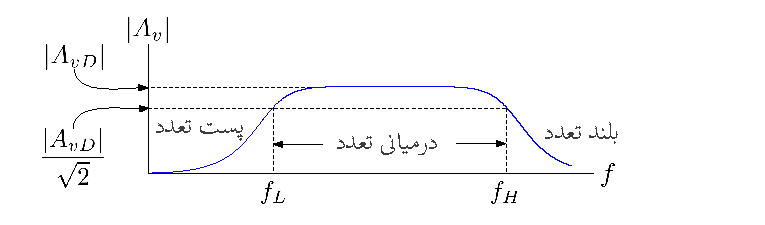
\includegraphics[scale=0.90]{freqResponse}
\caption{عمومی تعددی رد عمل}
\label{شکل_عمومی_تعددی_ردعمل}
\end{figure}
%
\begin{align} \label{مساوات_تعددی_ردعمل_دائرہ_کارکردگی}
B=f_H - f_L
\end{align}
اگر \عددی{f_H  \gg f_L} ہو تب \عددی{B \approx f_H} لکھا جا سکتا ہے یعنی
\begin{align} \label{مساوات_تعددی_ردعمل_دائرہ_کارکردگی_الف}
B \approx f_H
\end{align}
مشترکہ ایمٹر ٹرانزسٹر ایمپلیفائر تک داخلی اشارے کی رسائی عموماً بذریعہ \اصطلاح{جفتی کپیسٹر}\فرہنگ{کپیسٹر!جفتی}\فرہنگ{coupling capacitor} \عددیء{C_B}\حاشیہب{coupling capacitor} کی جاتی ہے جبکہ اس سے خارجی اشارے کی حصولی عموماً بذریعہ جفتی کپیسٹر \عددی{C_C}  کی جاتی ہے۔مزید یہ کہ \اصطلاح{قصری کپیسٹر}\فرہنگ{کپیسٹر!قصری}\حاشیہب{bypass capacitor}\فرہنگ{bypass capacitor}  \عددی{C_E} اشارے کو مزاحمت \عددی{R_E} کے متبادل راستہ فراہم کرتے ہوئے افزائش بڑھاتا ہے۔اس باب کے پہلے چند حصوں میں ان کپیسٹروں کا \اصطلاح{پست انقطاعی تعدد} کے ساتھ تعلق پر غور کیا جائے گا۔کم تعدد پر ان کپیسٹروں کی برقی رکاوٹ بڑھ جاتی ہے جس کی وجہ سے \عددی{A_v} ( \عددی{A_i} )  کی قیمت گھٹتی ہے۔یوں یہی بیرونی\حاشیہد{\عددیء{C_B}، \عددیء{C_E}، \عددی{C_C} وغیرہ بیرونی کپیسٹر ہیں جنہیں ٹرانزسٹر کے ساتھ جوڑا جاتا ہے} کپیسٹر پست انقطاعی تعدد \عددی{f_L} کی قیمت  تعین کرتے ہیں۔حقیقت میں پست انقطاعی تعدد \عددی{f_L} کا دارومدار کپیسٹر \عددی{C_E} پر ہوتا ہے۔بلند تعدد پر ان تمام بیرونی کپیسٹروں کی برقی رکاوٹ نہایت کم ہو جاتی ہے اور انہیں قصر دور تصور کیا جاتا ہے۔مثال \حوالہ{مثال_تعددی_رد_عمل_بیرونی_کپیسٹر_بلند_انقطاعی_نقطہ} میں بیرونی نسب کپیسٹر کی وجہ سے پیدا \اصطلاح{بلند انقطاعی نکتہ} دکھایا گیا ہے۔

ٹرانزسٹر کے \عددی{B-E}  اور \عددی{B-C} جوڑ پر اندرونی کپیسٹر \عددی{C_{b'e}} اور \عددی{C_{b'c}} پائے جاتے ہیں۔درمیانی تعدد اور اس سے کم تعدد پر ان اندرونی کپیسٹروں کی برقی رکاوٹ اتنی زیادہ ہوتی ہے کہ انہیں کھلے دور تصور کیا جاتا ہے۔بلند تعدد پر ان کی برقی رکاوٹ کم ہو جاتی ہے اور انہیں نظرانداز کرنا ممکن نہیں رہتا۔انہیں اندرونی کپیسٹروں کی وجہ سے بلند تعدد پر \عددی{A_v} ( \عددی{A_i})  کی قیمت گھٹتی ہے۔یوں اندرونی کپیسٹر بلند انقطاعی تعدد \عددی{f_H} کی قیمت تعین کرتے ہیں۔

کم تعدد پر ٹرانزسٹر ایمپلیفائر کی افزائش حاصل کرتے وقت صرف بیرونی کپیسٹروں کو مدِ نظر رکھا جاتا ہے جبکہ اندرونی کپیسٹروں کو کھلے دور تصور کیا جاتا ہے۔اسی طرح بلند تعدد پر صرف اندرونی کپیسٹروں کو مدِ نظر رکھا جاتا ہے جبکہ بیرونی کپیسٹروں کو قصر دور تصور کیا جاتا ہے اور درمیانی تعدد پر بیرونی کپیسٹروں کو قصر دور جبکہ اندرونی کپیسٹروں\حاشیہد{ٹرانزسٹر ریاضی نمونے میں پائے جانے والے کپیسٹر مثلاً \عددی{C{b'e}} وغیرہ ٹرانزسٹر کے اندرونی کپیسٹر ہیں} کو کھلے دور تصور کیا جاتا ہے۔

اس باب میں تمام مساوات \اصطلاح{لاپلاس بدل}\فرہنگ{لاپلاس بدل}\حاشیہب{Laplace transform}\فرہنگ{Laplace transform}  استعمال کرتے ہوئے \عددی{s} کے ساتھ لکھے جائیں گے۔سائن نما اشارات کے لئے \عددی{s}  کی جگہ \عددی{j \omega} لکھتے ہوئے جوابات حاصل کئے جاتے ہیں۔
	
\حصہ{بیس  سرے پر کپیسٹر \عددی{C_B}}ایمپلیفائر استعمال کرتے وقت اس کے داخلی اور خارجی جانب مختلف چیزیں جوڑی جا سکتی ہیں مثلاً لاوڈ سپیکر یا دوسرا ایمپلیفائر۔ایسی بیرونی اشیاء جوڑتے وقت یہ ضروری ہے کہ ٹرانزسٹر کا نقطہ کارکردگی اپنی جگہ برقرار رہے۔کپیسٹر یک سمتی برقی رو کے لئے کھلے سرے کردار ادا کرتا ہے لہٰذا کپیسٹر کے ذریعہ ایمپلیفائر کو داخلی جانب اشارہ فراہم کرنے یا ایمپلیفائر کے خارجی جانب سے کپیسٹر کے ذریعہ اشارہ حاصل کرنے سے ٹرانزسٹر کے نقطہ کارکردگی پر کوئی اثر نہیں ہوتا۔
\begin{figure}
\centering
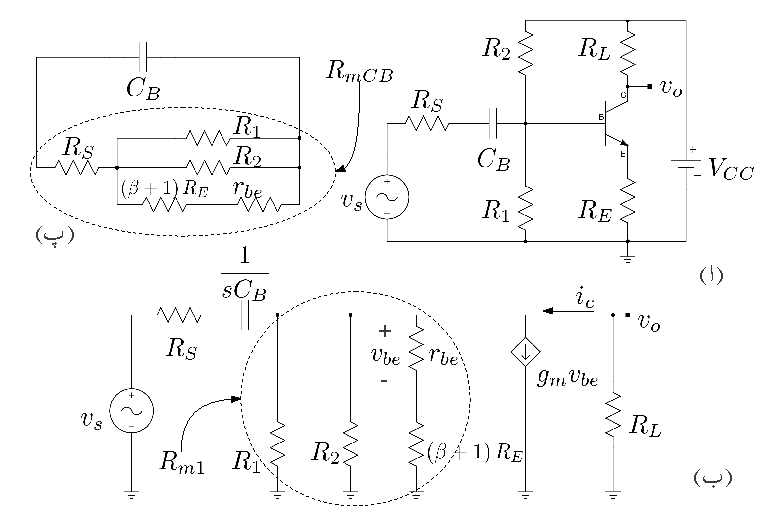
\includegraphics[scale=0.90]{amplifierWithCB}
\caption{کپیسٹر \عددی{C_B} کا کردار}
\label{شکل_قابو_کپیسٹر_کا_کردار}
\end{figure}
شکل \حوالہ{شکل_قابو_کپیسٹر_کا_کردار} الف میں ایسا ہی کرتے ہوئے کپیسٹر \عددی{C_B} کے ذریعہ داخلی اشارے کو ایمپلیفائر تک پہنچایا گیا ہے۔\عددی{C_B} پر توجہ رکھنے کی خاطر شکل میں \عددی{C_E} اور \عددی{C_C} نہیں استعمال کئے گئے۔شکل \حوالہ{شکل_قابو_کپیسٹر_کا_کردار} ب میں اسی کا مساوی باریک اشاراتی دور دکھایا گیا ہے جہاں نقطہ دار دائرے میں بند کل مزاحمت کو \عددی{R_{m1}} لکھا گیا ہے یعنی
\begin{align*}
\frac{1}{R_{m1}}=\frac{1}{R_1}+\frac{1}{R_2}+\frac{1}{r_{be}+\left(\beta+1 \right)R_E}
\end{align*}
شکل  ب کے لئے لکھا جا سکتا ہے۔
\begin{align*}
A_v&=\left( \frac{v_o}{i_c}\right ) \left( \frac{i_c}{v_{be}}\right ) \left( \frac{v_{be}}{v_b}\right ) \left( \frac{v_b}{v_s}\right )\\
&=\left(-R_L \right ) \left( g_m \right ) \left(\frac{r_{be}}{r_{be}+(\beta+1)R_E} \right ) \left(\frac{R_{m1}}{R_S+\frac{1}{s C_B}+R_{m1}} \right )\\
&=\left(-R_L \right ) \left(g_m \right ) \left(\frac{r_{be}}{r_{be}+(\beta+1)R_E} \right ) \left(\frac{s R_{m1} C_B}{s \left(R_S+R_{m1} \right ) C_B+1} \right )
\end{align*}
مندرجہ بالا مساوات میں \عددی{j \omega} کو \عددی{s} لکھا گیا ہے۔مساوات کے آخری قوسین میں کسر کے اوپر والے حصے سے \عددی{R_{m1}C_B}   اور اس کے نچلے حصے سے \عددی{\left( R_S+R_{m1}\right ) C_B}  باہر نکالتے ہوئے مندرجہ ذیل مساوات حاصل ہوتا ہے۔
\begin{align*}
A_v = -R_L  g_m  \left(\frac{r_{be}}{r_{be}+(\beta+1)R_E} \right ) \left (\frac{R_{m1}}{R_S+R_{m1}} \right ) \left(\frac{s}{s+\frac{1}{\left(R_S+R_{m1} \right )C_B}} \right )
\end{align*}
جیسے شکل \حوالہ{شکل_قابو_کپیسٹر_کا_کردار} پ میں وضاحت کی گئی ہے کہ \عددی{v_s} کو قصر دور تصور کرتے ہوئے، \عددی{C_B} کے متوازی کل مزاحمت کی قیمت \عددی{(R_S+R_{m1})} ہے جسے \عددی{R_{mCB}}\حاشیہد{\عددی{R_{mCB}} لکھتے ہوئے اس میں \عددی{R_m} سے مراد \اصطلاح{متوازی مزاحمت} جبکہ \عددی{CB} سے مراد کپیسٹر \عددی{C_B} ہے}  لکھتے ہوئے اس مساوات کو یوں لکھا جا سکتا ہے۔
\begin{align} \label{مساوات_تعددی_ردعمل_ایمپلیفائر_بمع_قابو_کپیسٹر}
A_v=-R_L  g_m \left(\frac{r_{be}}{r_{be}+(\beta+1)R_E} \right ) \left (\frac{R_{m1}}{R_S+R_{m1}} \right ) \left(\frac{s}{s+\frac{1}{R_{mCB} C_B}} \right )
\end{align}
اگر اس مساوات میں تعدد \عددی{\omega} کی قیمت بتدریج بڑھائی جائے تو آخری قوسین کی قیمت ایک \عددی{(1)}  تک پہنچنے کی کوشش کرے گی۔ اگرچہ اس مساوات کو حاصل کرنے کی خاطر ٹرانزسٹر کا پست تعدد ریاضی نمونہ استعمال کیا گیا تھا جو صرف کم  اور درمیانی تعدد کے لئے درست ہے مگر فی الحال اس بحث میں پڑے بغیر تصور کرتے ہیں کہ \عددی{\omega} کی قیمت لامحدود کر دی جاتی ہے۔یوں
\begin{align*}
\eval{A_v}_{\omega \to \infty} \hspace{-2em}=-R_L g_m  \left(\frac{r_{be}}{r_{be}+(\beta+1)R_E} \right ) \left (\frac{R_{m1}}{R_S+R_{m1}} \right ) \left(\frac{\infty}{\infty+\frac{1}{R_{mCB} C_B}} \right )
\end{align*}
حاصل ہوتا ہے جسے \اصطلاح{درمیانی تعدد کی افزائش} \عددی{A_{vD}} کہتے ہیں۔
\begin{align} \label{مساوات_تعددی_ردعمل_قابو_کپیسٹر_لامحدود_تعدد}
A_{vD}=\eval{A_v}_{\omega \to \infty}=-R_L g_m  \left(\frac{r_{be}}{r_{be}+(\beta+1)R_E} \right ) \left (\frac{R_{m1}}{R_S+R_{m1}} \right ) 
\end{align}
\عددی{A_{vD}} کو نلکی محدد  کے طرز پر یوں لکھا جا سکتا ہے۔
\begin{align}
A_{vD} = \left | {A_{vD}}  \right | \phase{ \theta_D}
\end{align}
جہاں
\begin{align}
\left | A_{vD} \right | &= \left (R_L \right ) \left (g_m \right ) \left (\frac{r_{be}}{r_{be}+\left(\beta+1 \right ) R_E} \right ) \left (\frac{R_{m1}}{R_S+R_{m1}} \right )\\
\theta_D &=\pi
\end{align}
کے برابر ہیں۔مندرجہ بالا مساوات میں \عددی{\abs{A_{vD}}}  افزائش کی حتمی قیمت جبکہ \عددی{\theta_D}  افزائش کا زاویہ ہے۔ \عددی{A_{vD}}  کے استعمال سے مساوات \حوالہ{مساوات_تعددی_ردعمل_ایمپلیفائر_بمع_قابو_کپیسٹر}  کو مندرجہ ذیل طریقے سے لکھ سکتے ہیں۔
\begin{gather} \label{مساوات_تعددی_ردعمل_قابو_کپیسٹر_لامحدود_کا_استعمال}
\begin{aligned}
A_v&=A_{vD} \left(\frac{s}{s+\frac{1}{R_{mCB} C_B}} \right )
\end{aligned}
\end{gather}
مساوات \حوالہ{مساوات_تعددی_ردعمل_ایمپلیفائر_بمع_قابو_کپیسٹر} کو نلکی محدد کے طرز پر یوں لکھا جا سکتا ہے
\begin{align}
A_v =\abs{A_{v}} \phase{\theta}
\end{align}
جہاں

\begin{gather} \label{مساوات_تعددی_ردعمل_قابو_کپیسٹر_حیطہ_اور_زاویہ}
\begin{aligned}
\abs{A_v} &=\abs{A_{vD}} \frac{\omega}{\sqrt{\omega^2 +\left(\frac{1}{R_{mCB} C_B} \right )^2}}\\
\theta&=-\frac{\pi}{2}-\tan^{-1}\left(\omega R_{mCB} C_B \right )
\end{aligned}
\end{gather}
ہیں۔اگرچہ مساوات \حوالہ{مساوات_تعددی_ردعمل_قابو_کپیسٹر_لامحدود_تعدد} حتمی طور پر صرف لامحدود تعدد کے لئے درست ہے لیکن جیسے آپ مثال \حوالہ{مثال_تعددی_ردعمل_مختلف_تعدد_پر_افزائش}  میں دیکھیں گے کہ درمیانی سطح کے تعدد کے لئے بھی یہی مساوات صحیح جوابات دیتا ہے۔یوں \عددی{A_{vD}}  کو ایمپلیفائر کی \اصطلاح{درمیانی تعدد کی افزائش} کہتے ہیں۔

%==========
\ابتدا{مثال} \شناخت{مثال_تعددی_ردعمل_مختلف_تعدد_پر_افزائش}
شکل  \حوالہ{شکل_قابو_کپیسٹر_کا_کردار} الف میں گزشتہ کئی مثالوں کی طرح
\begin{align*} 
V_{\textup{CC}}&=\SI{15}{\volt} & \beta &=\num{179}\\ 
R_{\textup {L}}&=\SI{75}{\kilo \ohm} & R_{\textup {E}}&=\SI{15}{\kilo \ohm}\\
R_{\textup {1}}&=\SI{320}{\kilo \ohm} & R_{\textup {2}}&=\SI{1.7}{\mega \ohm}\\
R_{\textup {s}}&=\SI{5}{\kilo \ohm} & C_{\textup{B}}&=\SI{0.1}{\nano \farad}
\end{align*}
  لیتے ہوئے مندرجہ ذیل تعدد پر افزائش \عددی{A_v}  حاصل کریں۔
\begin{enumerate}
\item
لا محدود
\item
$
\begin{aligned}[t]
f=\SI{1}{\mega \hertz}
\end{aligned}
$
\item
$
\begin{aligned}[t]
f=\SI{100}{\kilo \hertz}
\end{aligned}
$
\item
$
\begin{aligned}[t]
f=\SI{10}{\kilo \hertz}
\end{aligned}
$
\item
$
\begin{aligned}[t]
f=\SI{1}{\kilo \hertz}
\end{aligned}
$
\end{enumerate}

حل: یک سمتی  تجزیہ سے مندرجہ ذیل \عددی{g_m}، \عددی{r_{b'e}} اور \عددی{r_e} حاصل ہوتے ہیں۔
\begin{align*}
g_m&=\SI{4.064}{\milli \siemens}\\
r_{be}&=\SI{44.045}{\kilo \ohm}\\
r_e& \approx \SI{246}{\ohm}
\end{align*}
%
\begin{enumerate}
\item
لامحدود تعدد یعنی \عددی{f=\infty}  پر مساوات \حوالہ{مساوات_تعددی_ردعمل_قابو_کپیسٹر_لامحدود_تعدد}  کی مدد سے \عددی{A_{vD}} کی قیمت

\begin{align*}
A_{vD}&=\left ( -75000 \right ) \left( 0.004064 \right) \left (\frac{44045}{44045+180 \times 15000} \right ) \left (\frac{245238}{5000+245238} \right ) \\ 
&=-4.79463\\
&=4.79463 \phase {\pi}
\end{align*}
حاصل ہوتا ہے جہاں آخری قدم پر افزائش کو نلکی محدد  کے طرز پر لکھا گیا ہے۔اس جواب کے مطابق داخلی اشارے کا حیطہ \عددی{\num{4.79463}} گنا بڑھے گا اور اس کے زاویہ میں  \عددی{\pi} ریڈیئن یعنی \عددی{\SI{180}{\degree}} کی تبدیلی رونما ہو گی۔
\item
\عددی{1 MHz} پر مساوات \حوالہ{مساوات_تعددی_ردعمل_قابو_کپیسٹر_لامحدود_کا_استعمال}  کی مدد سے
\begin{align*}
A_v &=\frac{-4.79463}{1 + \frac{1}{j \times 2 \times \pi \times 10^{6} \times  (5000+245238) \times 0.1 \times 10^{-9}}} \\
&=-4.79443-j 0.03049\\
&=4.7945 \phase {-3.13523}
\end{align*}
حاصل ہوتا ہے۔آپ دیکھ سکتے ہیں کہ افزائش کی حتمی قیمت لامحدود تعدد پر\عددی{\num{4.79463}} تھی جبکہ اب اس کی قیمت \عددی{\num{4.7945}} ہو گئی ہے۔ان دو قیمتوں میں فرق کو نظر انداز کیا جا سکتا ہے۔زاویہ \عددی{\SI{-179.635}{\degree}} یعنی یعنی تقریباً \عددی{\SI{180.36}{\degree}} ہے۔
\item
\عددی{f=\SI{100}{\kilo \hertz}}	پر
\begin{align*}
A_v &=\frac{-4.79463}{1 + \frac{1}{j \times 2 \times \pi \times 100 \times 10^{3} \times  (5000+245238) \times 0.1 \times 10^{-9}}} \\
&=-4.7753-j 0.30372\\
&=4.78495 \phase {-3.0781}
\end{align*}
حاصل ہوتا ہے۔اب بھی افزائش تقریباً \عددی{A_{vD}} کے برابر ہے۔
\item
\عددی{f=\SI{10}{\kilo \hertz}} پر
\begin{align*}
A_v &=\frac{-4.79463}{1 + \frac{1}{j \times 2 \times \pi \times 10 \times 10^{3} \times  (5000+245238) \times 0.1 \times 10^{-9}}} \\
&=-3.4137-j 2.1712\\
&=4.04567 \phase {-2.5751}
\end{align*}
حاصل ہوتا ہے۔ہم دیکھتے ہیں کہ \عددی{\SI{10}{\kilo \hertz}}  پر افزائش کی قیمت قدرِ کم ہو گئی ہے یعنی اس کی موجودہ قیمت \عددی{A_{vD}}  کے  \عددی{\SI{84}{\percent}} ہے 
\begin{align*}
\frac{4.04567}{4.79463} \times 100=\SI{84}{\percent}
\end{align*}
جبکہ زاویہ \عددی{\SI{-147}{\degree}} ہے۔
%
\item
\عددی{f=\SI{1}{\kilo \hertz}}  پر
\begin{align*}
A_v &=\frac{-4.79463}{1 + \frac{1}{j \times 2 \times \pi \times 1 \times 10^{3} \times  (5000+245238) \times 0.1 \times 10^{-9}}} \\
&=-0.1157-j 0.7357\\
&=0.7447 \phase {-1.7268}
\end{align*}
حاصل ہوتا ہے جو کہ نہایت کم افزائش ہے۔ایک کلو ہرٹز کے تعدد پر حاصل کی گئی افزائش \عددی{A_{vD}} کے صرف \عددی{\SI{15}{\percent}}  ہے۔
\begin{align*}
\frac{0.7447}{4.79463} \times 100=\SI{15}{\percent}
\end{align*}
ایک کلو ہرٹز کے کم تعدد پر افزائش کا نہایت کم ہوجانا صاف ظاہر ہے۔
\end{enumerate}
\انتہا{مثال}
%===========
مندرجہ بالا مثال میں ہم نے دیکھا کہ ایک خاص حد سے زیادہ تعدد پر افزائش کی قیمت کو تقریباً \عددی{A_{vD}} کے برابر تصور کیا جا سکتا ہے۔البتہ اس حد سے کم تعدد پر افزائش کی قیمت کم ہو جاتی ہے۔\اصطلاح{بوڈا خط}\فرہنگ{بوڈا خط}\حاشیہب{Bode plot}\فرہنگ{Bode plot} اس قسم کے معلومات کو ظاہر کرنے کا ایک نہایت عمدہ طریقہ ہے۔موجودہ مسئلے میں افزائش بالمقابل تعدد کو \اصطلاح{بوڈا خط} کے طرز پر شکل \حوالہ{شکل_پست_انقطاعی_تعدد_الف} میں کھینچا گیا ہے جہاں تعدد کو \اصطلاح{لوگارتھم}\حاشیہب{log}  پیمانے پر دکھایا گیا ہے۔اس شکل میں زیادہ تعدد پر افزائش تبدیل نہیں ہوتی اور \عددی{\abs{A_{vD}}}  ہی رہتی ہے۔حقیقت میں \اصطلاح{بلند تعدد}\فرہنگ{بلند تعدد}\حاشیہب{high frequency} پر بھی افزائش کم پڑ جاتی ہے۔موجودہ حصے میں صرف \اصطلاح{پست تعدد}\فرہنگ{پست تعدد}\حاشیہب{low frequency} پر افزائش کے کم ہونے پر غور کیا جائے گا۔زیادہ تعدد پر افزائش کے کم ہونے پر آگے جا کر غور کیا جائے گا۔
\begin{figure}
\centering
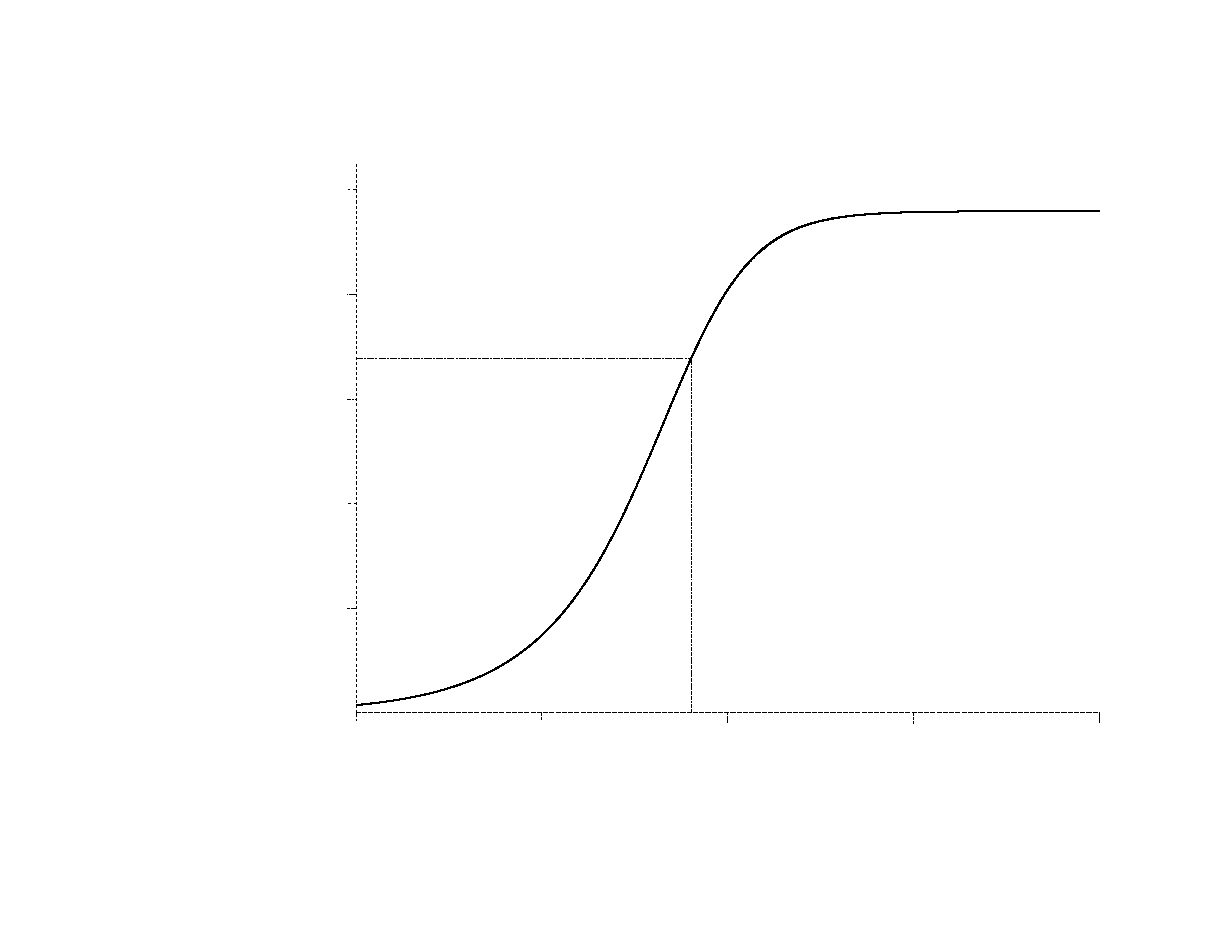
\includegraphics[scale=0.90]{lowCutoffFrequencyA}
\caption{ پست انقطاعی تعدد}
\label{شکل_پست_انقطاعی_تعدد_الف}
\end{figure}
شکل کو دیکھتے ہوئےہم کہہ سکتے ہیں کہ کم تعدد پر یہ ایمپلیفائر داخلی اشارہ کو نہیں بڑھائے گا۔تعدد بتدریج کم کرتے ہوئے، جس تعدد پر افزائش کی قیمت کم ہوتے ہوتے \عددی{\abs{A_{vD}}} کے \عددی{\frac{1}{\sqrt{2}}} گنا ہو جائے اسی کو انقطاعی نقطہ  تصور کیا جاتا ہے۔شکل  \حوالہ{شکل_پست_انقطاعی_تعدد_الف} میں \عددی{f=\SI{6360}{\hertz}} پر \عددی{\abs{A_v}=\frac{\abs{A_{vD}}}{\sqrt{2}}} ہو جاتا ہے۔یوں ہم کہیں گے کہ یہ ایمپلیفائر  \عددی{\SI{6360}{\hertz}} سے کم تعدد کے اشارات کو نہیں بڑھاتا۔جیسا کہ پہلے ذکر کیا گیا، زیادہ تعدد پر بھی ایمپلیفائر کی افزائش کم ہوجاتی ہے یوں موجودہ نقطے کا پورا نام \اصطلاح{پست انقطاعی نکتہ} ہے جبکہ اس نقطے پر تعدد \عددی{f_L} کو \اصطلاح{پست انقطاعی تعدد}\فرہنگ{پست انقطاعی تعدد}\حاشیہب{low cut-off frequency}  پکارا جاتا ہے۔


مساوات \حوالہ{مساوات_تعددی_ردعمل_قابو_کپیسٹر_حیطہ_اور_زاویہ} سے ہم پست انقطاعی تعدد حاصل کر سکتے ہیں۔ایسا کرنے کی خاطر اس تعدد کو \عددی{\omega_L} لکھتے ہوئے مساوات کو \عددی{\abs{A_v}=\frac{\abs{A_{vD}}}{\sqrt{2}}} (یعنی درمیانی تعدد پر افزائش سے \عددی{\SI{3}{dB}}  کم ) کے لئے حل کرتے ہیں
\begin{align*}
\frac{\abs{A_{vD}}}{\sqrt{2}} &=\abs{A_{vD}} \frac{\omega_L}{\sqrt{\omega_L^2 +\left(\frac{1}{R_{mCB} C_B} \right )^2}}\\
\frac{1}{\sqrt{2}}&= \frac{\omega_L}{\sqrt{\omega_L^2 +\left(\frac{1}{R_{mCB} C_B} \right )^2}}
\end{align*}
دونوں جانب کا مربع لیتے ہوئے
\begin{align*}
\frac{1}{2}&= \frac{\omega_L^2}{\omega_L^2 +\left(\frac{1}{R_{mCB} C_B} \right )^2}
\end{align*}
سے
\begin{gather} \label{مساوات_تعددی_ردعمل_قابو_کپیسٹر_پست_انقطاعی_تعدد}
\begin{aligned}
\omega_L &= \frac{1}{R_{mCB} C_B}\\
f_L&=\frac{1}{2 \pi  R_{mCB} C_B}
\end{aligned}
\end{gather}
ہو۔ اس طرح مساوات \حوالہ{مساوات_تعددی_ردعمل_قابو_کپیسٹر_لامحدود_کا_استعمال}  لکھنے کا بہتر انداز یوں ہے ۔
\begin{align} \label{مساوات_تعددی_ردعمل_قابو_کپیسٹر_معیاری_مساوات}
A_v=A_{vD} \left(\frac{s}{s+\omega_L} \right )
\end{align}
مندرجہ بالا مساوات اور شکل \حوالہ{شکل_قابو_کپیسٹر_کا_کردار}  کو ایک ساتھ دیکھتے ہوئے معلوم ہوتا ہے کہ \عددی{f_L}  کی قیمت داخلی کپیسٹر \عددی{C_B}  اور اس کے ساتھ متوازی کل مزاحمت \عددی{R_{mCB}}  پر منحصر ہے۔مثال \حوالہ{مثال_تعددی_ردعمل_مختلف_تعدد_پر_افزائش}  میں یوں
\begin{align*}
f_L=\frac{1}{2 \pi \left(5000+245238 \right ) \times 0.1 \times 10^{-9}  }=\SI{6360}{\hertz}
\end{align*}
حاصل ہوتا ہے۔
%=========
\ابتدا{مثال}
مندرجہ بالا مثال \حوالہ{مثال_تعددی_ردعمل_مختلف_تعدد_پر_افزائش} میں صرف\عددی{C_B} کی قیمت تبدیل کرتے ہوئے ایمپلیفائر کو انسانی آواز کا حیطہ بڑھانے کے قابل بنائیں۔

حل: انسان \عددی{\SI{20}{\hertz}} تا \عددی{\SI{20}{\kilo \hertz}} کی آواز سن سکتا ہے۔اگر \عددی{C_B} کو  \عددی{\SI{20}{\hertz}} گزارنے کی غرض سے منتخب کیا جائے تو یہ اس سے زیادہ تمام تعدد کے اشارات کو بھی گزارے گا اور یوں \عددی{\SI{20}{\kilo \hertz}} کے اشارے کو کوئی مسئلہ درپیش نہیں آئے گا۔اگرچہ \عددی{f_L}  کو \عددی{\SI{20}{\hertz}}  پر رکھتے ہوئے بھی \عددی{C_B} حاصل کیا جاتا ہے لیکن ہم جانتے ہیں کہ \عددی{f_L} پر افزائش کم ہو جاتی ہے لہٰذا ہم \عددی{f_L}  کو درکار تعدد سے دس گنا کم یعنی \عددی{\SI{2}{\hertz}}  پر رکھتے ہوئے مساوات \حوالہ{مساوات_تعددی_ردعمل_قابو_کپیسٹر_پست_انقطاعی_تعدد}  کی مدد سے \عددی{C_B} حاصل کرتے ہیں۔
\begin{align*}
C_B&=\frac{1}{2 \pi f_L \left(R_{mCB} \right ) }\\
&=\frac{1}{2 \pi \times 2 \times 250238 }\\
&=0.318 \times 10^{-6}= \SI{0.318}{\micro \farad}
\end{align*}
\انتہا{مثال}
%=========
\حصہ{ایمٹر سرے پر کپیسٹر \عددی{C_E}}
ٹرانزسٹر کا نقطہ کارکردگی تعین کرنے کے علاوہ \عددی{\beta}  میں تبدیلی سے  نقطہ کارکردگی میں تبدیلی رونما ہونے کو \عددی{R_E} کے استعمال سے کم کیا جاتا ہے۔البتہ ایمپلیفائر کی افزائش بڑھانے کے  لئے یہ ضروری ہے کہ ٹرانزسٹر کے ایمٹر سرے پر کم سے کم مزاحمت ہو۔ان دو متضاد شرائط پر پورا اترتا دور شکل \حوالہ{شکل_مخارج_کپیسٹر_کا_کردار} الف میں دکھایا گیا ہے۔چونکہ کپیسٹر \عددی{C_E} یک سمتی برقی رو کے لئے کھلے دور کا کردار ادا کرتا ہے لہٰذا اس کے استعمال سے یک سمتی متغیرات متاثر نہیں ہوتے۔\عددی{C_E} کو یوں چنا جاتا ہے کہ درکار تعدد پر اس کی \اصطلاح{برقی رکاوٹ}\فرہنگ{برقی!رکاوٹ}\حاشیہب{impedance} \عددی{R_E} سے کم ہو۔چونکہ \عددی{C_E} مزاحمت \عددی{R_E} کے متوازی جڑا ہے لہٰذا بدلتی رو کے نقطہ نظر سے ٹرانزسٹر کے ایمٹر پر کل رکاوٹ \عددی{R_E} سے کم ہو جاتی ہے اور یوں افزائش بڑھتی ہے۔اس حصے میں \عددی{C_E} پر توجہ رکھنے کی خاطر \عددی{C_B} اور \عددی{C_C} کا استعمال نہیں کیا گیا۔

شکل \حوالہ{شکل_مخارج_کپیسٹر_کا_کردار} ب میں شکل \حوالہ{شکل_مخارج_کپیسٹر_کا_کردار} الف کا مساوی باریک اشاراتی دور دکھایا گیا ہے جس سے ہم افزائش کی مساوات لکھ سکتے ہیں۔باریک اشاراتی دور میں بیس  جانب کے مزاحمت کے عکس ایمٹر جانب دکھائے گئے ہیں۔جیسا کہ آپ جانتے ہیں کہ ایمٹر جانب کے مزاحمت کا عکس،  بیس  جانب \عددی{(\beta+1)} گنا زیادہ نظر آتا ہے جبکہ بیس  جانب مزاحمت کا عکس، ایمٹر جانب \عددی{(\beta+1)} گنا کم نظر آتا ہے۔یوں بیس  جانب کے مزاحمت \عددی{R_B} اور \عددی{r_{be}} کے عکس، ایمٹر جانب \عددی{\frac{R_B}{\beta+1}} اور \عددی{\frac{r_{be}}{\beta+1}} نظر آئیں گے۔
\begin{gather} \label{مساوات_تعددی_ردعمل_مخارج_کپیسٹر_کا_کردار}
\begin{aligned} 
A_v&=\left(\frac{v_o}{i_c} \right ) \left(\frac{i_c}{v_{be}} \right ) \left(\frac{v_{be}}{v_s} \right )\\
&=\left(-R_L \right ) \left(g_m \right ) \left (\frac{r_e}{\frac{R_B}{\beta+1}+r_e+Z_E }\right )
\end{aligned}
\end{gather}
جہاں
\begin{gather} \label{مساوات_تعددی_ردعمل_مخارج_کپیسٹر_اور_رکاوٹ}
\begin{aligned}
\frac{1}{Z_E}&=s C_E+\frac{1}{R_E}\\
Z_E&=\frac{1}{s C_E +\frac{1}{R_E}}
\end{aligned}
\end{gather}
%
\begin{figure}
\centering
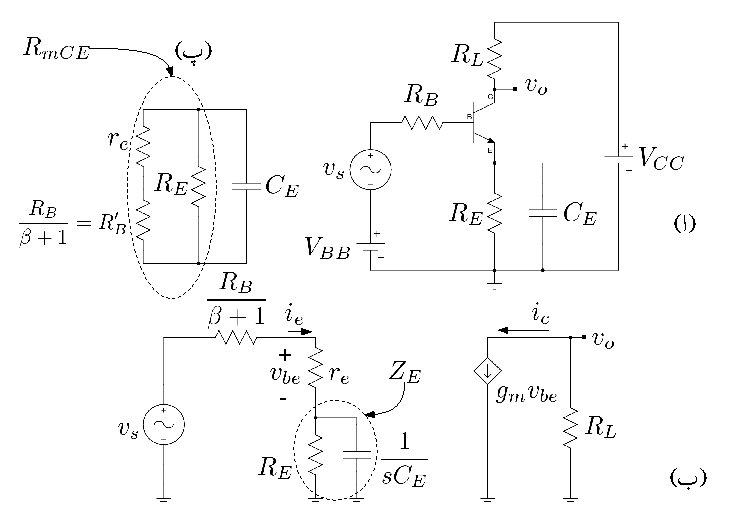
\includegraphics[scale=0.90]{amplifierWithCE}
\caption{کپیسٹر \عددی{C_E} کا کردار}
\label{شکل_مخارج_کپیسٹر_کا_کردار}
\end{figure}
اور
\begin{align}
r_e=\frac{r_{be}}{\beta+1}
\end{align}
ہیں۔شکل  ب میں \عددی{v_s}  کو نظر انداز کرتے ہوئے  \عددی{C_E} کے متوازی کل مزاحمت کو \عددی{R_{mCE}} لکھتے ہوئے ہم دیکھتے ہیں کہ
\begin{align} \label{مساوات_تعددی_ردعمل_مخارج_کپیسٹر_کے_متوازی_مزاحمت}
\frac{1}{R_{mCE}}=\frac{1}{R_E}+\frac{1}{\frac{R_B}{\beta+1}+r_e}=\frac{1}{R_E}+\frac{1}{R_B'+r_e}
\end{align}
کے برابر ہے۔شکل  پ میں اس مزاحمت کی وضاحت کی گئی ہے۔

مساوات \حوالہ{مساوات_تعددی_ردعمل_مخارج_کپیسٹر_کا_کردار}  میں \عددی{\frac{R_B}{\beta+1}} کو \عددی{R_B'} لکھتے ہوئے اور اس میں مساوات \حوالہ{مساوات_تعددی_ردعمل_مخارج_کپیسٹر_اور_رکاوٹ}  سے \عددی{Z_E}  کی قیمت استعمال کرتے ہوئے حل کرتے ہیں۔
\begin{align*}
A_v&=\left(-R_L \right ) \left(g_m \right ) \left(\frac{r_e}{R_B'+r_e+\frac{1}{s C_E+\frac{1}{R_E}}} \right )
\end{align*}
آخری قوسین کو \عددی{\left(s C_E +\tfrac{1}{R_E} \right)} سے ضرب اور تقسیم کرتے ہیں۔
\begin{align*}
A_v&=-R_L g_m r_e \left(\frac{s C_E+\frac{1}{R_E}}{\left(R_B'+r_e \right ) \left(s C_E+\frac{1}{R_E} \right )+1 } \right )\\
&=-R_L g_m r_e \left (\frac{sC_E+\frac{1}{R_E}}{sC_E(R_B'+r_e) +\frac{(R_B'+r_e)}{R_E}+1} \right )
\end{align*}
نچلے  جانب \عددی{\left (R_B'+r_e \right)} باہر نکالتے ہیں۔
\begin{align*}
A_v&=-\frac{R_L g_m r_e}{(R_B'+r_e)} \left(\frac{sC_E+\frac{1}{R_E}}{sC_E+\frac{1}{R_E} +\frac{1}{R_B'+r_e}} \right )
\end{align*}
اس مساوات کے آخری قدم پر مساوات \حوالہ{مساوات_تعددی_ردعمل_مخارج_کپیسٹر_کے_متوازی_مزاحمت}  استعمال کرتے ہوئے اسے مزید حل کرتے ہیں۔
\begin{align*}
A_v=-\left( \frac{R_L g_m r_e}{R_B'+r_e} \right ) \left(\frac{sC_E+\frac{1}{R_E}}{sC_E+\frac{1}{R_{mCE}}} \right )
\end{align*}
کسر کے اوپر اور نیچے سے \عددی{C_E} باہر نکالتے ہوئے حاصل ہوتا ہے۔
\begin{align}
A_v=-\left( \frac{R_L g_m r_e}{R_B'+r_e} \right ) \left(\frac{s+\frac{1}{R_E C_E}}{s+\frac{1}{R_{mCE} C_E}} \right )
\end{align}
اس کو مساوات \حوالہ{مساوات_تعددی_ردعمل_قابو_کپیسٹر_معیاری_مساوات} کے طرز پر لکھتے ہیں یعنی
\begin{align} \label{مساوات_تعددی_ردعمل_مخارج_کپیسٹر_معیاری_مساوات}
A_v&=A_{vD} \left(\frac{s+\omega_1}{s+\omega_2} \right )
\end{align}
یا
\begin{gather}
\begin{aligned} \label{مساوات_تعددی_ردعمل_مخارج_کپیسٹر_معیاری_مساوات_الف}
A_v&=A_{vD} \left(\frac{j \omega+\omega_1}{j \omega+\omega_2} \right )\\
&=A_{vD} \left(\frac{j 2 \pi f+2 \pi f_1}{j 2 \pi f+ 2 \pi f_2} \right )\\
&=A_{vD} \left(\frac{j  f+f_1}{j f+f_2} \right )\\
\end{aligned}
\end{gather}
جہاں
\begin{gather} \label{مساوات_تعددی_ردعمل_مخارج_کپیسٹر_انقطاعی_تعدد}
\begin{aligned}
\omega_1&=2 \pi f_1=\frac{1}{R_E C_E}\\  
\omega_2&=2 \pi f_2=\frac{1}{R_{mCE}C_E}
\end{aligned}
\end{gather}
اور
\begin{align}\label{مساوات_تعددی_ردعمل_مخارج_کپیسٹر_درمیانی_تعدد_افزائش}
A_{vD}&=-\left(\frac{R_L g_m r_e}{R_B'+r_e}\right)
\end{align}
کے برابر ہیں۔کسی بھی تعدد  \عددی{\omega} پر
\begin{align}
\abs{A_v}=\abs{A_{vD}} \frac{\sqrt{\omega^2+\omega_1^2}}{\sqrt{\omega^2+\omega_2^2}}
\end{align}
ہو گا۔

مساوات \حوالہ{مساوات_تعددی_ردعمل_مخارج_کپیسٹر_معیاری_مساوات} میں \عددی{\omega} کی قیمت کو \عددی{\omega_1} اور \عددی{\omega_2} سے بہت زیادہ تصور کرتے ہوئے افزائش کی قیمت  حاصل کرتے ہیں۔  اس زیادہ تعدد کو  \عددی{\omega \to \infty}  تصور کرتے ہوئے
\begin{gather} \label{مساوات_تعددی_ردعمل_مخارج_کپیسٹر_لامحدود_تعدد}
\begin{aligned}
\eval{A_{v}}_{\omega \to \infty}&=A_{vD} \left(\frac{j \infty+\omega_1}{j \infty+\omega_2} \right ) =A_{vD}
\end{aligned}
\end{gather}
حاصل ہوتا ہے۔یوں \عددی{A_{vD}} درمیانی تعدد پر افزائش ہے۔

عموماً ایمپلیفائر مساوات \حوالہ{مساوات_ٹرانزسٹر_مخارج_قابو_مزاحمت_کی_شرح} کے تحت تخلیق دئے جاتے ہیں جس کے مطابق \عددی{R_E} کی قیمت \عددی{\frac{R_B}{(\beta+1)}} سے بہت زیادہ ہوتی ہے۔اگر مساوات \حوالہ{مساوات_ٹرانزسٹر_مخارج_قابو_مزاحمت_کی_شرح} کے شرط کو قدرِ تبدیل کر کے یوں بیان کیا جائے کہ
\begin{align} \label{مساوات_تعددی_ردعمل_مخارج_قابو_مزاحمت_کی_شرح}
R_E \gg \frac{R_B}{\beta+1}+r_e
\end{align}
تب مساوات \حوالہ{مساوات_تعددی_ردعمل_مخارج_کپیسٹر_معیاری_مساوات} کا \اصطلاح{صفر}\فرہنگ{صفر}\حاشیہب{zero}\فرہنگ{zero} اس کے \اصطلاح{قطب}\فرہنگ{قطب}\حاشیہب{pole}\فرہنگ{pole} سے کم تعدد پر پایا جائے گا یعنی
\begin{align} \label{مساوات_تعددی_ردعمل_بلند_تعدد_پست_سے_نہایت_زیادہ}
\omega_1 \ll \omega_2
\end{align}
عموماً \عددی{\tfrac{R_B}{\beta+1}\gg r_e} ہوتا ہے اور یوں مساوات \حوالہ{مساوات_تعددی_ردعمل_مخارج_قابو_مزاحمت_کی_شرح}  اور مساوات \حوالہ{مساوات_ٹرانزسٹر_مخارج_قابو_مزاحمت_کی_شرح} کو تقریباً ایک ہی شرط تصور کیا جا سکتا ہے۔افزائش \عددی{\abs{A_v}}  اس وقت درمیانی تعدد کے \عددی{\abs{A_{vD}}} سے \عددی{\SI{3}{\deci \bel}}  کم ہو گی جب
\begin{align}
\abs{A_v}=\abs{A_{vD}} \sqrt{\frac{\omega_L^2 + \omega_1^2}{\omega_L^2 +\omega_2^2}}=\frac{\abs{A_{vD}}}{\sqrt{2}}
\end{align}
ہو۔مندرجہ بالا مساوات میں مطلوبہ تعدد کو \عددی{\omega_L} لکھا گیا ہے جسے حل کرتے حاصل ہوتا ہے
\begin{align} \label{مساوات_تعددی_ردعمل_پست_انقطاعی_تعدد_سادہ_مساوات}
\omega_L=\sqrt{\omega_2^2 -2 \omega_1^2} \approx \omega_2
\end{align}
جہاں مساوات \حوالہ{مساوات_تعددی_ردعمل_بلند_تعدد_پست_سے_نہایت_زیادہ} کے تحت \عددی{\omega_1} کو نظر انداز کیا گیا ہے۔اگر \عددی{\omega_2^2} کی قیمت \عددی{2 \omega_1^2} سے کم ہو تب مندرجہ بالا مساوات کے تحت \عددی{\abs{A_v}} کبھی بھی \عددی{\abs{A_{vD}}}  سے \عددی{\SI{3}{\deci \bel}}  کم نہیں ہو گا اور یوں \عددی{\omega_L} نہیں پایا جائے گا۔

%============
\ابتدا{مثال}
شکل \حوالہ{شکل_مخارج_کپیسٹر_کا_کردار} الف میں
\begin{align*}
V_{\textup{CC}} &=\SI{15}{\volt} & V_{\textup{BB}} &=\SI{2.376}{\volt} \\
R_{\textup{L}} &=\SI{75}{\kilo \ohm} &  R_{\textup{E}} &=\SI{15}{\kilo \ohm}\\
R_{\textup{B}} &=\SI{269.3}{\kilo \ohm} & \beta &=\num{179}\\
C_{\textup{E}}&=\SI{10}{\nano \farad}
\end{align*}
ہیں۔ \عددی{A_{vD}} اور \عددی{f_L} حاصل کرتے ہوئے \عددی{\abs{A_v}} کا خط کھینچیں۔

حل: ان قیمتوں سے
\begin{align*}
I_C&=\frac{V_{BB}-V_{BE}}{\frac{R_B}{\beta+1}+R_E}=\frac{2.376-0.7}{\frac{269.3 \times 10^3}{179+1}+15000}=\SI{101.6}{\micro \ampere}\\
g_m&=\frac{I_C}{V_T}=\frac{101.6 \times 10^{-6}}{25 \times 10^{-3}}=\SI{4.064}{\milli \siemens}\\
r_e&=\frac{1}{4.064 \times 10^{-3}}=\SI{246}{\ohm}
\end{align*}
اور
\begin{align*}
\frac{1}{R_{mCE}}&=\frac{1}{15000}+\frac{1}{\frac{269300}{179+1}+246}\\
R_{mCE}&=\SI{1560.83}{\ohm}
\end{align*}
حاصل ہوتے ہیں۔یوں \عددی{\frac{R_B}{\beta+1}+r_e=\SI{1742}{\ohm}} بنتا ہے جو کہ \عددی{R_E} سے بہت کم ہے۔ مساوات \حوالہ{مساوات_تعددی_ردعمل_مخارج_کپیسٹر_انقطاعی_تعدد}  کے تحت
\begin{align*}
\omega_1&=\frac{1}{15000 \times 10 \times 10^{-9}}=\SI[per=frac,fraction=nice]{6666}{\radian \per \second}\\
\omega_2&=\frac{1}{1560.83 \times 10 \times 10^{-9}}=\SI[per=frac,fraction=nice]{64068}{\radian \per \second}
\end{align*}
حاصل ہوتے ہیں۔چونکہ \عددی{\omega_2^2}  کی قیمت \عددی{2 \omega_1^2} کے قیمت سے زیادہ ہے لہٰذا مساوات \حوالہ{مساوات_تعددی_ردعمل_پست_انقطاعی_تعدد_سادہ_مساوات}  کے تحت
\begin{align*}
\omega_L&=\sqrt{64068^2  -  2 \times 6666^2} =\SI[per=frac,fraction=nice]{63370}{\radian \per \second}\\
f_L&=\frac{63370}{2 \times \pi}=\SI{10}{\kilo \hertz}
\end{align*}
حاصل ہوتا ہے۔اگر اس مساوات میں \عددی{2 \omega_1^2} کو نظر انداز کیا جائے تب \عددی{\omega_L} کی قیمت \عددی{\SI[per=frac,fraction=nice]{64068}{\radian \per \second}} حاصل ہوتی ہے۔ان دو جوابات میں نہایت کم فرق ہے۔

مساوات \حوالہ{مساوات_تعددی_ردعمل_مخارج_کپیسٹر_درمیانی_تعدد_افزائش}  سے درمیانی تعدد کی افزائش حاصل کرتے ہیں۔
\begin{align*}
A_{vD}=-\frac{75000 \times 4.064 \times 10^{-3} \times 246}{\frac{269300}{179+1}+246}=\SI[per=frac,fraction=nice]{-43}{\volt \per \volt}
\end{align*}
اور یوں کسی بھی تعدد پر افزائش کی مساوات مندرجہ ذیل ہو گی۔
\begin{align}\label{مساوات_تعددی_ردعمل_مخارج_کپیسٹر}
A_v=-43 \left(\frac{s+6666}{s+64068} \right )
\end{align}
%
\begin{figure}
\centering
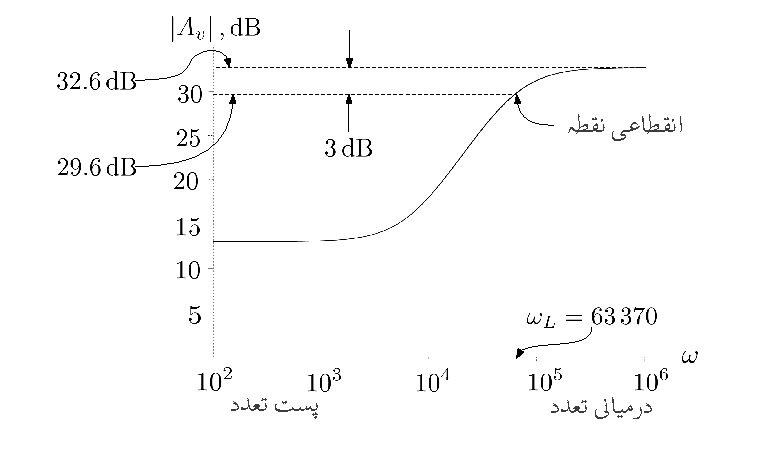
\includegraphics[scale=0.90]{bodePlotWithCE}
\caption{\عددی{C_E} سے حاصل \عددی{\omega_L}}
\label{شکل_مخارج_کپیسٹر_سے_حاصل_پست_انقطاعی_تعدد}
\end{figure}
شکل \حوالہ{شکل_مخارج_کپیسٹر_سے_حاصل_پست_انقطاعی_تعدد} میں \عددی{\abs{A_v}=43 \sqrt{\frac{\omega^2+6666^2}{\omega^2+64068^2}}} کا خط کھینچا گیا ہے جس میں افقی محدد پر \عددی{\log \omega} اور عمودی محدد پر \عددی{20 \log \abs{A_v}} رکھے گئے ہیں۔یوں عمودی محدد سے افزائش کو \اصطلاح{ڈیسی بیل}\حاشیہب{\si{dB}} میں پڑھا جائے گا۔


\انتہا{مثال}
%=========



%====================================
\حصہ{کلکٹر  سرے پر کپیسٹر \عددی{C_C}}
ایمپلیفائر کا خارجی اشارہ کپیسٹر \عددی{C_C} کے ذریعہ حاصل کرنے سے یک سمتی متغیرات متاثر نہیں ہوتے۔شکل \حوالہ{شکل_محاصل_کپیسٹر_کے_اثرات} الف میں کلکٹر  سرے سے \عددی{C_C} کے ذریعہ خارجی اشارے کو درکار مقام یعنی \عددی{R_L} تک پہنچایا گیا ہے۔شکل \حوالہ{شکل_محاصل_کپیسٹر_کے_اثرات} ب میں اسی کا مساوی باریک اشاراتی دور دکھایا گیا۔
\begin{figure}
\centering
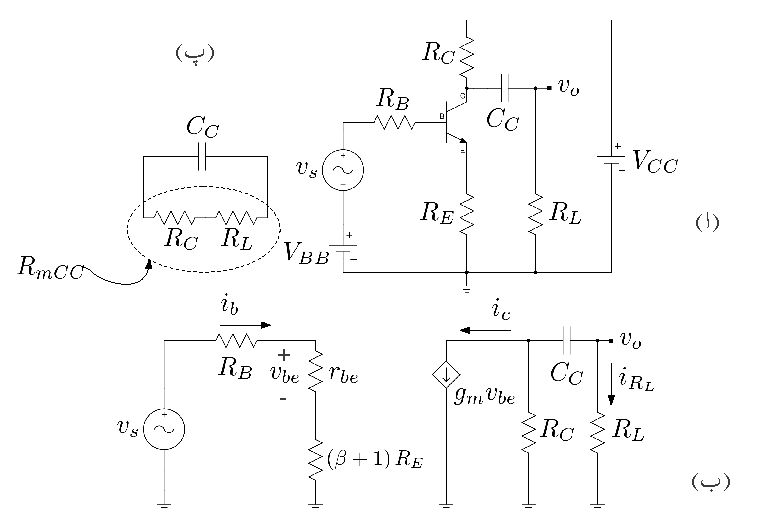
\includegraphics[scale=0.90]{amplifierWithCC}
\caption{کپیسٹر \عددی{C_C} کے اثرات}
\label{شکل_محاصل_کپیسٹر_کے_اثرات}
\end{figure}
سلسلہ وار جڑے \عددی{R_L} اور \عددی{C_C} کا برقی رکاوٹ \عددی{Z}
\begin{align*}
Z=R_L+\frac{1}{s C_C}
\end{align*}
ہے۔برقی رو کے تقسیم کی مساوات سے \عددی{R_C} کے ساتھ متوازی جڑے برقی رکاوٹ \عددی{Z} میں  \عددی{i_{R_L}}  یوں حاصل کیا جائے گا۔
\begin{align*}
i_{R_L}=-\left( \frac{R_C }{R_C+Z} \right) i_c
\end{align*}
جہاں منفی کی علامت اس لئے پیدا ہوئی کہ  \عددی{i_{R_L}} کی سمت \عددی{i_c} کے الٹ رکھی گئی۔
	

افزائش کی مساوات یوں لکھی جائے گی۔ 
\begin{align*}
A_v&=\frac{v_o}{v_s}=\left(\frac{v_o}{i_{R_L}} \right ) \left(\frac{i_{R_L}}{i_c} \right ) \left (\frac{i_c}{v_{be}} \right ) \left (\frac{v_{be}}{v_s} \right )\\
&=\left(R_L \right ) \left(-\frac{R_C}{R_C+Z} \right ) \left(g_m \right ) \left (\frac{r_{be}}{R_S+r_{be}+(\beta+1)R_E} \right )
\end{align*}
منفی کی علامت باہر نکالتے ہوئے، \عددی{\tfrac{R_C}{R_C+Z}} میں \عددی{Z} کی قیمت پر کر کے اسے  دائیں منتقل کرتے ہیں۔
\begin{align*}
A_v&=-\left(R_L \right ) \left(g_m \right ) \left(\frac{r_{be}}{R_S+r_{be}+(\beta+1)R_E} \right ) \left (\frac{R_C}{R_C+R_L+\frac{1}{s C_C}} \right )\\
&=-\left(\frac{R_L g_m r_{be}}{R_S+r_{be}+(\beta+1)R_E} \right ) \left(\frac{s R_C}{\left(R_C+R_L \right ) \left(s+\frac{1}{(R_C+R_L)C_C} \right )} \right )
\end{align*}
جہاں دائیں جانب آخری کسر میں نیچے   \عددی{(R_C+R_L)} باہر نکالا گیا ہے۔اسی کسر کے اوپر حصے سے \عددی{R_C} اور اس کے نیچے   حصے سے \عددی{(R_C+R_L)} کو مساوات کے بائیں جانب منتقل کرتے ہوئے اسے یوں لکھا جا سکتا ہے۔
\begin{gather}
\begin{aligned}
A_v&=-\frac{R_C R_L}{R_C + R_L}  \left(\frac{g_m r_{be}}{R_S+r_{be}+(\beta+1)R_E} \right ) \left(\frac{s}{s+\frac{1}{(R_C + R_L)C_C}} \right )\\
&=A_{vD} \left(\frac{s}{s+\omega_L} \right )
\end{aligned}
\end{gather}
جہاں
\begin{gather}
\begin{aligned}
A_{vD}&=\eval{A_v}_{\omega \to \infty}=-\frac{R_C R_L}{R_C + R_L}   \left(\frac{g_m r_{be}}{R_S+r_{be}+(\beta+1)R_E} \right ) \\
\omega_L&=\frac{1}{(R_C + R_L)C_C}
\end{aligned}
\end{gather}
کے برابر ہیں۔
%=============================
\حصہ{بوڈا خطوط}
ایمپلیفائر کے افزائش بالمقابل تعدد کے خط کو عموماً \اصطلاح{بوڈا خط}\فرہنگ{بوڈا خط}\فرہنگ{Bode plot}\حاشیہب{Bode plot} کے طرز پر کھینچا جاتا ہے\حاشیہد{ہنڈرک واڈ بوڈا نے خط کھینچنے کے اس طرز کو دریافت کیا۔ان خطوط کو بوڈا یا بوڈی خطوط پکارا جاتا ہے}۔افزائش کی حتمی قیمت بالمقابل تعدد اور افزائش کا زاویہ بالمقابل تعدد کے خط علیحدہ علیحدہ کھینچے جاتے ہیں جنہیں \اصطلاح{حتمی قیمت بالمقابل تعدد کا بوڈا خط} اور \اصطلاح{زاویہ بالمقابل تعدد کا بوڈا خط} پکارا جاتا ہے۔\اصطلاح{حتمی قیمت بالمقابل تعدد کے بوڈا خط} میں افقی محدد پر \عددی{\log \omega} یا \عددی{\log f} جبکہ اس کے عمودی محدد پر \عددی{20 \log \abs{A_v}} رکھے جاتے ہیں۔یوں عمودی محدد پر حتمی قیمت \اصطلاح{ڈیسی بیل}\فرہنگ{ڈیسی بیل}\حاشیہب{dB}\فرہنگ{dB} میں پائی جائے گی۔\اصطلاح{زاویہ بالمقابل تعدد کے بوڈا خط} میں افقی محدد پر \عددی{\log \omega} یا \عددی{\log f} جبکہ عمودی محدد پر زاویہ \عددی{\theta} رکھا جاتا ہے۔بوڈا خطوط کو سمجھنے کی خاطر مساوات \حوالہ{مساوات_تعددی_ردعمل_مخارج_کپیسٹر_معیاری_مساوات_الف} کو مثال بناتے ہوئے افزائش کی \اصطلاح{حتمی قیمت بالمقابل تعدد کا بوڈا خط} کھینچتے ہیں۔ مساوات میں
\begin{align*}
A_{vD}&=\SI[per=frac,fraction=nice]{-177.8}{\volt \per \volt} \\
f_1&=\SI{100}{\hertz}\\
f_2&=\SI{10}{\kilo \hertz}
\end{align*}
  لیتے  ہوئے  یہاں دوبارہ پیش کرتے ہیں۔
\begin{align*}
A_v& =A_{vD} \left(\frac{j f +f_1}{j f +f_2} \right)\\
&=A_{vD} \frac{f_1}{f_2}\left(\frac{1+j\frac{f}{f_1}}{1 +j\frac{f}{f_2}} \right)\\
&=-177.8\left( \frac{100}{10000}\right) \left(\frac{1+j\frac{f}{100}}{1+j \frac{f}{10000}}\right)\\
&=-1.778 \left(\frac{1+j\frac{f}{100}}{1+j \frac{f}{10000}}\right)\\
&=\abs{A_{v}} e^{j \theta}
\end{align*}
جہاں
\begin{gather}
\begin{aligned} \label{مساوات_تعددی_ردعمل_بوڈا_جزو_مثال}
\abs{A_v}&=1.778  \frac{\sqrt{1+\left(\frac{f}{100} \right)^2}}{\sqrt{1+\left(\frac{f}{10000}\right)^2}} \\
\theta &=\pi+\left(\tan^{-1} \frac{f}{100} \right)-\left(\tan^{-1} \frac{f}{10000} \right)
\end{aligned}
\end{gather}
کے برابر ہیں۔ آئیں مساوات \حوالہ{مساوات_تعددی_ردعمل_بوڈا_جزو_مثال} کو استعمال کرتے ہوئے  \عددی{\abs{A_v}} بالمقابل \عددی{f} کا بوڈا خط کھینچنا سیکھیں۔

\عددی{\abs{A_v}} کو \اصطلاح{ڈیسی بیل}\حاشیہب{decibell} میں لکھتے ہوئے
\begin{align} \label{مساوات_تعددی_ردعمل_بوڈا_خط_حیطہ}
\abs{A_v}_{dB}=20 \log  1.778  +20 \log \sqrt{1+\frac{f^2}{100^2}} -20 \log \sqrt{1+\frac{f^2}{10000^2}} 
\end{align} 
حاصل ہوتا ہے۔\عددی{\abs{A_v}_{dB}} کا خط کھینچنے کی خاطر مندرجہ بالا مساوات کے تین اجزاء کے خطوط کو باری باری کھینچتے ہوئے آخر میں تمام کا سادہ مجموعہ حاصل کریں گے۔
\begin{figure}
\centering
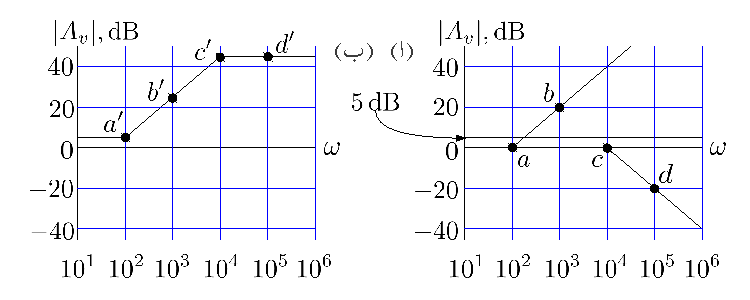
\includegraphics[scale=0.90]{bodeMagnitudeAandB}
\caption{حتمی قیمت بالمقابل تعدد کے بوڈا خط کے اجزاء}
\label{شکل_تعددی_ردعمل_بوڈا_اجزاء_الف}
\end{figure}

ایسا کرنے کی خاطر مساوات \حوالہ{مساوات_تعددی_ردعمل_بوڈا_خط_حیطہ} کو دیکھتے ہیں۔اس کا پہلا جزو
\begin{align*}
20 \log 1.778 \approx \SI{5}{dB}
\end{align*}
 ایک مستقل مقدار ہے جس کی قیمت تعدد پر منحصر نہیں۔اس  سے  \عددی{\SI{5}{dB}} پر سیدھا افقی خط  حاصل ہوتا ہے جسے شکل \حوالہ{شکل_تعددی_ردعمل_بوڈا_اجزاء_الف} الف میں دکھایا گیا ہے۔

مساوات کے دوسرے جزو کی کارکردگی نہایت کم اور نہایت زیادہ تعدد پر دیکھتے ہیں۔نہایت کم تعدد یعنی \عددی{f \ll f_1} پر چونکہ \عددی{\left(\tfrac{f}{f_1} \right)^2 \ll 1} ہو گا لہٰذا اس جزو سے
\begin{align} \label{مساوات_تعدد_ردعمل_بوڈا_کم_تعدد_حصہ}
20 \log  \sqrt{1+\left(\frac{f}{f_1}\right)^2}  \to 20 \log 1 =\SI{0}{dB}
\end{align}
حاصل ہوتا ہے۔نہایت زیادہ یعنی \عددی{f \gg f_1} پر چونکہ \عددی{\left(\tfrac{f}{f_1} \right)^2 \gg 1} ہو گا لہٰذا
\begin{align} \label{مساوات_تعدد_ردعمل_بوڈا_زیادہ_تعدد_حصہ}
20 \log  \sqrt{1+\left(\frac{f}{f_1}\right)^2} \to 20 \log \sqrt{\left(\frac{f}{f_1}\right)^2} =20 \log \frac{f}{100} \hspace{1 cm} \SI{}{dB}
\end{align}
حاصل ہوتا ہے جہاں آخری قدم پر \عددی{f_1=100} کا استعمال کیا گیا ہے۔

\عددی{20 \log \frac{f}{100}} کی قیمت \عددیء{100}، \عددیء{1000}، \عددی{10000} اور \عددی{100000} کے تعدد پر \عددیء{0}، \عددیء{20}، \عددی{40} اور \عددی{60} ڈیسی بیل حاصل ہوتی ہے۔اس حقیقت کو یوں بیان کیا جا سکتا ہے کہ تعدد دس گنّا کرنے سے افزائش \عددی{\SI{20}{dB}} بڑھتی ہے یا کہ افزائش  \عددی{\SI{20}{dB}} فی دہائی کے شرح سے بڑھتی ہے۔ افقی محور پر تعدد کا لوگارتھم لیتے ہوئے ان قیمتوں کے استعمال سے خط کھینچا گیا ہے۔یہ خط تعدد کے محور کو \عددی{f_1} یعنی \عددی{\log(100)=2} پر چھوتے ہوئے \عددی{\SI{20}{dB}} فی دہائی کے شرح سے بڑھتا ہے۔ایسا خط کھینچتے وقت \عددی{(f_1, \SI{0}{dB})}  اور  \عددی{(10 f_1, \SI{20}{dB})} کے مقام پر نقطے  لگا کر انہیں سیدھی لکیر سے جوڑتے ہوئے حاصل کیا جاتا ہے۔

شکل \حوالہ{شکل_تعددی_ردعمل_بوڈا_اجزاء_الف} الف میں \عددی{(f_1, \SI{0}{dB})} یعنی \عددی{(10^2, \SI{0}{dB})} پر نقطہ \عددی{a} اور اسی طرح \عددی{(10 f_1, \SI{20}{dB})} یعنی \عددی{(10^3,\SI{20}{dB})} پر نقطہ \عددی{b} دکھائے گئے ہیں۔نہایت کم تعدد پر مساوات \حوالہ{مساوات_تعدد_ردعمل_بوڈا_کم_تعدد_حصہ} کے مطابق اس جزو کی قیمت \عددی{\SI{0}{dB}} ہے۔حقیقت میں بوڈا خط کھینچتے وقت کم تعدد کو \عددی{f \ll f_1} کی بجائے \عددی{f \le f_1} لیا جاتا ہے۔یوں نقطہ \عددی{a} سے کم تعدد پر اس جزو کی قیمت \عددی{\SI{0}{dB}} دکھائی گئی ہے۔اس طرح بوڈا خط کھینچتے ہوئے  نہایت زیادہ تعدد کو \عددی{f \gg f_1} کی بجائے \عددی{f \ge f_1} لیا جاتا ہے۔ یوں اگر \عددی{a} پر \عددی{\SI{0}{dB}} ہو تب دس گنا زیادہ تعدد پر \عددی{\SI{20}{dB}} ہو گا۔اس نقطے  کو \عددی{b} سے ظاہر کیا گیا ہے۔\عددی{a} تک \عددی{\SI{0}{dB}} پر رہتا ہوا اور \عددی{a} اور \عددی{b} سے گزرتا سیدھا خط دوسرے جزو کا \اصطلاح{بوڈا خط} ہے۔


مساوات \حوالہ{مساوات_تعددی_ردعمل_بوڈا_خط_حیطہ} کے تیسرے جزو  کی کارکردگی نہایت کم اور نہایت زیادہ تعدد پر دیکھتے ہیں۔نہایت کم تعدد یعنی \عددی{f \ll f_2} پر
\begin{align} \label{مساوات_تعدد_ردعمل_بوڈا_کم_تعدد_تیسرا_حصہ}
-20 \log \sqrt{1+\left(\frac{f}{f_2}\right)^2} \to 20 \log 1 =\SI{0}{dB}
\end{align}
جبکہ نہایت زیادہ تعدد یعنی \عددی{f \gg f_2} پر 
\begin{gather}
\begin{aligned} \label{مساوات_تعدد_ردعمل_بوڈا_زیادہ_تعدد_تیسرا_حصہ}
-20 \log  \sqrt{1+\left(\frac{f}{f_2}\right)^2} &\to -20 \log \sqrt{\left(\frac{f}{f_2}\right)^2} \\
&=-20 \log \frac{f}{10000} \hspace{1 cm} \SI{}{dB}
\end{aligned}
\end{gather}
حاصل ہوتا ہے  جہاں آخری قدم پر \عددی{f_2=10000} کا استعمال کیا گیا ہے۔

\عددی{-20 \log \frac{f}{10000}} کی قیمت \عددیء{10000}، \عددیء{100000}، \عددی{1000000} اور \عددی{10000000} کے تعدد پر \عددیء{0}، \عددیء{-20}، \عددی{-40} اور \عددی{-60} ڈیسی بیل حاصل ہوتی ہے۔اس حقیقت کو یوں بیان کیا جا سکتا ہے کہ تعدد دس گنّا کرنے سے افزائش \عددی{\SI{20}{dB}} گھٹتی ہے یا کہ افزائش  \عددی{\SI{-20}{dB}} فی دہائی کے شرح سے تبدیل ہوتی ہے۔ افقی محور پر تعدد کا لوگارتھم لیتے ہوئے ان قیمتوں کے استعمال سے خط کھینچا گیا ہے۔یہ خط تعدد کے محور کو \عددی{f_2} یعنی \عددی{\log(10000)=4} پر چھوتے ہوئے \عددی{\SI{-20}{dB}} فی دہائی کے شرح سے تبدیل ہوتا ہے۔ایسا خط کھینچتے وقت \عددی{f_2} تعدد پر \عددی{\SI{0}{dB}} اور \عددی{10 f_2} تعدد پر \عددی{\SI{-20}{dB}}  کے مقام پر نقطے  لگا کر انہیں سیدھی لکیر سے جوڑتے ہوئے حاصل کیا جاتا ہے۔شکل \حوالہ{شکل_تعددی_ردعمل_بوڈا_اجزاء_الف} الف  میں ان نقطوں کو \عددی{c} اور \عددی{d} سے ظاہر کیا گیا ہے۔یاد رہے کہ \عددی{f_2} یعنی \عددی{10^4} سے کم تعدد پر اس جزو کی قیمت \عددی{\SI{0}{dB}} ہے۔

شکل \حوالہ{شکل_تعددی_ردعمل_بوڈا_اجزاء_الف} ب میں ان تینوں خطوط کا مجموعہ لیا گیا ہے جو کہ مساوات  \حوالہ{مساوات_تعددی_ردعمل_بوڈا_جزو_مثال} کے \عددی{\abs{A_v}} کا مکمل \اصطلاح{بوڈا خط} ہے۔شکل \حوالہ{شکل_تعددی_ردعمل_بوڈا_اجزاء_الف} الف میں نقطہ \عددی{a} پر  مساوات \حوالہ{مساوات_تعددی_ردعمل_بوڈا_خط_حیطہ} کے پہلے جزو کے خط کی قیمت \عددی{\SI{5}{dB}} جبکہ بقایا دو اجزاء کے قیمتیں \عددی{\SI{0}{dB}} ہیں۔یوں ان کا مجموعہ \عددی{\SI{5}{dB}} ہے جسے شکل \حوالہ{شکل_تعددی_ردعمل_بوڈا_اجزاء_الف} ب میں  \عددی{a'} سے ظاہر کیا گیا ہے۔\عددی{b} پر ان تین اجزاء کے قیمتیں \عددیء{\SI{5}{dB}}، \عددی{\SI{20}{dB}} اور \عددی{\SI{0}{dB}} ہیں جن کے مجموعہ \عددی{\SI{25}{dB}} کو \عددی{b'} سے ظاہر کیا گیا ہے۔\عددی{c} پر تینوں کا مجموعہ \عددی{\SI{45}{dB}} کو \عددی{c'} سے ظاہر کیا گیا ہے۔\عددی{d} پر تین اجزاء کے قیمتیں \عددیء{\SI{5}{dB}}، \عددی{\SI{60}{dB}} اور \عددی{\SI{-20}{dB}} ہیں جن کا مجموعہ \عددی{\SI{45}{dB}} ہی ہے۔اس نقطے  کو \عددی{d'} سے ظاہر کیا گیا ہے۔

مندرجہ بالا تمام عمل کو نہایت آسانی سے یوں سرانجام دیا جا سکتا ہے۔دئے گئے مساوات کی حتمی قیمت کمتر تعدد پر  حاصل کریں۔بوڈا خط کی قیمت یہی رکھتے ہوئے تعدد بڑھائیں حتٰی کہ مساوات کا \اصطلاح{صفر} یا \اصطلاح{قطب} آ جائے۔اگر \اصطلاح{صفر} آ جائے تو بوڈا خط کی قیمت \عددی{\SI{20}{dB}} فی دہائی کی شرح سے بڑھانا شروع کر دیں اور اگر \اصطلاح{قطب} آ جائے تو بوڈا خط کی قیمت \عددی{\SI{20}{dB}} فی دہائی کی شرح سے گھٹانا شروع کر دیں۔تعدد بڑھاتے رہیں حتٰی کہ مساوات کا اگلا \اصطلاح{صفر} یا \اصطلاح{قطب} آ جائے۔ہر مرتبہ \اصطلاح{صفر} آنے پر بوڈا خط کے تبدیلی کی شرح میں \عددی{\SI{20}{dB}} کا اضافہ لائیں جبکہ \اصطلاح{قطب} آنے پر بوڈا خط کے تبدیلی کی شرح میں \عددی{\SI{20}{dB}} کی کمی لائیں۔
\begin{figure}
\centering
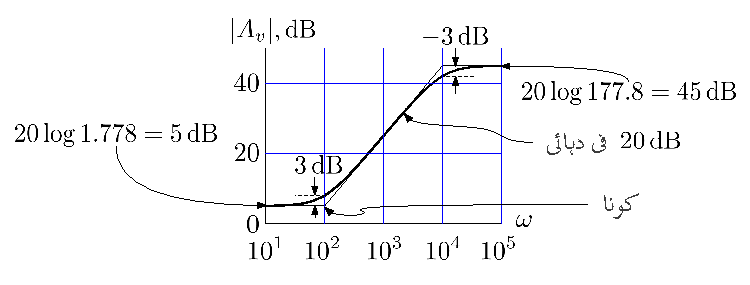
\includegraphics[scale=0.90]{bodeMagnitudeC}
\caption{اصل خط اور بوڈا خط کا موازنہ}
\label{شکل_تعددی_ردعمل_بوڈا_اصل_موازنہ}
\end{figure}

شکل \حوالہ{شکل_تعددی_ردعمل_بوڈا_اصل_موازنہ} میں مساوات \حوالہ{مساوات_تعددی_ردعمل_بوڈا_جزو_مثال} کے بوڈا خط اور اس کا حقیقی خط\حاشیہد{حقیقی خط کمپیوٹر کے پروگرام میٹ لیب matlab یا آقٹیو octave  کی مدد سے باآسانی کھینچا جا سکتا ہے۔اس کتاب میں بیشتر خطوط لینکس linux میں پائے جانے والے پروگرام آقٹیو استعمال کرتے ہوئے ہی کھینچے گئے ہیں۔} ایک ساتھ دکھائے گئے ہیں۔آپ دیکھ سکتے ہیں کہ بوڈا خط کے کونوں پر دونوں خطوط میں \عددی{\SI{3}{dB}} کا فرق پایا جاتا ہے جبکہ بقایا تعدد پر دونوں تقریباً ایک ہی طرح کے ہیں۔مساوات \حوالہ{مساوات_تعدد_ردعمل_بوڈا_کم_تعدد_حصہ} سے اس فرق کو سمجھا جا سکتا ہے۔ کونے پر تعدد \عددی{f_1} کے برابر ہے یوں اس مساوات سے
\begin{align*}
20 \log \sqrt{1+\left(\frac{f_1}{f_1}\right)^2} = 20 \log \sqrt{2} \approx \SI{3}{dB}
\end{align*}
حاصل ہوتا ہے نا کہ \عددی{\SI{0}{dB}}۔اسی حقیقت کے بنا پر بوڈا خط کے کونوں کو \عددی{\SI{3}{dB}} نقطے  بھی کہتے ہیں۔
 
%==================
\ابتدا{مثال}
مساوات \حوالہ{مساوات_تعددی_ردعمل_مخارج_کپیسٹر} کا بوڈا خط کھینچیں۔

حل:اس مساوات کو دوبارہ پیش کرتے ہیں۔
\begin{align*}
A_v&=-43 \left(\frac{j \omega+6666}{j \omega+64068} \right)
\end{align*}
انتہائی کم تعدد \عددی{(\omega \to 0)} پر اس کی حتمی قیمت
\begin{align*}
\abs{A_v}_{\omega \to 0}&=43 \left(\frac{0+6666}{0+64068} \right)=4.474
\end{align*}
یعنی
\begin{align*}
20 \times \log 4.474 \approx \SI{13}{dB}
\end{align*}
حاصل ہوتی ہے۔مساوات کا \اصطلاح{صفر} \عددی{\num{6666}} جبکہ اس کا \اصطلاح{قطب} \عددی{\num{64068}} پر پایا جاتا ہے۔ان معلومات سے شکل \حوالہ{شکل_تعددی_ردعمل_بوڈا_مخارج_کپیسٹر} میں بوڈا خط حاصل کیا گیا ہے۔
\begin{figure}
\centering
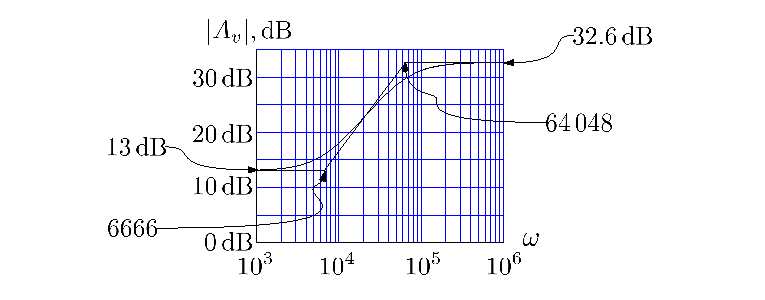
\includegraphics[scale=0.90]{bodeMagnitudeEmitterCapacitor}
\caption{}
\label{شکل_تعددی_ردعمل_بوڈا_مخارج_کپیسٹر}
\end{figure}
\انتہا{مثال}
%==================
\ابتدا{مثال}
مندرجہ ذیل مساوات کا بوڈا خط کھینچیں۔
\begin{align*}
A_v=\frac{1000 s}{s+10}
\end{align*}

حل:اس کو عمومی طرز پر لکھتے ہیں۔
\begin{align*}
A_v&=\frac{100 j \omega}{\frac{j \omega}{10}+1}
\end{align*}
جسے ڈیسی بیل میں لکھتے ملتا ہے
\begin{align*}
A_v&=20 \log 100 +20 \log \omega-20 \log \sqrt{\frac{\omega^2}{10^2}+1}
\end{align*}
اس کے بوڈا خط کے اجزاء شکل \حوالہ{شکل_تعددی_ردعمل_تعددی_جزو} الف جبکہ مکمل بوڈا خط شکل  ب میں دکھائے گئے ہیں۔
\begin{figure}
\centering
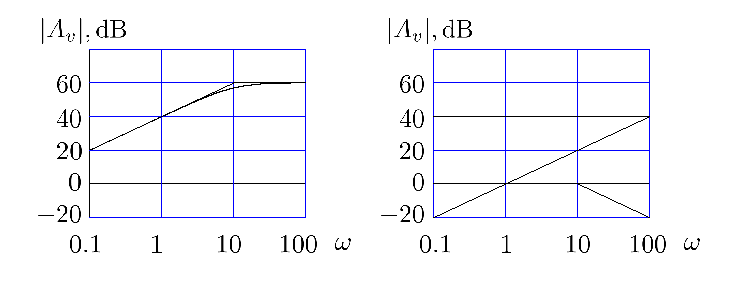
\includegraphics[scale=0.90]{bodeMagnitudeFrequencyTermA}
\caption{}
\label{شکل_تعددی_ردعمل_تعددی_جزو}
\end{figure}
\انتہا{مثال}
%================

مندرجہ بالا مثال میں دی گئی مساوات میں کسر کے اوپر تعددی جزو پر غور کریں۔بوڈا خط میں \عددی{\left(\tfrac{j \omega}{\omega_0}+1 \right)} طرز پر لکھے گئے جزو کی قیمت \عددی{\omega_0} سے کم تعدد پر \عددی{\SI{0}{dB}} جبکہ اس سے زیادہ تعدد پر بیس ڈیسی بیل فی دہائی کی شرح سے تبدیل ہوتا ہے۔اس کے برعکس \عددی{\left(j \omega \right)} کہیں بھی \عددی{\SI{0}{dB}} پر برقرار نہیں رہتا۔یہ \عددی{\omega=1} پر \عددی{\SI{0}{dB}} سے گزرتے ہوئے بیس ڈیسی بیل فی دہائی کی شرح سے تمام تعدد پر تبدیل ہوتا ہے۔اگر یہ جزو بطور \اصطلاح{صفر} پایا جائے تب یہ بیس ڈیسی بیل فی دہائی کی شرح سے بڑھتا ہے جبکہ اگر جزو بطور \اصطلاح{قطب} پایا جائے تب یہ بیس ڈیسی بیل فی دہائی کی شرح سے گھٹتا ہے۔
%=================
\حصہ{بیس  اور کلکٹر  بیرونی کپیسٹر}
شکل \حوالہ{شکل_تعددی_ردعمل_قابو_حاصل_کپیسٹر} میں بیس  اور کلکٹر  پر کپیسٹر نسب کئے گئے ہیں۔اگرچہ شکل میں ایمٹر پر \عددی{C_E} بھی  نسب ہے لیکن اس کی قیمت لامحدود تصور کی گئی ہے۔یوں درکار تعدد پر اس کو قصر دور تصور کیا گیا ہے۔مساوی شکل میں
\begin{figure}
\centering
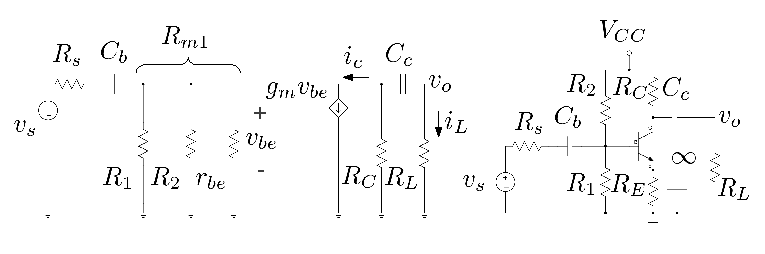
\includegraphics[scale=0.90]{baseCollectorCapacitor}
\caption{بیس  اور کلکٹر  پر کپیسٹر نسب کرنے کے اثرات}
\label{شکل_تعددی_ردعمل_قابو_حاصل_کپیسٹر}
\end{figure}
%
\begin{align*}
\frac{1}{R_{m1}}=\frac{1}{R_1}+\frac{1}{R_2}+\frac{1}{r_{be}}
\end{align*}
لیتے ہوئے ہم لکھ سکتے ہیں۔
\begin{align*}
A_v&=\frac{v_o}{v_s}=\left(\frac{v_o}{i_L}\right) \left(\frac{i_L}{i_c}\right) \left( \frac{i_c}{v_{be}}\right) \left( \frac{v_{be}}{v_s} \right)\\
&=R_L \left(-\frac{R_C}{R_C+R_L+\frac{1}{sC_c}} \right) \left(g_m \right) \left(\frac{R_{m1}}{R_s+R_{m1}+\frac{1}{s C_b}}\right)\\
&=-g_m R_L R_C R_{m1} \left(\frac{sC_c}{sC_c \left(R_C+R_L\right)+1}\right) \left(\frac{sC_b}{sC_b \left(R_s+R_{m1} \right)+1} \right)\\
&=-\frac{g_m R_L R_C R_{m1}}{\left(R_C+R_L \right)\left(R_s+R_{m1} \right)}\left(\frac{s}{s+\frac{1}{C_c \left(R_C+R_L\right)}} \right)\left(\frac{s}{s+\frac{1}{C_b \left(R_s+R_{m1} \right)}} \right)
\end{align*} 
اس مساوات میں
\begin{gather}
\begin{aligned}\label{مساوات_تعددی_ردعمل_قابو_محاصل_کپیسٹر_سادہ_مساوات}
\omega_c&=\frac{1}{C_c \left(R_C+R_L \right)}\\
\omega_b&=\frac{1}{C_b \left(R_s+R_{m1} \right)}
\end{aligned}
\end{gather}
لیتے ہوئے یوں لکھا جا سکتا ہے۔
\begin{align}
A_v&=-\frac{g_m R_L R_C R_{m1}}{\left(R_C+R_L \right)\left(R_s+R_{m1} \right)}\left(\frac{s}{s+\omega_c} \right)\left(\frac{s}{s+\omega_b} \right)
\end{align}
اس مساوات میں \عددی{\frac{R_C R_L}{R_C+R_L}} متوازی جڑے مزاحمت کی کل مزاحمت ہے جسے عموماً \عددی{\mathbin{R_C \| R_L}} لکھا جاتا ہے ۔اسی طرح \عددی{\frac{R_{m1}}{R_{m1+R_s}}} کو \عددی{\frac{1}{R_s} \left(\frac{R_s R_{m1}}{R_s+R_{m1}} \right)} یا \عددی{\tfrac{\mathbin{R_s \| R_{m1}}}{R_S}}لکھتے ہوئے اسے یوں لکھا جا سکتا ہے۔
\begin{gather}
\begin{aligned}\label{مساوات_تعددی_ردعمل_قابو_محاصل_کپیسٹر}
A_v&=-\frac{1}{R_s} \left(\mathbin{R_C \| R_L} \right) \left( \mathbin{R_s \| R_{m1}}\right)\left(\frac{s}{s+\omega_c} \right)\left(\frac{s}{s+\omega_b} \right)\\
&=A_{vD}\left(\frac{s}{s+\omega_c} \right)\left(\frac{s}{s+\omega_b} \right)
\end{aligned}
\end{gather}
جہاں
\begin{align*}
A_{vD}=-\frac{1}{R_s} \left(\mathbin{R_C \| R_L} \right) \left( \mathbin{R_s \| R_{m1}}\right)
\end{align*}
لکھا گیا ہے۔

پست انقطاعی تعدد پر \عددی{\abs{A_v}=\tfrac{A_{vD}}{\sqrt{2}}} کے برابر ہو گا۔یوں مساوات \حوالہ{مساوات_تعددی_ردعمل_قابو_محاصل_کپیسٹر} میں پست انقطاعی تعدد کو \عددی{\omega_L} لکھتے ہوئے حاصل ہوتا ہے
\begin{align*}
A_{vD} \left(\frac{\omega_L}{\sqrt{\omega_L^2+\omega_c^2}} \right)\left(\frac{\omega_L}{\sqrt{\omega_L^2+\omega_b^2}} \right)=\frac{A_{vD}}{\sqrt{2}}
\end{align*}
جسے
\begin{align*}
2 \omega_L^4=\left(\omega_L^2+\omega_c^2 \right)\left(\omega_L^2+\omega_b^2\right)
\end{align*}
یعنی
\begin{align*}
\omega_L^4-\left(\omega_c^2+\omega_b^2 \right) \omega_L^2 -\omega_c^2 \omega_b^2=0
\end{align*}
لکھا جا سکتا ہے۔اس کو حل کرتے ملتا ہے
\begin{align}\label{مساوات_تعددی_ردعمل_قابو_محاصل_کپیسٹر_انقطاعی_تعدد}
\omega_L^2=\frac{\omega_c^2+\omega_b^2}{2}+\frac{\sqrt{\omega_c^4+6 \omega_c^2 \omega_b^2+\omega_b^4}}{2}
\end{align}
مندرجہ بالا مساوات میں منفی  جزر  کو شامل نہیں کیا گیا چونکہ اس کے استعمال سے \عددی{\omega_L^2} کی قیمت منفی حاصل ہوتی ہے۔

شکل \حوالہ{شکل_تعددی_ردعمل_قابو_حاصل_کپیسٹر} کو دیکھ کر معلوم ہوتا ہے کہ \عددی{C_b} اور \عددی{C_c} کا ایک دوسرے پر کوئی اثر نہیں۔ مساوات \حوالہ{مساوات_تعددی_ردعمل_قابو_محاصل_کپیسٹر} اسی حقیقت کی تصدیق کرتا ہے۔
%==================
\ابتدا{مثال}\شناخت{مثال_تعددی_ردعمل_قابو_محاصل_کپیسٹر_دور_کونے}
شکل \حوالہ{شکل_تعددی_ردعمل_قابو_حاصل_کپیسٹر} میں
\begin{align*}
V_{CC}=\SI{9}{\volt}, R_C=\SI{1.8}{\kilo \ohm}, R_E=\SI{200}{\ohm}\\
R_1=\SI{2.2}{\kilo \ohm}, R_2=\SI{16}{\kilo \ohm}, R_s=\SI{1}{\kilo \ohm}\\
\beta=\num{99}, R_L=\SI{1.8}{\kilo \ohm}
\end{align*}
ہیں۔
\begin{itemize}
\item
\عددی{C_b} اور \عددی{C_c} کی ایسی قیمتیں حاصل کریں کہ \عددی{f_b=\SI{50}{\hertz}} جبکہ  \عددی{f_c=\SI{5}{\hertz}} ہو۔
\item
مندرجہ بالا قیمتوں کو استعمال کرتے ہوئے  مساوات \حوالہ{مساوات_تعددی_ردعمل_قابو_محاصل_کپیسٹر} کا بوڈا خط کھینچتے ہوئے  پست انقطاعی تعدد حاصل کریں۔
\item
\عددی{f_b=f_c} رکھتے ہوئے پست انقطاعی تعدد \عددی{\SI{50}{\hertz}} حاصل کرنے کی خاطر \عددی{f_b} اور \عددی{f_c} حاصل کریں
\end{itemize}

حل:
نقطہ کارکردگی حاصل کرتے وقت تمام کپیسٹر کھلے سرے کردار ادا کرتے ہیں۔مسئلہ تھونن کی مدد سے \عددی{R_{th}=\SI{1.934}{\kilo \ohm}} جبکہ \عددی{V_{th}=\SI{1.0879}{\volt}} حاصل ہوتے ہیں جن سے \عددیء{I_{CQ}=\SI{1.768}{\milli \ampere}}، \عددی{g_m=\SI{0.071}{\siemens}} اور \عددی{r_{be}=\SI{1.394}{\kilo \ohm}} حاصل ہوتے ہیں۔یوں \عددی{R_{m1}=\SI{810}{\ohm}} حاصل ہوتا ہے۔
\begin{itemize}
\item
\begin{align*}
C_c=\frac{1}{2 \pi f_c \left(R_C+R_L \right) }=\frac{1}{2 \times \pi \times 5 \times \left(1800+1800 \right)}=\SI{8.84}{\micro \farad}\\
C_b=\frac{1}{2 \pi f_b \left(R_s+R_{m1} \right) }=\frac{1}{2 \times \pi \times 50 \times \left(1000+810 \right)}=\SI{1.76}{\micro \farad}
\end{align*}
%
\item
%
\begin{figure}
\centering
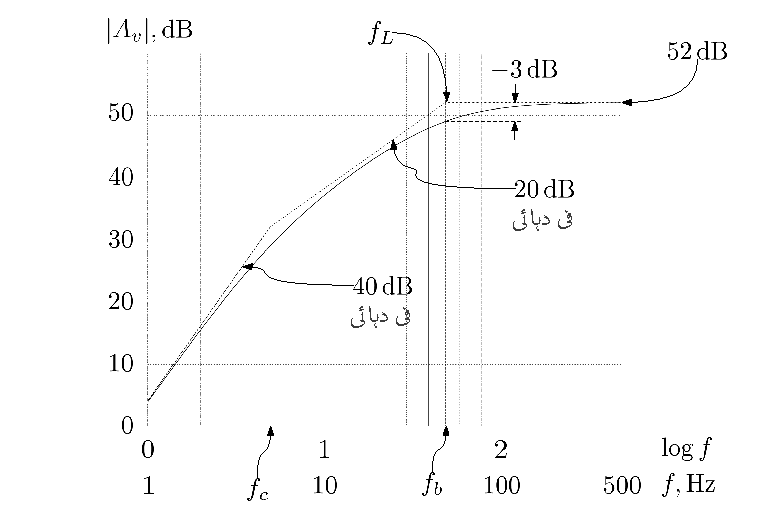
\includegraphics[scale=0.90]{bodeMagnitudeBaseAndCollectorCapacitor}
\caption{پست انقطاعی نقطہ زیادہ تعدد والے کونے پر ہے}
\label{شکل_تعددی_ردعمل_قابو_کپیسٹر_پست_انقطاعی_تعین}
\end{figure}
شکل \حوالہ{شکل_تعددی_ردعمل_قابو_کپیسٹر_پست_انقطاعی_تعین} میں بوڈا خط کھینچا گیا ہے جہاں سے واضح ہے کہ پست انقطاعی تعدد تقریباً \عددی{f_b} کے برابر ہے۔شکل میں \عددی{\SI{1}{\hertz}} تا \عددی{\SI{5}{\hertz}} بوڈا خط کی ڈھلوان \عددی{\SI{40}{dB}} فی دہائی ہے جبکہ \عددی{\SI{5}{\hertz}} تا \عددی{\SI{50}{\hertz}} اس کی ڈھلوان \عددی{\SI{20}{dB}} فی دہائی ہے۔

جب بھی بوڈا خط میں پست انقطاعی نقطہ تعین کرنے والے کونوں میں سب سے زیادہ تعدد پر پائے جانے والے کونے سے بقایا کونے دور دور ہوں، ایسی صورت میں پست انقطاعی نقطہ تقریباً اسی زیادہ تعدد کے کونے پر ہو گا۔

آئیں مساوات \حوالہ{مساوات_تعددی_ردعمل_قابو_محاصل_کپیسٹر_انقطاعی_تعدد} حل کرتے دیکھیں کہ جواب کیا حاصل ہوتا ہے۔اس مساوات میں \عددی{\omega_c} اور \عددی{\omega_b} کی قیمتیں پر کرتے ملتا ہے
\begin{align*}
\omega_L&=\num{317.254}\\
f_L&=\SI{50.49}{\hertz}
\end{align*}
%
\item
مساوات \حوالہ{مساوات_تعددی_ردعمل_قابو_محاصل_کپیسٹر_انقطاعی_تعدد} میں \عددی{\omega_c=\omega_b} پُر کرتے حل کرتے ہیں
\begin{align*}
\omega_L^2=\frac{2 \omega_b^2+\sqrt{\omega_b^4+6 \omega_b^4+\omega_b^4}}{2}=\left(1+\sqrt{2} \right)\omega_b^2
\end{align*}
یوں
\begin{align*}
\omega_L=\left(\sqrt{1+\sqrt{2}}\right)\omega_b
\end{align*}
حاصل ہوتا ہے جس سے \عددی{f_L=\SI{50}{\hertz}} حاصل کرنے کی خاطر
\begin{align*}
f_b=\frac{f_L}{\sqrt{1+\sqrt{2}}}=\frac{50}{\sqrt{1+\sqrt{2}}}=\SI{32}{\hertz}
\end{align*}
رکھنا ہو گا۔شکل \حوالہ{شکل_تعددی_ردعمل_قابو_کپیسٹر_پست_انقطاعی_تعین_الف} میں صورت حال دکھایا گیا ہے۔
\begin{figure}
\centering
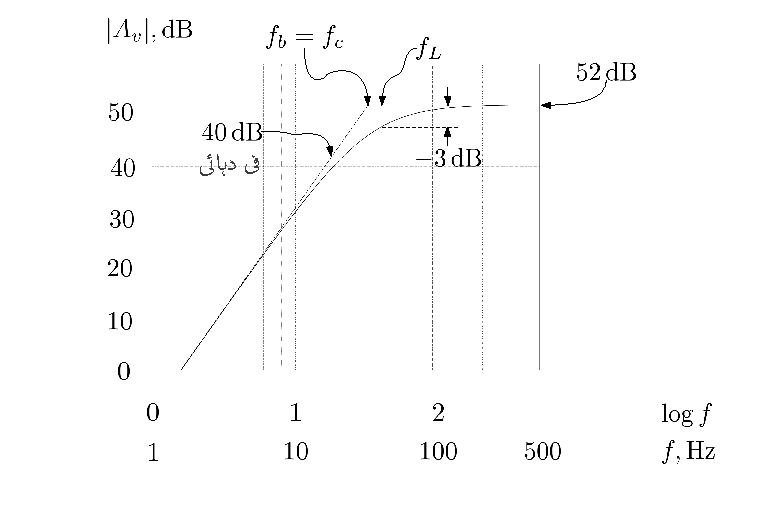
\includegraphics[scale=0.90]{bodeMagnitudeBaseAndCollectorCapacitorA}
\caption{جڑوا کونوں کی صورت میں پست انقطاعی نقطہ}
\label{شکل_تعددی_ردعمل_قابو_کپیسٹر_پست_انقطاعی_تعین_الف}
\end{figure}
\end{itemize}
\انتہا{مثال}
%=================
\حصہ{بیس  اور ایمٹر بیرونی کپیسٹروں کا مجموعی اثر}
اب تک دیکھے گئے تمام ادوار میں ہم نے دیکھا کہ کسی بھی کپیسٹر کی بدولت پیدا بوڈا خط کے \اصطلاح{قطب} کو \عددی{\omega=\tfrac{1}{R_m C}} لکھا جا سکتا تھا جہاں \عددی{R_m} اس کپیسٹر کے متوازی جڑی مزاحمت ہے۔بیس  اور ایمٹر دونوں پر کپیسٹر نسب کرنے سے ایسا سادہ مساوات حاصل نہیں ہوتا۔آئیں شکل \حوالہ{شکل_تعددی_رد_عمل_قابو_مخارج_کپیسٹر_الف} میں \عددی{\tfrac{v_L}{v_i}} حاصل کرتے ہوئے اس صورت کو بھی دیکھیں۔
\begin{figure}
\centering
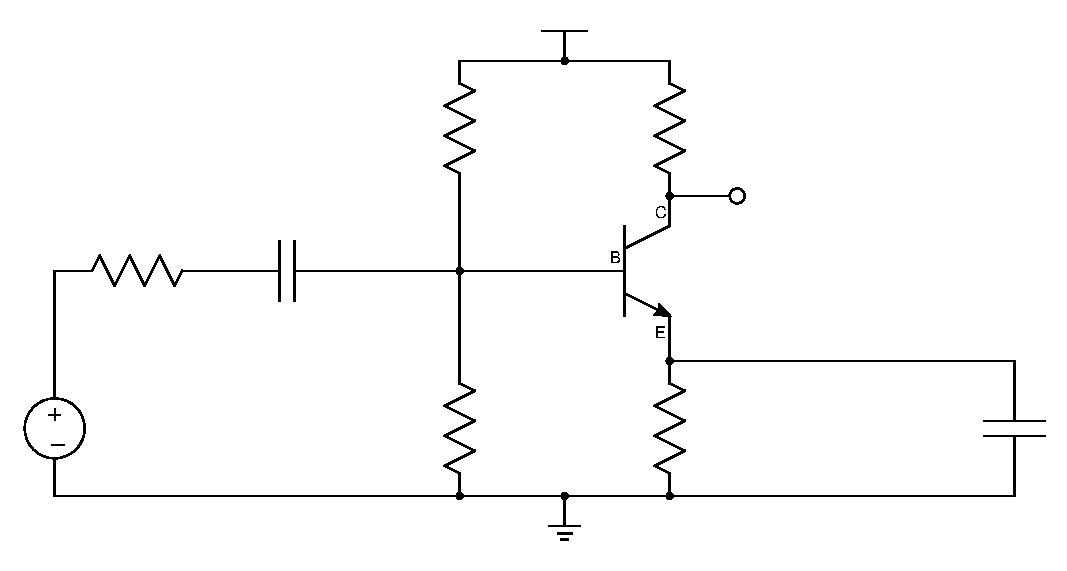
\includegraphics[scale=0.90]{commonEmitterCbCeLowCutoffFrequencyA}
\caption{}
\label{شکل_تعددی_رد_عمل_قابو_مخارج_کپیسٹر_الف}
\end{figure}
%
شکل \حوالہ{شکل_تعددی_رد_عمل_قابو_مخارج_کپیسٹر_ب} میں اس کا باریک مساوی دور دکھایا گیا ہے جس میں \عددی{R_e} اور \عددی{C_e} کو ٹرانزسٹر کے بیس  جانب منتقل کرتے ہوئے \عددی{R_e'} اور \عددی{C_e'} لکھا گیا ہے۔یوں
\begin{align*}
R_e' &=\left(\beta+1 \right) R_e\\
C_e'&=\frac{C_e}{\beta+1}
\end{align*}
ہیں۔شکل کو دیکھتے ہوئے ہم لکھ سکتے ہیں
\begin{gather}
\begin{aligned}\label{مساوات_تعددی_ردعمل_قابو_مخارج_کپیسٹر}
A_v&=\frac{v_L}{v_i}=\frac{v_L}{i_c} \times \frac{i_c}{i_b} \times \frac{i_b}{v_b} \times \frac{v_b}{v_i}\\
&=-R_c \beta \left(\frac{1}{R_e'}+s C_e' \right) \left(\frac{Z}{r_i+\frac{1}{sC_b}+Z} \right)
\end{aligned}
\end{gather}
جہاں \عددی{r_{be}} کو نظر انداز کرتے ہوئے
\begin{align*}
\frac{1}{Z}=\frac{1}{R_1}+\frac{1}{R_2}+\frac{1}{R_e'}+s C_e'
\end{align*}
کے برابر ہے۔مساوات  \حوالہ{مساوات_تعددی_ردعمل_قابو_مخارج_کپیسٹر} کو کسی طرح یوں نہیں لکھا جا سکتا کہ \عددی{C_b} اور \عددی{C_e} علیحدہ قوسین کا حصہ بنیں۔یوں ان دو کپیسٹروں سے علیحدہ علیحدہ بوڈا خط کے کونے حاصل کرنا ممکن نہیں ہے۔
%
\begin{figure}
\centering
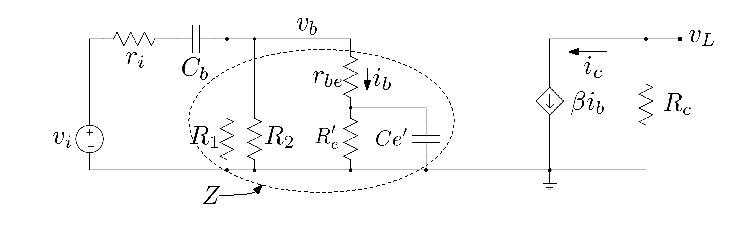
\includegraphics[scale=0.90]{commonEmitterCbCeLowCutoffFrequencyAEquivalent}
\caption{}
\label{شکل_تعددی_رد_عمل_قابو_مخارج_کپیسٹر_ب}
\end{figure}

دئے گئے قیمتیں پر کرتے ہیں۔
\begin{align*}
\frac{1}{Z}&=\frac{1}{40000}+\frac{1}{80000}+\frac{1}{200000}+4\times 10^{-6}\times s\\
&=\left(42.5+4s \right)\times 10^{-6}
%&=0.0000425+0.000004 s
\end{align*} 
مساوات \حوالہ{مساوات_تعددی_ردعمل_قابو_مخارج_کپیسٹر} میں کسر کے نیچے   سے \عددی{Z} باہر نکالتے ہوئے کسر کے اوپر موجود \عددی{Z} کے ساتھ کاٹتے ہوئے ملتا ہے
\begin{align*}
A_v=-R_c \beta \left(\frac{1}{R_e'}+s C_e' \right) \left(\frac{1}{\left(r_i+\frac{1}{sC_b}\right)\frac{1}{Z}+1} \right)
\end{align*}
اس میں قیمتیں پر کرتے ہیں
\begin{align*}
A_v&= \frac{-\left(1.96+1.568 s \right)}{\left(50000+\frac{1}{0.00004 s}\right)\left(42.5+4s \right)\times 10^{-6}+1}\\
&=\frac{-\left(1.96+1.568 s \right)}{2.125+0.2 s+\frac{1.0625}{s}+0.1+1}\\
&=\frac{-\left(1.96+1.568 s \right)}{3.225+0.2 s+\frac{1.0625}{s}}\\
&=\frac{-\left(1.96+1.568 s \right) s}{3.225 s+0.2 s^2+1.0625}\\
&=\frac{-\left(1.96+1.568 s \right) s}{0.2 s^2+3.225 s+1.0625}
\end{align*}
جسے یوں لکھا جا سکتا ہے
\begin{align*}
A_v&=\frac{-\left(1.96+1.568 s \right) s}{0.2 \left(s^2+16.125 s+5.3125\right)}\\
&=\frac{-6.25 \left(1.25+s \right) s}{\left(s+0.336 \right)\left(s+15.788 \right)}
\end{align*}
اس کو عمومی شکل میں لکھتے ہوئے اس کا بوڈا خط کھینچتے ہیں۔
\begin{align}\label{مساوات_تعددی_ردعمل_قابو_مخارج_عمومی_شکل_کی_مساوات}
A_v&=\frac{-1.8473\left(1+\frac{s}{1.25} \right) s}{\left(1+\frac{s}{0.336} \right)\left(1+\frac{s}{15.788}\right)}
\end{align}
%
\begin{figure}
\centering
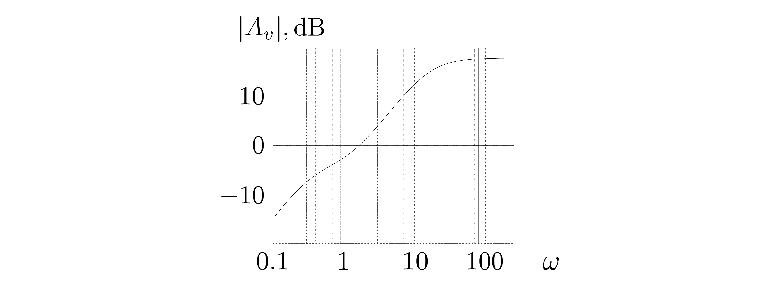
\includegraphics[scale=0.90]{bodeMagnitudeBaseAndEmitterCapacitorA}
\caption{}
\label{شکل_تعددی_ردعمل_سوال_قابو_مخارج_کپیسٹر_کونا}
\end{figure}
%
شکل \حوالہ{شکل_تعددی_ردعمل_سوال_قابو_مخارج_کپیسٹر_کونا} میں اس مساوات کا خط دکھایا گیا ہے۔

شکل \حوالہ{شکل_تعددی_رد_عمل_قابو_مخارج_کپیسٹر_ب} پر دوبارہ غور کریں۔\عددی{C_b} اور \عددی{C_e'} کے قیمتوں میں واضح فرق ہے۔کم تعدد پر \عددی{\tfrac{1}{\omega C_e'}} کی قیمت \عددی{\tfrac{1}{\omega C_b}} کے قیمت سے بہت زیادہ ہو گی۔یوں کم تعدد پر \عددی{C_e'} کو کھلے سرے تصور کرتے ہوئے \عددی{C_b} کے کردار پر غور کرتے ہیں۔\عددی{C_b} کے متوازی کل مزاحمت \عددی{R_{mCb}} مندرجہ ذیل ہے
\begin{align*}
R_{mCb}=r_i+ R_1 \mathbin{\|} R_2 \mathbin{\|} R_e'=\SI{73.529}{\kilo \ohm}
\end{align*}
یوں ہم توقع رکھتے ہیں کہ \عددی{C_b} سے
\begin{align*}
\frac{1}{R_{mCB} \times C_b}=\frac{1}{73.529 \times 10^3 \times 40 \times 10^{-6}}=\num{0.34}
\end{align*}
تعدد پر \اصطلاح{قطب} حاصل ہو گا۔ہم دیکھتے ہیں کہ یہ قطب مساوات \حوالہ{مساوات_تعددی_ردعمل_قابو_مخارج_عمومی_شکل_کی_مساوات} میں دئے \عددی{0.336} تعدد پر قطب کے تقریباً برابر ہے۔اسی طرح نہایت زیادہ تعدد پر \عددی{\tfrac{1}{\omega C_b}} کو قصر دور تصور کیا جا سکتا ہے۔ایسا کرتے ہوئے \عددی{C_e'} کے متوازی کل مزاحمت حاصل کرتے ہیں
\begin{align*}
\frac{1}{R_{mCe'}}=\frac{1}{r_i}+\frac{1}{R_1}+\frac{1}{R_2}+\frac{1}{R_e'}
\end{align*}
سے
\begin{align*}
R_{mCe'}=\SI{16}{\kilo \ohm}
\end{align*}
حاصل ہوتا ہے۔ہم توقع کرتے ہیں کہ یوں \عددی{C_e'} سے حاصل قطب
\begin{align*}
\frac{1}{R_{mCe'} \times C_e'}=\frac{1}{16 \times 10^{3} \times 4 \times 10^{-6}}=\SI{15.625}{\radian \per \second}
\end{align*}
پر پایا جائے گا۔ہم دیکھتے ہیں کہ یہ قطب مساوات \حوالہ{مساوات_تعددی_ردعمل_قابو_مخارج_عمومی_شکل_کی_مساوات} میں دئے \عددی{15.788} تعدد پر دئے قطب کے  تقریباً برابر ہے۔مساوات کا \اصطلاح{صفر}  \عددی{1.25} کے تعدد پر پایا جاتا ہے جو درحقیقت \عددی{\tfrac{1}{R_e C_e}} کے برابر ہے۔
%===========
\ابتدا{مثال}\شناخت{مثال_تعددی_ردعمل_قابو_مخارج_کپیسٹر_مشکل_حل}
مساوات \حوالہ{مساوات_تعددی_ردعمل_قابو_مخارج_کپیسٹر} کو حل کریں۔

حل: اس مساوات کو دوبارہ پیش کرتے ہیں۔
\begin{gather}
\begin{aligned} \label{مساوات_تعددی_ردعمل_قابو_مخارج_کپیسٹر_الف}
A_v =-R_c \beta \left(s C_e'+\frac{1}{R_e'} \right) \left[\frac{Z}{r_i+\frac{1}{sC_b}+Z} \right]
\end{aligned}
\end{gather}
جہاں \عددی{r_{be}} کو نظر انداز کرتے ہوئے
\begin{align*}
\frac{1}{Z}=\frac{1}{R_1}+\frac{1}{R_2}+\frac{1}{R_e'}+s C_e'=\frac{1}{R_m}+s C_e'
\end{align*}
کے برابر ہے جہاں
\begin{align*}
\frac{1}{R_m}=\frac{1}{R_1}+\frac{1}{R_2}+\frac{1}{R_e'}
\end{align*}
لیا گیا ہے۔مساوات \حوالہ{مساوات_تعددی_ردعمل_قابو_مخارج_کپیسٹر_الف} میں کسر کے نیچے   سے \عددی{Z} باہر نکالتے ہوئے کسر کے اوپر موجود \عددی{Z} کے ساتھ کاٹتے ہوئے ملتا ہے
\begin{align*}
A_v=-R_c \beta \left(s C_e'+\frac{1}{R_e'} \right) \left[\frac{1}{\left(r_i+\frac{1}{sC_b}\right)\frac{1}{Z}+1} \right]
\end{align*}
اس میں \عددی{Z} پُر کرتے ہوئے حل کرتے ہیں۔
\begin{align*}
A_v&=\frac{-R_c \beta \left(s C_e'+\frac{1}{R_e'} \right)}{\left(r_i+\frac{1}{sC_b}\right)\left(\frac{1}{R_m}+sC_e' \right)+1}\\
&=\frac{-R_c \beta \left(s C_e'+\frac{1}{R_e'} \right)}{\frac{r_i}{R_m}+s r_i C_e'+\frac{1}{s R_mC_b}+\frac{C_e'}{C_b}+1}
\end{align*}
کسر کے نچلے حصے میں \عددی{s} کی تعلق سے اجزاء اکٹھے کرتے  ہوئے حل کرتے ہیں۔
\begin{align*}
A_v&=\frac{-R_c \beta \left(s C_e'+\frac{1}{R_e'}\right)}{s r_i C_e'+\left(\frac{r_i}{R_m}+\frac{C_e'}{C_b}+1\right)+\frac{1}{s R_mC_b}}\\
&=\frac{-R_c \beta R_m C_b\left(s C_e'+\frac{1}{R_e'} \right) s}{s^2 r_i C_e' R_m C_b+s \left(\frac{r_i}{R_m}+\frac{C_e'}{C_b}+1\right) R_m C_b+1}\\
&=\frac{-R_c \beta R_m C_b  C_e' \left(s+\frac{1}{R_e'  C_e' }\right) s}{ r_i C_e' R_m C_b  \left[s^2+s \left(\frac{r_i}{R_m}+\frac{C_e'}{C_b}+1\right) \frac{1}{r_i C_e'}+\frac{1}{ r_i C_e' R_m C_b} \right]}
\end{align*}
اس مزید یوں لکھ سکتے ہیں۔
\begin{align*}
A_v&=\frac{\frac{-R_c \beta}{r_i}\left(s+\frac{1}{R_e'  C_e' }\right) s}{s^2+s \left(\frac{1}{R_m C_e'}+\frac{1}{r_i C_b}+\frac{1}{r_i C_e'}\right) +\frac{1}{ r_i C_e' R_m C_b}}\\
&=\frac{\frac{-R_c \beta}{r_i}\left(s+\frac{1}{R_e'  C_e' }\right) s}{s^2+s \left[\frac{1}{R_m C_e'}+\frac{1}{r_i} \left(\frac{1}{C_b}+\frac{1}{ C_e'} \right)\right] +\frac{1}{R_m C_e' r_i C_b}}
\end{align*}
اس مساوات میں
\begin{gather}
\begin{aligned}
\omega_c &=\frac{1}{R_e'  C_e' }=\frac{1}{R_e C_e}\\
\omega_1 &=\frac{1}{R_m C_e'}\\
\omega_2 &=\frac{1}{r_i} \left(\frac{1}{C_b}+\frac{1}{ C_e'} \right)\\
\omega_3 &=\frac{1}{r_i C_b}
\end{aligned}
\end{gather}
لکھتے ہوئے
\begin{align*}
A_v&=\frac{\frac{-R_c \beta}{r_i}\left(s+\omega_c\right) s}{s^2+s \left[\omega_1+\omega_2\right] +\omega_1 \omega_3}
\end{align*}
حاصل ہوتا ہے جسے یوں لکھا جا سکتا ہے
\begin{gather}
\begin{aligned}
A_v&=\frac{\frac{-R_c \beta}{r_i}\left(s+\omega_c\right) s}{\left(s+\omega_{q1} \right) \left(s+\omega_{q2} \right)}\\
&=\frac{\frac{-R_c \beta \omega_c}{\omega_{q1} \omega_{q2}} \left(\frac{s}{\omega_c}+1 \right) s}{\left(\frac{s}{\omega_{q1}}+1 \right)\left(\frac{s}{\omega_{q2}}+1 \right)}
\end{aligned}
\end{gather}
جہاں
\begin{gather}
\begin{aligned}
\omega_{q1}&= \frac{-\left(\omega_1+\omega_2 \right) - \sqrt{\left(\omega_1+\omega_2 \right)^2 -4 \omega_1 \omega_3}}{2}\\
\omega_{q2}&= \frac{-\left(\omega_1+\omega_2 \right) + \sqrt{\left(\omega_1+\omega_2 \right)^2 -4 \omega_1 \omega_3}}{2}
\end{aligned}
\end{gather}
ہیں۔
\انتہا{مثال}
%===========
\حصہ{بیس، ایمٹر اور کلکٹر  بیرونی کپیسٹروں کا مجموعی اثر}
مثال \حوالہ{مثال_تعددی_ردعمل_قابو_محاصل_کپیسٹر_دور_کونے} میں یہ حقیقت سامنے آئی کہ اگر کسی ایک کپیسٹر سے حاصل  کونا  کسی دوسرے کپیسٹر سے حاصل  کونے سے بہت بلند تعدد پر پایا جائے تب پست انقطاعی تعدد زیادہ تعدد پر پائے جانے والے کونے پر ہو گا۔ایمپلیفائر تخلیق دیتے ہوئے اس حقیقت کو عموماً بروئے کار لایا جاتا ہے۔

اسی طرح مثال \حوالہ{مثال_تعددی_ردعمل_قابو_مخارج_کپیسٹر_مشکل_حل} میں یہ حقیقت سامنے آئی کہ بیس  اور ایمٹر دونوں پر کپیسٹر نسب ہونے کی صورت میں دور کو حل کرنا دشوار ہوتا ہے اور اسے حل کرنے سے زیادہ قابل استعمال مساواتیں حاصل نہیں ہوتیں۔

عموماً ایمپلیفائر میں \عددیء{C_B}، \عددی{C_E} اور \عددی{C_C} تینوں پائے جاتے ہیں۔ایمپلیفائر کسی مخصوص اشارے کے لئے تخلیق دئے جاتا ہے۔اشارے کی کم سے کم اور زیادہ سے زیادہ ممکنہ تعدد کو مد نظر رکھتے ہوئے ایمپلیفائر تخلیق دیا جاتا ہے۔ایمپلیفائر کی پست انقطاعی تعدد اشارے کے کم سے کم ممکنہ تعدد سے کم رکھا جاتا ہے۔یوں ایمپلیفائر پست انقطاعی تعدد تک درمیانی تعدد کی افزائش برقرار رکھتا ہے جبکہ پست انقطاعی نقطے  سے کم تعدد پر ایمپلیفائر کی کارکردگی اہمیت نہیں رکھتی چونکہ اس خطے میں اسے استعمال نہیں کیا جاتا۔

\عددی{\omega_0=\frac{1}{R_m Cm}} لیتے ہوئے \عددی{C=\frac{1}{\omega_0 R_m}}  حاصل ہوتا ہے۔یوں کم \عددی{R_m} کی صورت میں \عددی{C} کی بڑی قیمت حاصل ہوتی ہے۔حقیقی ایمپلیفائر میں \عددی{C_E} کے ساتھ کل متوازی جڑی مزاحمت کی قیمت \عددی{C_B} اور \عددی{C_C} کے متوازی مزاحمتوں سے کم ہوتی ہے۔لہٰذا کسی بھی \عددی{\omega_0} کے لئے درکار \عددی{C_E} کی قیمت بقایا دو کپیسٹروں سے بڑی ہوتی ہے۔اسی لئے پست انقطاعی تعدد کو \عددی{C_E} کے مدد سے حاصل کیا جاتا ہے جبکہ \عددی{C_B} اور \عددی{C_C} سے حاصل انقطاعی نقطوں  کو اس سے کئی درجے کم تعدد پر رکھا جاتا ہے۔یوں حاصل \عددی{C_E} کی قیمت کم سے کم ہو گی۔اگر اس کے برعکس \عددی{C_B} یا \عددی{C_C} کی مدد سے درکار پست انقطاعی نقطہ حاصل کیا جائے تو اس صورت میں \عددی{C_E} سے حاصل نقطے  کو اس سے بھی کم تعدد پر رکھنا ہو گا جس سے \عددی{C_E} کی قیمت زیادہ حاصل ہو گی۔

آئیں ایک مثال کی مدد سے ایسے ایمپلیفائر  کا تجزیہ کریں۔

%==========
\ابتدا{مثال}\شناخت{مثال_تعددی_ردعمل_قباو_مخارج_محاصل_کپیسٹر_سادہ_حل}
شکل \حوالہ{شکل_تعددی_ردعمل_مثال_قابو_مخارج_اور_محاصل_کپیسٹر} میں \عددی{A_i=\tfrac{i_L}{i_i}} کا درمیانے تعدد پر افزائش \عددی{A_i=\tfrac{i_L}{i_i}} حاصل کریں۔اس کا پست انقطاعی تعدد بھی حاصل کریں۔

\begin{figure}
\centering
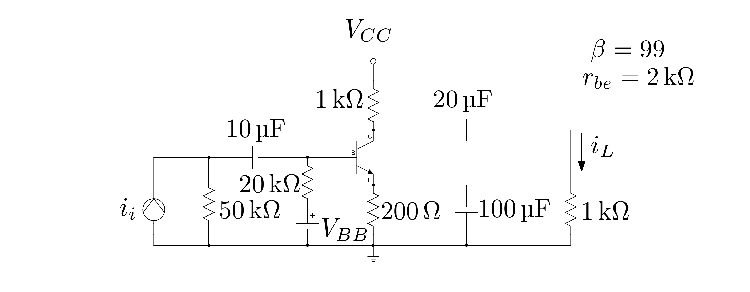
\includegraphics[scale=0.90]{exampleEmitterBaseAndCollectorCapacitors}
\caption{}
\label{شکل_تعددی_ردعمل_مثال_قابو_مخارج_اور_محاصل_کپیسٹر}
\end{figure}

حل:شکل \حوالہ{شکل_تعددی_ردعمل_سوال_قابو_مخارج_اور_محاصل_کپیسٹر_مساوی} میں مساوی دور دکھایا گیا ہے جہاں \عددی{R_e'=\left(\beta+1 \right) R_e} اور \عددی{C_e'=\tfrac{C_e}{\beta+1}} استعمال کئے گئے ہیں۔درمیانی تعدد پر تمام کپیسٹر قصر دور کردار ادا کریں گے۔یوں
\begin{align*}
A_i&=\frac{i_L}{i_c} \times \frac{i_c}{i_b} \times  \frac{i_b}{v_b} \times \frac{v_b}{i_i} \\
  &=\left(\frac{-1000}{2000}\right) \left( 99\right) \left( \frac{1}{2000}\right)\left(1754\right) \\
&=\SI[per=frac,fraction=nice]{-43}{\ampere \per \ampere}
\end{align*}
یعنی \عددی{\SI{32.67}{dB}} حاصل ہوتا ہے۔

ہم دیکھتے ہیں کہ \عددی{C_c} کی وجہ سے ایک عدد قطب
\begin{align*}
\omega_{qc}=\frac{1}{20 \times 10^{-6} \times 2000}=\SI[per=frac,fraction=nice]{25}{\radian \per \second}
\end{align*}
پر پایا جائے گا۔\عددی{C_e} اور \عددی{C_b} کے کردار پر اب غور کرتے ہیں۔\عددی{C_e} کا عکس ٹرانزسٹر کے بیس  جانب لیا گیا ہے جو کہ \عددی{\SI{1}{\micro \farad}} کے برابر ہے۔یوں جن تعدد پر \عددی{\SI{1}{\micro \farad}} اہمیت رکھتا ہے ان تعدد پر \عددی{C_b} بطور قصر دور کردار ادا کرے گا۔\عددی{C_b} کو قصر دور تصور کرتے ہوئے \عددی{\SI{1}{\micro \farad}} کے متوازی کل مزاحمت
\begin{align*}
R_e' \mathbin{\|} \left(r_{be}+r_i \mathbin{\|} R_b \right)=\SI{8.976}{\kilo \ohm}
\end{align*} 
حاصل ہوتا ہے  لہٰذا \عددی{\SI{1}{\micro \farad}} سے حاصل قطب
\begin{align*}
\omega_{qe}=\frac{1}{10^{-6} \times 8976}=\SI[per=frac,fraction=nice]{111.4}{\radian \per \second}
\end{align*}   
پر پایا جائے گا۔اسی طرح  جن تعدد پر \عددی{\SI{10}{\micro \farad}} اہمیت رکھتا ہے ان تعدد پر \عددی{\SI{1}{\micro \farad}} بطور کھلے دور کردار ادا کرے گا۔\عددی{\SI{1}{\micro \farad}} کو کھلے دور تصور کرتے ہوئے \عددی{\SI{10}{\micro \farad}} کے متوازی کل مزاحمت
\begin{align*}
r_i + R_b \mathbin{\|} \left[r_{be}+R_e' \right] =\SI{60.476}{\kilo \ohm}
\end{align*} 
حاصل ہوتا ہے اور یوں
\begin{align*}
\omega_{qb}=\frac{1}{10 \times 10^{-6} \times 60476}=\SI[per=frac,fraction=nice]{1.65}{\radian \per \second}
\end{align*}
پر قطب پایا جائے گا۔
%
\begin{figure}
\centering
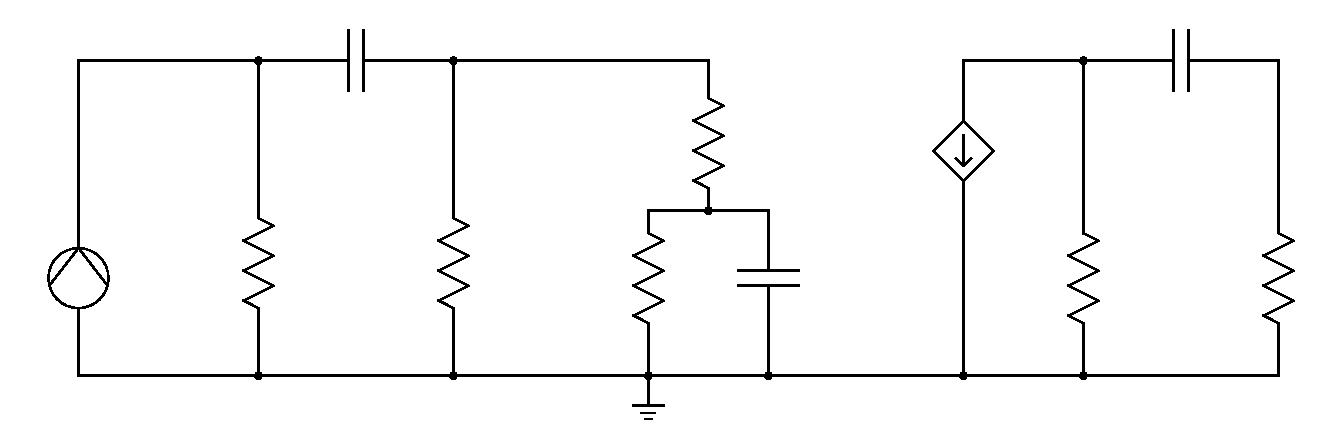
\includegraphics[scale=0.90]{emitterBaseAndCollectorCapacitorsEquivalent}
\caption{}
\label{شکل_تعددی_ردعمل_سوال_قابو_مخارج_اور_محاصل_کپیسٹر_مساوی}
\end{figure}
آپ نے دیکھا کہ
\begin{align*}
\omega_{qe} \gg \omega_{qc} \gg \omega_{qb}
\end{align*}
ہیں۔یوں پست انقطاعی تعدد \عددی{\omega_L=\omega_{qe}} پر پایا جائے گا۔

مندرجہ بالا حساب و کتاب میں \عددی{\omega_{qe}} پر ہم نے \عددی{C_b} کو قصر دور تصور کیا تھا جبکہ \عددی{\omega_{qb}} پر اسے کھلے دور تصور کیا تھا۔آئیں دیکھیں کہ کیا ایسا کرنا درست تھا۔\عددی{\omega_{qe}} پر \عددی{C_b} کی برقی رکاوٹ کی حتمی قیمت
\begin{align*}
\abs{\frac{1}{\omega_{qe} C_b}}&=\frac{1}{111.4 \times 10 \times 10^{-6}}=\SI{0.898}{\kilo \ohm}\\
\end{align*}
ہے۔\عددی{C_e'} کے متوازی کل مزاحمت کے لحاض سے یہ چھوٹی مقدار ہے جسے نظر انداز کیا جا سکتا ہے۔یوں آپ دیکھ سکتے ہیں کہ \عددی{\omega_{qe}} پر \عددی{C_b} کی برقی رکاوٹ کو نظر انداز کرتے ہوئے اسے قصر دور تصور کیا جا سکتا ہے۔اسی طرح \عددی{\omega_{qb}} پر
\begin{align*}
\abs{\frac{1}{\omega_{qb} C_e'}}&=\frac{1}{1.65 \times 10^{-6}}=\SI{606}{\kilo \ohm}
\end{align*}
ہے لہٰذا \عددی{\omega_{qb}} پر \عددی{C_e} کو کھلے دور تصور کیا جا سکتا ہے۔
\انتہا{مثال}
%==========
\حصہ{پست انقطاعی تعدد بذریعہ سورس کپیسٹر}
شکل \حوالہ{شکل_تعددی_ردعمل_مثال_ماسفیٹ_مخارج_کپیسٹر} میں گیٹ اور کلکٹر  کپیسٹروں کی قیمت لامحدود تصور کریں۔\عددی{A_v=\tfrac{v_L}{v_i}} حاصل کرتے ہوئے پست انقطاعی تعدد \عددی{\omega_L} حاصل کرتے ہیں۔
\begin{figure}
\centering
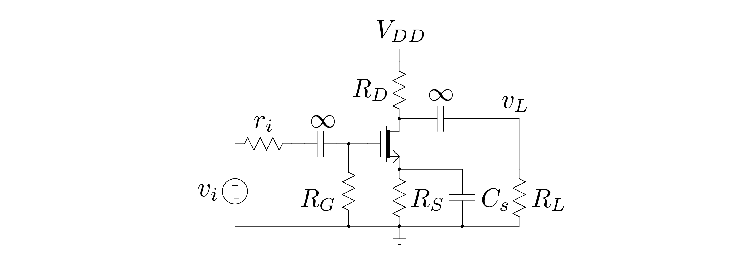
\includegraphics[scale=0.90]{nMosfetDepletionSourceCapacitorResponse}
\caption{}
\label{شکل_تعددی_ردعمل_مثال_ماسفیٹ_مخارج_کپیسٹر}
\end{figure}
گیٹ پر برقی دباو کو \عددی{v_i'} لکھتے ہیں جہاں
\begin{align*}
v_i'=\left(\frac{R_G}{r_i+R_G} \right) v_i
\end{align*}
کے برابر ہے۔یوں صفحہ \حوالہصفحہ{شکل_ماسفیٹ_مزاحمت_کے_عکس_ب} پر شکل \حوالہ{شکل_ماسفیٹ_مزاحمت_کے_عکس_ب} کے طرز پر موجودہ دور کا مساوی دور بناتے ہوئے شکل \حوالہ{شکل_تعددی_ردعمل_مثال_مخارج_کپیسٹر_مساوی} حاصل ہوتا ہے۔مساوی دور میں سورس پر پائے جانے والے برقی رکاوٹ
 \عددی{\left(\mu+1 \right)} سے ضرب ہو کر کلکٹر  منتقل ہوتے ہیں۔\عددی{C_s} کی رکاوٹ \عددی{\tfrac{1}{s C_s}} یوں
 \عددی{\tfrac{\mu+1}{s C_s}} ہو جائے گی یعنی کپیسٹر کی قیمت \عددی{\tfrac{C_s}{\mu+1}} ہو جائے گی۔
\begin{figure}
\centering
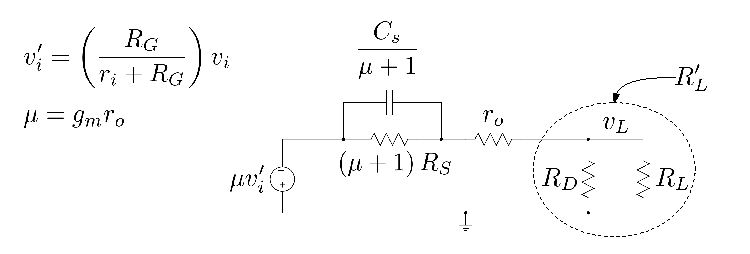
\includegraphics[scale=0.90]{nMosfetDepletionSourceCapacitorResponseEquivalent}
\caption{}
\label{شکل_تعددی_ردعمل_مثال_مخارج_کپیسٹر_مساوی}
\end{figure}

مساوی دور میں متوازی جڑے مزاحمت اور کپیسٹر کی کل برقی رکاوٹ کو \عددی{Z} لکھتے ہیں جہاں
\begin{align*}
\frac{1}{Z}&=\frac{1}{\left(\mu+1 \right)R_S}+\frac{s C_s}{\mu+1}\\
Z&=\frac{\left(\mu+1 \right)R_S}{1+s R_S C_s}
\end{align*}
کے برابر ہے۔اس طرح
\begin{align*}
v_L&=\left(\frac{R_L'}{Z +r_o +R_L'}\right) \left(-\mu v_i' \right)
\end{align*}
لکھا جا سکتا ہے جہاں \عددی{R_L'=\tfrac{R_L R_D}{R_L+R_D}} کے برابر ہے۔اس میں \عددی{Z} پُر کرتے ہیں۔
\begin{align*}
v_L&=\frac{-\mu R_L' v_i'}{\frac{\left(\mu+1 \right)R_S}{1+s R_S C_s} +r_o +R_L'}
\end{align*}
یوں
\begin{align*}
\frac{v_L}{v_i'}&=\frac{-\mu R_L' \left(1+s R_S C_s \right)}{\left(\mu+1 \right)R_S +\left(1+s R_S C_s \right)\left(r_o +R_L'\right)}\\
&=\frac{-\mu R_L' \left(1+s R_S C_s \right)}{\left(\mu+1 \right)R_S +r_o +R_L'+s R_S C_s \left(r_o +R_L'\right)}\\
&=\left(\frac{-\mu R_L'}{r_o+R_L'}\right)\frac{s+\frac{1}{ R_S C_s}}{s+\frac{\left(\mu+1 \right)R_S +r_o +R_L'}{R_S C_s \left(r_o +R_L'\right)}}
\end{align*}
حاصل ہوتا ہے۔پہلی قوسین  میں \عددی{\mu =g_m r_o} پر کرنے سے اس قوسین کو
\begin{align*}
\frac{-g_m r_o R_L'}{r_o+R_L'}&=-g_m \left(r_o\mathbin{\|} R_L' \right)\\
&=-g_m \left(r_o\mathbin{\|} R_L \mathbin{\|} R_D \right)\\
&= -g_m R_{\mathbin{\|}}
\end{align*}
لکھا جا سکتا ہے جہاں
\begin{align*}
R_{\mathbin{\|}}=r_o\mathbin{\|} R_L \mathbin{\|} R_D
\end{align*}
کے برابر ہے۔یوں
\begin{align*}
\frac{v_L}{v_i'}&=-g_m R_{\mathbin{\|}}\left[\frac{s+\frac{1}{ R_S C_s}}{s+\frac{\left(\mu+1 \right)R_S +r_o +R_L'}{R_S C_s \left(r_o +R_L'\right)}}\right]
\end{align*}
حاصل ہوتا ہے۔افزائش
\begin{align}\label{مساوات_تعدد_ردعمل_افزائش_ماسفیٹ_مخارج_کپیسٹر}
A_v =\frac{v_L}{v_i}&=\left(\frac{v_L}{v_i'}\right) \times \left(\frac{v_i'}{v_i}\right)\\
&=-g_m R_{\mathbin{\|}}\left[\frac{s+\frac{1}{ R_S C_s}}{s+\omega_L}\right] \left(\frac{R_G}{r_i+R_G} \right)
\end{align}
کے برابر ہے جہاں
\begin{align}\label{مساوات_تعددی_ردعمل_ماسفیٹ_مخارج_کپیسٹر}
\omega_L=\frac{\left(\mu+1 \right)R_S +r_o +R_L'}{R_S C_s \left(r_o +R_L'\right)}
\end{align}
پست انقطاعی تعدد ہے۔\عددی{\omega_L} کو مزید یوں لکھا جا سکتا ہے
\begin{align}
\omega_L=\frac{1}{R_m \frac{C_s}{\mu+1}}
\end{align}
جہاں \عددی{R_m} شکل \حوالہ{شکل_تعددی_ردعمل_مثال_مخارج_کپیسٹر_مساوی} میں \عددی{\tfrac{C_s}{\mu+1}} کے متوازی کل مزاحمت ہے یعنی
\begin{align*}
\frac{1}{R_m}&=\frac{1}{\left(\mu+1 \right) R_S}+\frac{1}{r_o+R_L'}\\
R_m&=\frac{\left(\mu+1 \right) R_S \left(r_o+R_L' \right)}{\left(\mu+1 \right)R_S+r_o+R_L'}
\end{align*}
درمیانی تعدد پر افزائش حاصل کرنے کی خاطر \عددی{\omega \to \infty} استعمال کرتے ہوئے مساوات  \حوالہ{مساوات_تعدد_ردعمل_افزائش_ماسفیٹ_مخارج_کپیسٹر} سے
\begin{align*}
A_{vD}=\eval{A_v}_{\omega \to \infty}&=-g_m R_{\mathbin{\|}}\left(\frac{R_G}{r_i+R_G} \right)\left[\frac{\infty+\frac{1}{ R_S C_s}}{\infty+\omega_L}\right] \\
&=-g_m R_{\mathbin{\|}}\left(\frac{R_G}{r_i+R_G} \right)
\end{align*}
حاصل ہوتا ہے۔عموماً \عددی{R_G \gg r_i} ہوتا ہے۔یوں
\begin{align}\label{مساوات_تعدد_ردعمل_درمیانی_تعدد_پر_افزائش_ماسفیٹ_مخارج_کپیسٹر}
A_{vD} \approx -g_m R_{\mathbin{\|}}
\end{align}
لکھا جا سکتا ہے۔
%===========
\ابتدا{مثال}\شناخت{مثال_تعددی_ردعمل_ماسفیٹ_مخارج_کپیسٹر}
شکل \حوالہ{شکل_تعددی_ردعمل_مثال_ماسفیٹ_مخارج_کپیسٹر} میں \عددیء{R_S=\SI{1}{\kilo \hertz}}، \عددیء{R_D=\SI{4.7}{\kilo \ohm}}، \عددی{R_L=\SI{100}{\kilo \ohm}}، \عددی{r_o=\SI{10}{\kilo \ohm}} اور \عددی{g_m=\SI{4}{\milli \siemens}} ہیں۔\عددی{f_L} کو \عددی{\SI{20}{\hertz}} پر رکھنے کی خاطر درکار \عددی{C_s} حاصل کریں۔درمیانی تعدد پر افزائش \عددی{A_v} بھی حاصل کریں۔

حل:مساوات \حوالہ{مساوات_تعددی_ردعمل_ماسفیٹ_مخارج_کپیسٹر} کی مدد سے
\begin{align*}
2 \times \pi \times 20=\frac{\left(0.004 \times 10000+1 \right)\times 1000 +10000 +4489}{1000\times C_s \left(10000 +4489\right)}
\end{align*}
یعنی \عددی{C_s=\SI{30.5}{\micro \farad}} حاصل ہوتا ہے۔مندرجہ بالا مساوات میں \عددی{R_L'=\SI{4489}{\ohm}} پُر کیا گیا ہے۔

مساوات \حوالہ{مساوات_تعدد_ردعمل_درمیانی_تعدد_پر_افزائش_ماسفیٹ_مخارج_کپیسٹر} میں
\begin{align*}
\frac{1}{R_{\mathbin{\|}}}&=\frac{1}{10000}+\frac{1}{100000}+\frac{1}{4700}=\num{3.22765e-4}\\
R_{\mathbin{\|}}&=\num{3098}
\end{align*}
پُر کرتے ہوئے
\begin{align*}
A_{vD}=-0.004 \times 3098=\SI{-12.4}{\volt \per \volt}
\end{align*}
حاصل ہوتا ہے۔
\انتہا{مثال}
%============


اب تک ہم نے جتنے بھی مثال دیکھے ان تمام میں بیرونی جڑے کپیسٹر کی وجہ سے پست انقطاعی نقطے  حاصل ہوئے۔آئیں اب ایک ایسا مثال دیکھیں جہاں بیرونی کپیسٹر کی وجہ سے زیادہ تعدد کا اشارہ متاثر ہوتا ہو۔اس مثال سے زیادہ تعدد کے مسائل بھی سامنے آئیں گے جن کا آگے تفصیلاً جائزہ لیا جائے گا۔

\ابتدا{مثال}\شناخت{مثال_تعددی_رد_عمل_بیرونی_کپیسٹر_بلند_انقطاعی_نقطہ}
شکل \حوالہ{شکل_تعددی_ردعمل_سوال_بار_کپیسٹر_الف} میں \عددی{A_v=\tfrac{v_L}{v_i}} کی مساوات حاصل کرتے ہوئے اس کا بوڈا خط کھینچیں۔
\begin{figure}
\centering
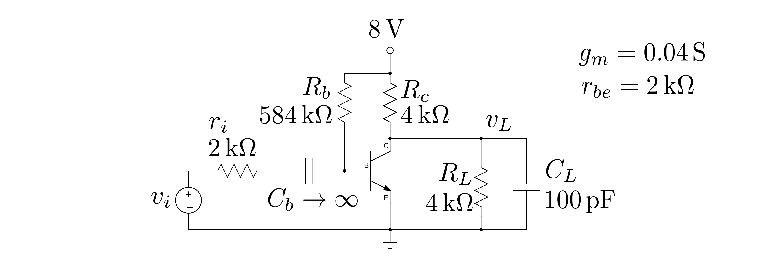
\includegraphics[scale=0.90]{questionFreqResponseLoadCapacitorA}
\caption{}
\label{شکل_تعددی_ردعمل_سوال_بار_کپیسٹر_الف}
\end{figure}

جل: اس کو آپ آسانی سے حل کر سکتے ہیں۔جواب مندرجہ ذیل ہے۔ 
\begin{align*}
A_v&= - g_m \left(\frac{R_b \mathbin{\|} r_{be}}{r_i+R_b \mathbin{\|} r_{be}} \right) \left(\frac{R_c \mathbin{\|} R_L  }{\frac{s}{\omega_q}+1}\right) = \frac{-40}{\frac{s}{\num{5e6}}+1}\\
\omega_q&=\tfrac{1}{\left(R_c \mathbin{\|} R_L \right) C_L}=\num{5e6}
\end{align*}
%
بوڈا خط شکل \حوالہ{شکل_تعددی_ردعمل_سوال_زمین_تک_کپیسٹر} میں دیا گیا ہے۔آپ دیکھ سکتے ہیں کہ \عددی{\omega_q} سے کم تعدد کے اشارات پر کپیسٹر کا کوئی اثر نہیں۔یوں \عددی{\omega_q} \اصطلاح{بلند انقطاعی تعدد}\فرہنگ{بلند انقطاعی تعدد} ہے۔
\begin{figure}
\centering
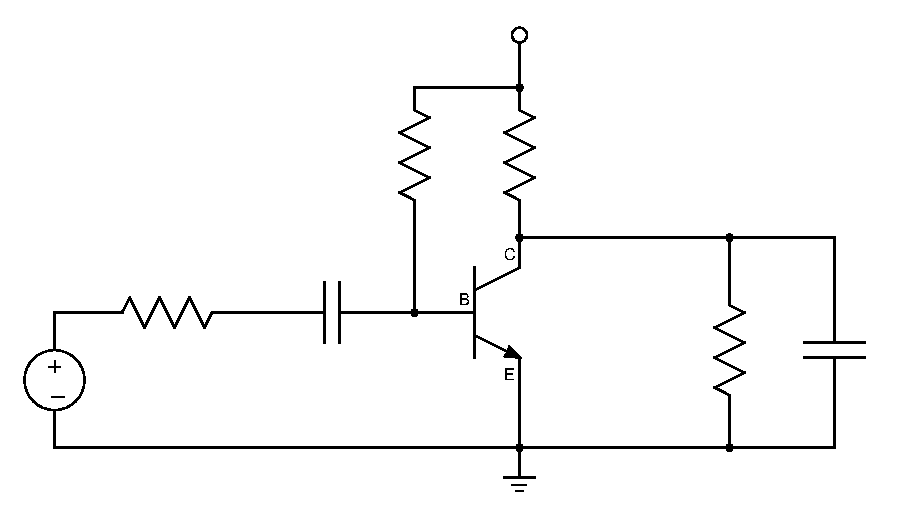
\includegraphics[scale=0.90]{bodeMagnitudeHighCutoffCollectorToGroundCapacitor}
\caption{}
\label{شکل_تعددی_ردعمل_سوال_زمین_تک_کپیسٹر}
\end{figure}
\انتہا{مثال}
%=========
\ابتدا{مثال}
مثال \حوالہ{مثال_تعددی_رد_عمل_بیرونی_کپیسٹر_بلند_انقطاعی_نقطہ} میں اگر داخلی اشارہ صفر وولٹ سے یکدم \عددی{\SI{20}{\milli \volt}} ہو جائے تو \عددی{v_L} نئی قیمت کے حتمی قیمت کے \عددی{\SI{90}{\percent}} کتنی دیر میں پہنچ پائے گا۔
\begin{figure}
\centering
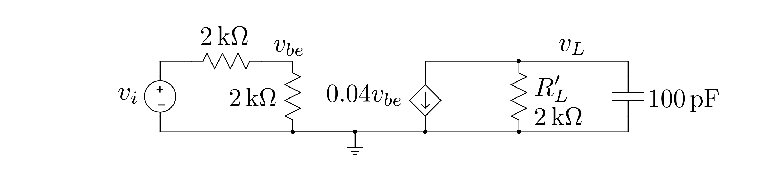
\includegraphics[scale=0.90]{bodeMagnitudeHighCutoffCollectorToGroundCapacitorEquivalent}
\caption{}
\label{شکل_تعددی_ردعمل_سوال_زمین_تک_کپیسٹر_مساوی_دور}
\end{figure}

حل:شکل \حوالہ{شکل_تعددی_ردعمل_سوال_زمین_تک_کپیسٹر_مساوی_دور} میں \عددی{R_b} کو نظر انداز اور \عددی{R_c \mathbin{\|} R_L} کو \عددی{R_L'} لکھتے ہوئے مساوی دور دکھایا گیا ہے۔جیسے ہی داخلی اشارہ  \عددی{\SI{20}{\milli \volt}} ہوتا ہے اسی دم \عددی{v_{be}=\SI{10}{\milli \volt}} ہو جائے گا اور یوں \عددی{i_c=\SI{0.4}{\milli \ampere}} ہو جائیں گے۔کرخوف کے قانون برائے برقی رو کے تحت خارجی جانب
\begin{align*}
C_L \frac{d v_L}{d t}+\frac{v_L}{R_L'} +g_m v_{be}=0\\
C_L \frac{d v_L}{d t}+\frac{v_L}{R_L'} +0.0004=0
\end{align*}
لکھا جا سکتا ہے جسے
\begin{align*}
\frac{d v_L}{d t}=-\frac{1}{R_L' C_L}\left(v_L +0.0004 R_L' \right)\\
\frac{d v_L}{d t}=-\frac{1}{R_L' C_L}\left(v_L +0.8 \right)
\end{align*}
یا
\begin{align*}
\frac{d v_L}{v_L +0.8}=-\frac{dt}{R_L' C_L}
\end{align*}
لکھتے ہیں۔اس کا تکمل لیتے ہیں
\begin{align*}
\int \frac{d v_L}{v_L +0.8}=-\frac{1}{R_L' C_L}\int  dt\\
\ln \left(v_L+0.8 \right)=-\frac{t}{R_L' C_L}+K'\\
v_L+0.8=K e^{-\frac{t}{R_L'C_L}}
\end{align*}
حاصل ہوتا ہے جہاں \عددی{K'} اور \عددی{K} تکمل کے مستقل ہیں۔\عددی{t=0} پر \عددی{v_L=0} سے \عددی{K=0.8} حاصل ہوتا ہے لہٰذا
\begin{align*}
v_L&=0.8 \left(e^{-\frac{t}{R_L'C_L}} -1\right)\\
&=0.8 \left(e^{-5\times 10^6 t} -1\right)
\end{align*}
لامحدود وقت گزرنے کے بعد یعنی \عددی{t \to \infty} پر  اس مساوات کے تحت \عددی{v_L=\SI{-0.8}{\volt}} ہو گا۔یوں اس قیمت کے \عددی{\SI{90}{\percent}} قیمت حاصل کرنے کی خاطر حل کرتے ہیں
\begin{align*}
-0.9 \times 0.8 &=0.8 \left(e^{-5\times 10^6 t} -1\right)\\
\end{align*}
جس سے \عددی{t=\SI{0.46}{\micro \second}} حاصل ہوتا ہے۔
\انتہا{مثال}
%================
اس مثال میں ہم نے دیکھا کہ داخلی اشارے کے تبدیلی کے کچھ دیر بعد خارجی اشارہ اپنی نئی قیمت تک پہنچ پاتا ہے۔آپ دیکھ سکتے ہیں کہ تیز رفتار عددی ادوار میں \عددی{C_L} کی قیمت کم سے کم رکھنا نہایت ضروری ہے۔جہاں بھی تیز رفتار سے تبدیل ہونے والا اشارہ پایا جائے وہاں  \عددی{C_L} در حقیقت غیر ضروری نا پسندیدہ کپیسٹر ہوتا ہے جسے کم کرنے کی پوری کوشش کی جاتی ہے۔اس مثال میں کپیسٹر کی بدولت دور کے رفتار میں سستی پیدا ہونا دیکھا گیا۔آئیں اب بلند تعدد انقطاعی نقطوں پر غور کریں اور جن کپیسٹروں سے یہ نقطے پیدا ہوتے ہیں ان کی نشاندہی کریں۔پہلے \اصطلاح{مسئلہ ملر} پر غور کرتے ہیں جو آگے بار بار استعمال ہو گا۔
%================

\حصہ{مسئلہ ملر}
ٹرانزسٹر ایمپلیفائر کا بلند تعددی رد عمل دیکھنے سے پہلے شکل \حوالہ{شکل_تعددی_ردعمل_مسئلہ_ملر} کی مدد سے \اصطلاح{مسئلہ ملر}\فرہنگ{مسئلہ مل}\فرہنگ{Miller theorem}\حاشیہب{Miller theorem'} پر غور کرتے ہیں\حاشیہد{جان ملٹن ملر نے اس مسئلے کو دریافت کیا}۔
\begin{figure}
\centering
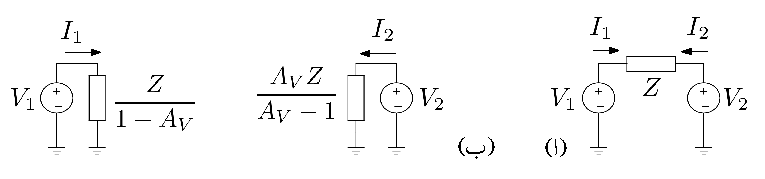
\includegraphics[scale=0.90]{millerEffect}
\caption{مسئلہ ملر}
\label{شکل_تعددی_ردعمل_مسئلہ_ملر}
\end{figure}
شکل  الف میں دو برقی دباو کے مابین برقی رکاوٹ \عددی{Z} نسب کی گئی ہے۔\عددی{V_1} سے باہر نکلتے برقی رو کو \عددی{I_1} سے ظاہر کرتے ہوئے
\begin{align*}
I_1=\frac{V_1-V_2}{Z}
\end{align*}
حاصل ہوتا ہے۔آئیں اس برقی رو کو قدر مختلف طریقے سے لکھیں۔
\begin{align*}
I_1 &=\frac{V_1-V_2}{Z}\\
&=V_1 \left(\frac{1-\frac{V_2}{V_1}}{Z} \right)\\
&=\frac{V_1}{\left(\frac{Z}{1-\frac{V_2}{V_1}} \right)}
\end{align*}
جس کو مزید یوں لکھ سکتے ہیں۔
\begin{align}
I_1 &=\frac{V_1}{Z_M}
\end{align}
جہاں
\begin{align}
Z_M=\frac{Z}{1-\frac{V_2}{V_1}}
\end{align}
کے برابر ہے۔اس مساوات میں
\begin{align}
\frac{V_2}{V_1}=A_V
\end{align}
لکھتے ہوئے
\begin{align} \label{مساوات_تعدد_ردعمل_ملر_رکاوٹ}
Z_M=\frac{Z}{1-A_V}
\end{align}
حاصل ہوتا ہے۔

شکل \حوالہ{شکل_تعددی_ردعمل_مسئلہ_ملر} ب میں \عددی{V_1} کے ساتھ \عددی{Z_M} جوڑا دکھایا گیا ہے۔جہاں تک \عددی{V_1} کا تعلق ہے، شکل  الف اور شکل  ب دونوں میں \عددی{V_1} سے بالکل یکساں \عددی{ِI_1} برقی رو حاصل ہوتا ہے۔یوں \عددی{V_1} کے نقطہ نظر سے شکل  الف کے طرز پر لگائے گئے \عددی{Z} اور شکل  ب کے طرز پر لگائے گئے \عددی{Z_M}  مساوی ادوار ہیں۔\عددی{Z_M} \اصطلاح{ملر} برقی رکاوٹ پکارا جاتا ہے۔\حاشیہد{\عددی{Z_M} لکھتے ہوئے زیر نوشت میں بڑے حروف تہجی میں \عددی{M} ملر کو ظاہر کرتا ہے}

آئیں اب \عددی{V_2} کے نقطہ نظر سے دیکھیں جس سے باہر نکلتے ہوئے برقی رو کو \عددی{I_2} سے ظاہر کرتے ملتا ہے
\begin{align*}
I_2&=\frac{V_2 - V_1}{Z}\\
&=V_2 \left(\frac{1-\frac{V_1}{V_2} }{Z}\right)\\
&=\frac{V_2}{\left(\frac{Z}{1-\frac{V_1}{V_2}} \right)}
\end{align*}
جسے
\begin{align}
I=\frac{V_2}{Z_M'}
\end{align}
لکھ سکتے ہیں جہاں
\begin{align*}
Z_M'&=\frac{Z}{1-\frac{V_1}{V_2}}\\
&=\frac{Z}{\frac{V_1}{V_2}  \left(\frac{V_2}{V_1}-1 \right)}\\
&=\frac{\left(\frac{V_2}{V_1} \right) Z}{\frac{V_2}{V_1} -1}
\end{align*}
یعنی
\begin{align} \label{مساوات_تعدد_ردعمل_ملر_رکاوٹ_الف}
Z_M'=\frac{A_V Z}{A_V-1}
\end{align}
کے برابر ہے۔شکل \حوالہ{شکل_تعددی_ردعمل_مسئلہ_ملر} میں \عددی{V_2} کے ساتھ \عددی{Z} کی جگہ \عددی{Z_M'} جوڑا دکھایا گیا ہے۔\عددی{V_2} کے نقطہ نظر سے شکل  الف اور شکل  ب مساوی ادوار ہیں۔ 
\begin{figure}
\centering
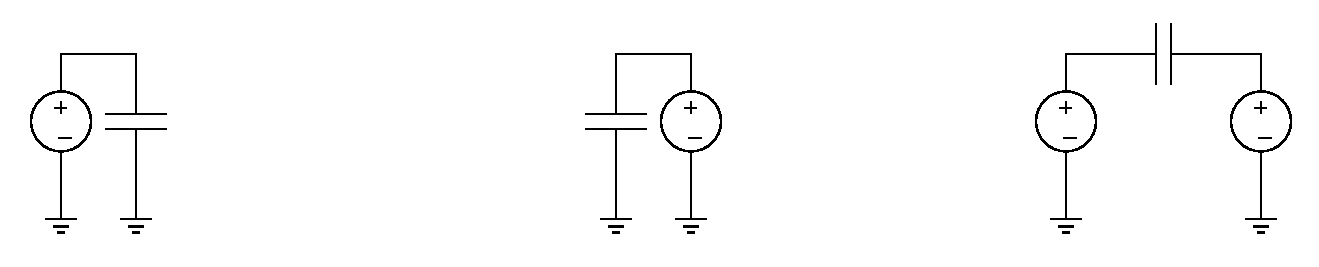
\includegraphics[scale=0.90]{millerCapacitors}
\caption{ملر کپیسٹر}
\label{شکل_تعددی_ردعمل_ملر_کپیسٹر}
\end{figure}

شکل \حوالہ{شکل_تعددی_ردعمل_مسئلہ_ملر} میں \عددی{Z} کی جگہ کپیسٹر \عددی{C} نسب کرنے سے شکل \حوالہ{شکل_تعددی_ردعمل_ملر_کپیسٹر} حاصل ہوتا ہے۔مساوات \حوالہ{مساوات_تعدد_ردعمل_ملر_رکاوٹ} میں کپیسٹر کی برقی رکاوٹ کو \عددی{\frac{1}{j \omega C}} لکھتے ہوئے
\begin{align*}
\frac{1}{j \omega C_M}&= \frac{\left(\frac{1}{j \omega C} \right)}{1-A_V}\\
&=\frac{1}{j \omega C \left(1-A_V \right)}
\end{align*}
یعنی
\begin{align} \label{مساوات_تعددی_ردعمل_ملر_کپیسٹر}
C_M=C \left(1-A_V \right)
\end{align}
حاصل ہوتا۔اسی طرح مساوات \حوالہ{مساوات_تعدد_ردعمل_ملر_رکاوٹ_الف} سے 
\begin{align*}
\frac{1}{j \omega C_M'}&=\frac{A_V \left(\frac{1}{j \omega C} \right)}{A_V -1} \\
&=\frac{A_V}{j \omega C \left(A_V -1 \right)}\\
&=\frac{1}{j \omega C \left(1-\frac{1}{A_V} \right)}
\end{align*}
یعنی
\begin{align} \label{مساوات_تعددی_ردعمل_ملر_کپیسٹر_الف}
C_M'=C \left(1-\frac{1}{A_V} \right)
\end{align}
حاصل ہوتا۔مساوات \حوالہ{مساوات_تعددی_ردعمل_ملر_کپیسٹر} کا اگلے حصے میں بار بار استعمال ہو گا۔\عددی{C_M} \اصطلاح{ملر کپیسٹر}\فرہنگ{ملر کپیسٹر}\فرہنگ{Miller's capacitor}\حاشیہب{Miller's capacitor} پکارا جاتا ہے۔

\حصہ{بلند تعددی رد عمل}
گزشتہ حصوں میں پست تعدد پر ٹرانزسٹر ایمپلیفائر کی کارکردگی دیکھی گئی جہاں ٹرانزسٹر کے ساتھ بیرونی جڑے کپیسٹروں کی وجہ سے پائے جانے والے پست انقطاعی نقطوں پر غور کیا گیا۔اس حصے میں بلند تعدد پر ایمپلیفائر کی کارکردگی دیکھی جائے گی۔بلند تعدد پر ٹرانزسٹر کے ساتھ بیرونی جڑے کپیسٹروں کی برقی رکاوٹ  \عددی{\frac{1}{\omega C}} نہایت کم ہوتی ہے اور یوں انہیں قصر دور تصور کیا جاتا ہے۔بلند تعدد پر ٹرانزسٹر کے اندرونی کپیسٹروں کی وجہ سے بلند انقطاعی نقطہ  پیدا ہوتا ہے جس پر اس حصے میں غور کیا جائے گا۔پہلے \عددی{npn} ٹرانزسٹر کو مثال بناتے ہوئے ان اندرونی کپیسٹروں پر تبصرہ کرتے ہیں۔

\جزوحصہ{بلند تعددی پائے \عددی{\pi} ریاضی نمونہ }\شناخت{حصہ_تعددی_ردعمل_بلند_تعددی_پائے_ماڈل}
استعمال کے دوران ٹرانزسٹر کےبیس-ایمٹر    جوڑ  کو الٹ مائل رکھا جاتا ہے۔بالکل ڈایوڈ کی طرح،اس  الٹ مائل \عددی{pn} جوڑ پر ویران خطہ پایا جاتا ہے جس کے ایک جانب مثبت بار جبکہ دوسری جانب منفی بار پایا جاتا ہے۔یہ دو الٹ قسم کے بار مل کر کپیسٹر کو جنم دیتے ہیں جسے \عددی{C_{b'c}} کی علامت سے پہچانا جاتا ہے۔اس کپیسٹر کی قیمت نہایت کم ہوتی ہے جو پست تعدد پر چلنے والے ٹرانزسٹروں میں \عددی{\SI{30}{\pico \farad}} کے لگ بھگ  جبکہ بلند تعدد پر چلنے والے ٹرانزسٹروں میں \عددی{\SI{1}{\pico \farad}} یا اس سے بھی کم ہوتی ہے۔اس کپیسٹر کی قیمت الٹا مائل کرنے والے برقی دباو \عددی{V_{CB}} پر منحصر ہوتی ہے.حقیقت میں \عددی{C_{b'c}} کی قیمت \عددی{V_{CB}^{-\frac{1}{2}}} یا  \عددی{V_{CB}^{-\frac{1}{3}}} کے تناسب  سے تبدیل ہوتی ہے۔صنعت کار عموماً \عددی{C_{b'c}} کو \عددی{C_{ob}} پکار کر اس کی قیمت کپیسٹر کے معلوماتی صفحات میں پیش کرتا ہے۔

اس کے علاوہبیس-ایمٹر    جوڑ پر  کپیسٹر \عددی{C_{b'e}} پایا جاتا ہے جس کی قیمت \عددی{\SI{100}{\pico \farad}} تا \عددی{\SI{5000}{\pico \farad}} پائی جاتی ہے۔آئیں دیکھیں کہ یہ کپیسٹر کس طرح پیدا ہوتا ہے۔ٹرانزسٹر کےبیس-ایمٹر    جوڑ پر  مثبت اشارے  کی موجودگی میں ایمٹر    سے بیس  کی جانب آزاد الیکٹران رواں ہوتے ہیں جن کا بیشتر حصہ بیس  خطے سے بذریعہ نفوذ گزر کر آخر کار کلکٹر  پہنچ  کر \عددی{i_c} کا حصہ بنتے ہیں۔اب تصور کریں کہ اس سے پہلے کہ الیکٹران بیس  خطے سے گزر پائیں، مہیا کردہ اشارہ  منفی ہو جاتا ہے۔آزاد الیکٹران اشارے کی نئی حقیقت کو دیکھتے ہوئے واپس ایمٹر     سرے کی جانب چل پڑیں گے۔نتیجتاً کلکٹر  سرے پر برقی رو \عددی{i_c} کی مقدار نسبتاً کم ہو جائے گی۔اس عمل کو مد نظر رکھتے ہوئے آپ دیکھ سکتے ہیں کہ ٹرانزسٹر کے کارکردگی کے لئے ضروری ہے کہ بیس  خطے سے الیکٹران کے گزرنے کا دورانیہ مہیا کردہ اشارے  کے دوری عرصے سے کم ہو۔جیسے جیسے اشارے کی تعدد بڑھائی جائے، ویسے ویسے کلکٹر  برقی رو \عددی{i_c} کی قیمت کم ہوتی جاتی ہے۔بڑھتی تعدد کی وجہ سے کم برقی رو کے حصول کو کپیسٹر \عددی{C_{b'e}} سے ظاہر کیا جاتا ہے۔بدلتے اشارے کی وجہ سے بیس  خطے سے گزرنے والے آزاد الیکٹران کبھی کلکٹر  اور کبھی ایمٹر    کی جانب پہنچنے کی کوشش ہی کرتے رہ جاتے ہیں۔یوں بیس  خطے میں گھیرے الیکٹرانوں کی تعداد کل برقی رو \عددی{I_{EQ}} پر منحصر ہوتی ہے۔\عددی{C_{b'e}} کی مقدار بیس  خطے میں گھیرے بار کی مقدار پر منحصر ہوتی ہے اور یوں اس کی قیمت برقی رو کے راست تناسب ہوتی ہے۔ٹرانزسٹر کے اندرونی کپیسٹروں کو شکل \حوالہ{شکل_تعددی_ردعمل_اندرونی_کپیسٹر} میں بطور بیرونی کپیسٹر دکھایا گیا ہے۔
\begin{figure}
\centering

\includegraphics[scale=0.90]{transistorCapacitors}
\caption{ٹرانزسٹر کے اندرونی کپیسٹر کو بطور بیرونی کپیسٹر دکھایا گیا ہے}
\label{شکل_تعددی_ردعمل_اندرونی_کپیسٹر}
\end{figure}
%
\begin{figure}
\centering
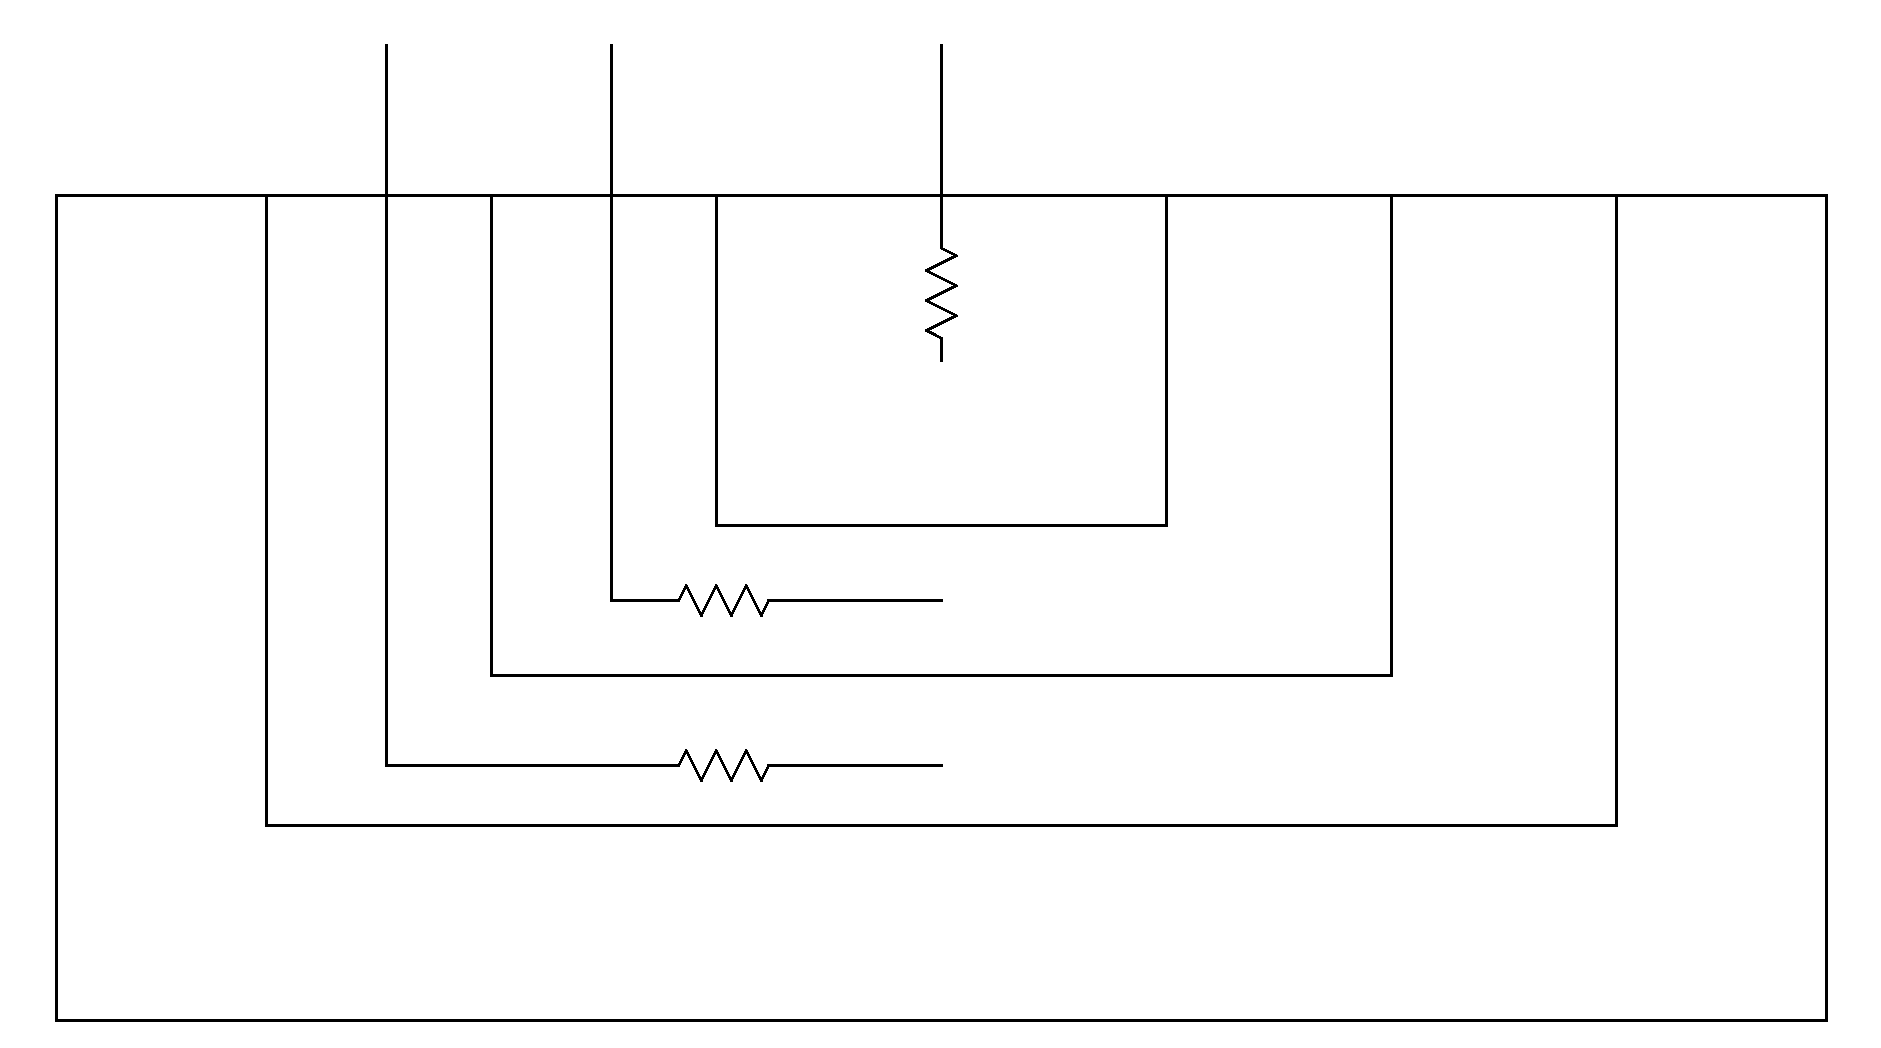
\includegraphics[scale=0.90]{transistorInternalResistors}
\caption{ٹرانزسٹر کے اندرونی مزاحمت}
\label{شکل_تعددی_ردعمل_اندرونی_مزاحمت}
\end{figure}

شکل \حوالہ{شکل_تعددی_ردعمل_اندرونی_مزاحمت} میں ٹرانزسٹر کی ساخت دکھائی گئی ہے جہاں بیرونی سروں کو حسب معمول \عددی{E}، \عددی{B} اور \عددی{C} کہا گیا ہے۔ٹرانزسٹر کے بیس  کے بیرونی سرے \عددی{B} اور اندرونی نقطہ \عددی{B'} کے درمیان \اصطلاح{غیر مطلوب مزاحمت}\فرہنگ{غیر مطلوب مزاحمت}\حاشیہب{parasitic resistor}\فرہنگ{parasitic resistor} \عددی{r_{bb'}} پایا جاتا ہے۔یہ مزاحمت بیس  خطے کی خصوصیات پر منحصر ہوتا ہے۔اسی طرح ایمٹر    پر \عددی{r_{ee'}} اور کلکٹر  پر \عددی{r_{cc'}} غیر مطلوب مزاحمت پائے جاتے ہیں۔الٹ مائلبیس-ایمٹر    جوڑ میں الٹی جانب یک سمتی  برقی رو کو مزاحمت \عددی{r_{\mu}} سے ظاہر کیا جاتا ہے۔اس کتاب میں \عددیء{r_{cc'}}،\عددیء{r_{ee'}} اور \عددی{r_{\mu}} کو صفر تصور کرتے ہوئے نظر انداز کیا جائے گا۔  
\begin{figure}
\centering
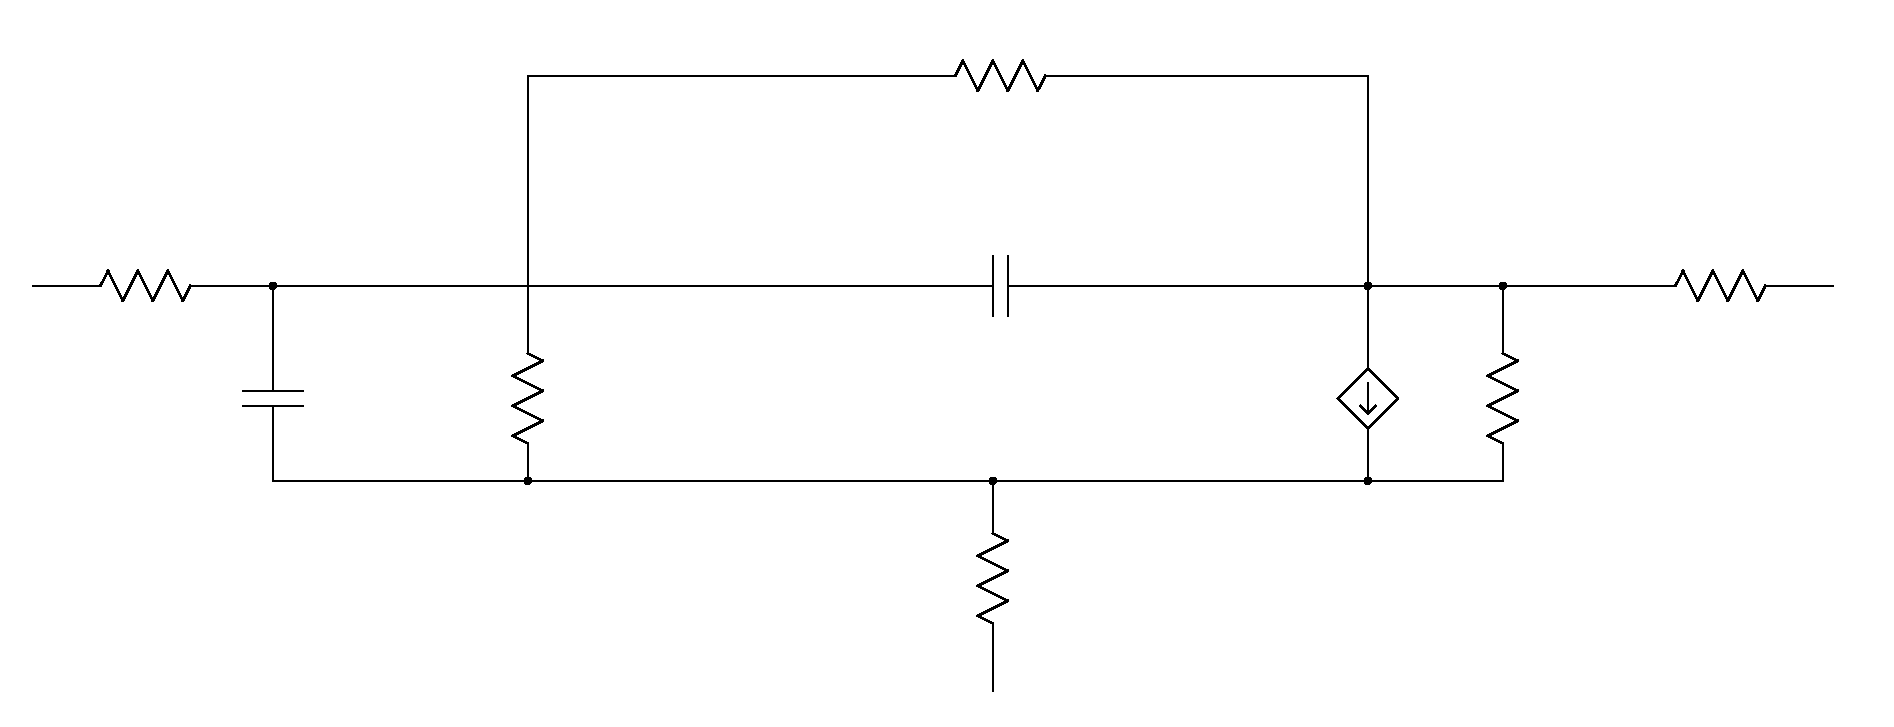
\includegraphics[scale=0.90]{transistorHighFreqPiModelA}
\caption{بلند تعددی پائے ریاضی نمونہ }
\label{شکل_تعددی_ردعمل_بلند_تعددی_ماڈل_الف}
\end{figure}

ٹرانزسٹر کے پست تعددی پائے ریاضی نمونے میں ان تمام اجزاء کی شمولیت سے بلند تعددی پائے ریاضی نمونہ حاصل ہوتا ہے جس کو شکل \حوالہ{شکل_تعددی_ردعمل_بلند_تعددی_ماڈل_الف} میں دکھایا گیا ہے۔شکل \حوالہ{شکل_تعددی_ردعمل_بلند_تعددی_ماڈل} الف میں اسی کا سادہ دور دکھایا گیا ہے  جس میں \عددیء{r_{cc'}}،\عددیء{r_{ee'}} اور \عددی{r_{\mu}} کو نظر انداز کیا گیا ہے۔اس ریاضی نمونے کو قلم و کاغذ سے حل کرنا زیادہ آسان ثابت ہوتا ہے۔اس کتاب میں اسی ریاضی نمونے کو استعمال کیا جائے گا۔

\عددی{r{bb'}} کی قیمت بیس  خطے کی چوڑائی کے راست تناسب ہوتی ہے۔پست تعددی ٹرانزسٹر کے بیس  خطے کی چوڑائی بلند تعددی ٹرانزسٹر کے بیس  خطے کی چوڑائی سے زیادہ ہوتی ہے۔اسی لئے پست تعددی ٹرانزسٹر کی \عددی{r_{bb'}} بلند تعددی ٹرانزسٹر کے \عددی{r{bb'}} سے زیادہ ہوتی ہے۔\عددی{r_{bb'}} کو مستقل تصور کیا جاتا ہے جس کی قیمت \عددی{\SI{10}{\ohm}} تا \عددی{\SI{50}{\ohm}} ہوتی ہے۔پست تعددی پائے ریاضی نمونے کے جزو \عددی{r_{be}} کو یہاں \عددی{r_{b'e}} کہا گیا ہے۔یوں مساوات \حوالہ{مساوات_ٹرانزسٹر_داخلی_مزاحمت_بالمقابل_رو} کے تحت
\begin{align}
r_{b'e}=\frac{\beta V_T}{I_{CQ}}
\end{align}
کے برابر ہے۔\عددی{v_{b'e}=i_b' r_{b'e}} لکھتے ہوئے اور مساوات \حوالہ{مساوات_ٹرانزسٹر_داخلی_مزاحمت_بالمقابل_موصلیت_نما} سے \عددی{g_m=\frac{\beta}{r_{b'e}}} کے استعمال سے شکل  الف کے \عددی{i_c=g_m v_{b'e}} کو \عددی{i_c=\beta i_b'} لکھا کا سکتا ہے جس سے قدرِ مختلف شکل  ب میں دکھایا گیا بلند تعددی پائے ریاضی نمونہ  حاصل ہوتا ہے۔شکل  ب میں \عددی{i_b'} پر دوبارہ غور کریں۔یہ \عددی{r_{b'e}} میں سے گزرتی برقی رو ہے نا کہ ٹرانزسٹر کے بیرونی بیس  سرے پر پائی جانے والی برقی رو۔ٹرانزسٹر اس برقی رو کے نسبت سے \عددی{i_c} خارج کرتا ہے۔بلند تعدد پر \عددی{c_{b'e}} کے راستے داخلی برقی رو کا کچھ حصہ گزرے گا جس کی وجہ سے ٹرانزسٹر کی افزائش میں کمی رونما ہو گی۔
\begin{figure}
\centering
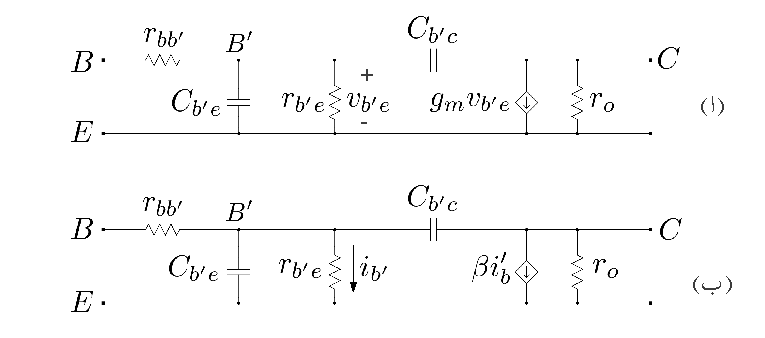
\includegraphics[scale=0.90]{transistorHighFreqPiModel}
\caption{سادہ بلند تعددی پائے ریاضی نمونہ }
\label{شکل_تعددی_ردعمل_بلند_تعددی_ماڈل}
\end{figure}
ٹرانزسٹر کے پست تعددی ٹی ریاضی نمونے کو صفحہ \حوالہصفحہ{شکل_ٹی_ماڈل} پر شکل \حوالہ{شکل_ٹی_ماڈل} میں دکھایا گیا ہے۔شکل \حوالہ{شکل_ٹی_ماڈل} پ میں ٹرانزسٹر کے اندرونی کپیسٹر کے شمولیت سے شکل \حوالہ{شکل_تعددی_ردعمل_بلند_تعددی_ٹی_ماڈل} حاصل ہوتا ہے جس میں \عددی{r_{bb'}} شامل نہیں کیا گیا۔ٹی ریاضی نمونے کا استعمال مشترکہ بیس  ایمپلیفائر حل کرتے وقت آتا ہے جہاں \عددی{r_{bb'}} کے اثر کو نظرانداز کرنا ممکن ہوتا ہے۔ٹی ریاضی نمونے میں \عددی{i_e} وہ برقی رو ہے جو اندرونی مزاحمت \عددی{r_e} میں سے گزرتی ہے۔
\begin{figure}
\centering
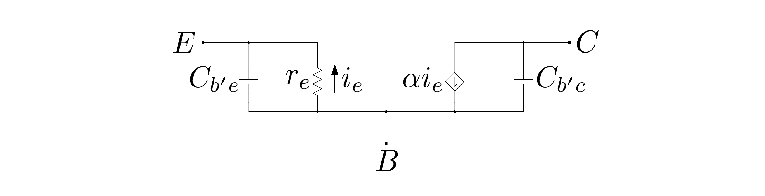
\includegraphics[scale=0.90]{highFreqTmodel}
\caption{بلند تعددی ٹی ریاضی نمونہ }
\label{شکل_تعددی_ردعمل_بلند_تعددی_ٹی_ماڈل}
\end{figure}

\جزوحصہ{مشترکہ ایمٹر بلند انقطاعی تعدد}
شکل \حوالہ{شکل_تعددی_ردعمل_بلند_تعددی_ماڈل} الف کے خارجی جانب برقی بوجھ \عددی{R_L} جوڑ کر افزائش برقی رو \عددی{A_i=\frac{i_L}{i_i}} حاصل کی جا سکتی ہے جس کی قیمت \عددی{R_L} بڑھانے سے گھٹے گی۔ایسا کرنے کی بجائے، جیسا کہ شکل \حوالہ{شکل_تعددی_ردعمل_کسر_دور_افزائش} الف میں دکھایا گیا ہے، ہم \عددی{R_L=0} رکھتے ہوئے قصر دور افزائش برقی رو \عددی{A_i} حاصل کرتے ہیں جو اس کی زیادہ سے زیادہ ممکنہ قیمت ہے۔چونکہ \عددی{R_L=0} سے مراد ٹرانزسٹر کے  کلکٹر  کو اس کے ایمٹر    کے ساتھ جوڑنا ہے لہٰذا ایسا کرنے سے \عددی{r_o} بھی قصر دور ہو جاتا ہے اور ساتھ ہی ساتھ \عددی{C_{b'c}} کا ایک سرا  برقی زمین کے ساتھ جڑ جاتا ہے۔چانکہ ٹرانزسٹر کا ایمٹر    بھی برقی زمین پر ہے لہٰذا \عددی{C_{b'c}} کا یہ سرا ایمٹر    کے ساتھ جڑ جاتا ہے۔ان حقائق کو مد نظر رکھتے ہوئے شکل  ب حاصل ہوتا ہے۔شکل  الف میں ہم دیکھتے ہیں کہ \عددی{C_{b'c}} میں داخلی جانب سے خارجی جانب برقی رو گزرے گی جبکہ شکل  ب میں ایسا نہیں ہوتا۔ہم \عددی{C_{b'c}} میں داخلی جانب سے خارجی جانب گزرتے ہوئے برقی رو کو نظر انداز کرتے ہوئے شکل \حوالہ{شکل_تعددی_ردعمل_کسر_دور_افزائش} کی مدد سے  \عددی{A_i} کی زیادہ سے زیادہ ممکنہ قیمت حاصل کرتے ہیں۔شکل میں
\begin{figure}
\centering
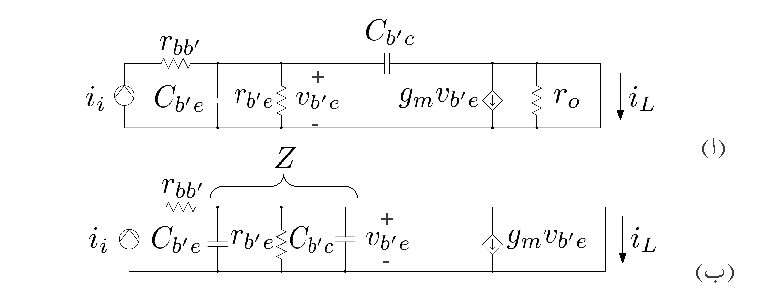
\includegraphics[scale=0.90]{transistorShortCircuitGain}
\caption{قصر دور برقی رو افزائش}
\label{شکل_تعددی_ردعمل_کسر_دور_افزائش}
\end{figure}
%
\begin{align*}
\frac{1}{Z}&=sC_{b'e}+s C_{b'c}+\frac{1}{r_{b'e}}\\
&=\frac{s\left(C_{b'e}+C_{b'c} \right ) r_{b'e}+1}{r_{b'e}}
\end{align*}
سے
\begin{align*}
Z=\frac{r_{b'e}}{s\left(C_{b'e}+C_{b'c} \right ) r_{b'e}+1}
\end{align*}
حاصل ہوتا ہے۔یوں
\begin{align*}
\eval {A_i}_{v_{ce}=0}&=\frac{i_L}{i_i}=\left(\frac{i_L}{i_c}\right) \left(\frac{i_c}{v_{b'e}}\right) \left(\frac{v_{b'e}}{i_i}\right)\\
&=\left(-1 \right) \left(g_m \right) \left( Z \right)\\
&=\frac{-g_m r_{b'e}}{s\left(C_{b'e}+C_{b'c} \right ) r_{b'e}+1}\\
&=\frac{-g_m r_{b'e}}{\left(C_{b'e}+C_{b'c} \right) r_{b'e} \left[ s+\frac{1}{\left(C_{b'e}+C_{b'c} \right) r_{b'e}} \right]}
\end{align*}
لکھا جا سکتا ہے۔اس کو مزید یوں لکھ سکتے ہیں
\begin{gather}
\begin{aligned} \label{مساوات_تعددی_ردعمل_کسر_دور_افزائش}
\eval {A_i}_{v_{ce}=0}&= -\left(\frac{\beta \omega_{\beta} }{ s+\omega_{\beta}} \right)=-\left(\frac{\beta }{1+ j \frac{f}{f_{\beta}}} \right)
\end{aligned}
\end{gather}
جہاں \عددی{g_m r_{b'e}=\beta} اور
\begin{align} \label{مساوات_تعددی_ردعمل_بلند_انقطاعی_بیٹا_تعدد}
\omega_{\beta}=2 \pi f_{\beta}&=\frac{1}{\left(C_{b'e}+C_{b'c} \right) r_{b'e}}
\end{align}
کے برابر ہے۔\عددی{A_i} کی حتمی قیمت
\begin{align} \label{مساوات_تعددی_ردعمل_کسر_دور_حتمی_افزائش}
\abs{A_i}_{v_{ce}=0}=\frac{\beta}{\sqrt{1+\left(\frac{f}{f_{\beta}} \right)^2}}
\end{align}
حاصل ہوتی ہے۔\عددی{f_{\beta}} کو ٹرانزسٹر کی \اصطلاح{قصر دور بلند انقطاعی تعدد}\فرہنگ{قصر دور بلند انقطاعی تعدد}\فرہنگ{تعدد!قصر دور بلند انقطاعی}  کہتے ہیں۔مساوات \حوالہ{مساوات_تعددی_ردعمل_بلند_انقطاعی_بیٹا_تعدد} میں \عددی{C_{be'} \gg C_{bc'}} ہونے کی وجہ سے مندرجہ ذیل سادہ مساوات حاصل ہوتی ہے۔
\begin{align} \label{مساوات_تعددی_ردعمل_کسر_دور_انقطاعی_تعدد}
\omega_{\beta}=2 \pi f_{\beta} \approx =\frac{1}{C_{b'e} r_{b'e}}
\end{align}

مساوات \حوالہ{مساوات_تعددی_ردعمل_کسر_دور_افزائش} کے حتمی قیمت کا بوڈا خط شکل \حوالہ{شکل_تعددی_ردعمل_بلند_تعددی_بوڈا_خط} میں دکھایا گیا ہے۔مساوات \حوالہ{مساوات_تعددی_ردعمل_دائرہ_کارکردگی_الف} کی مدد سے ہم دیکھتے ہیں کہ \عددی{f_{\beta}} ایمپلیفائر کے \اصطلاح{دائرہ کارکردگی}\فرہنگ{دائرہ کارکردگی}\حاشیہب{band}\فرہنگ{band} \عددی{B} کے برابر ہے۔بوڈا خط میں \عددی{f_T} تعدد کا ذکر کیا گیا ہے۔یہ وہ تعدد ہے جس پر افزائش کی قیمت \عددی{\SI{0}{dB}} یعنی ایک (\عددی{1}) کے برابر ہو جاتی ہے۔آئیں \عددی{f_T} پر مزید غور کریں۔
\begin{figure}
\centering
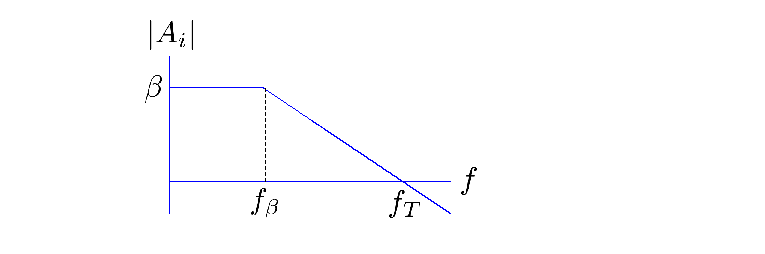
\includegraphics[scale=0.90]{cutoffFreq}
\caption{بلند تعددی بوڈا خط}
\label{شکل_تعددی_ردعمل_بلند_تعددی_بوڈا_خط}
\end{figure}
مساوات \حوالہ{مساوات_تعددی_ردعمل_کسر_دور_افزائش} سے تعدد کی وہ قیمت حاصل کی جا سکتی ہے جس پر قصر دور افزائش کی حتمی قیمت ایک (\عددی{1}) کے برابر ہو۔اس تعدد کو \عددی{\omega_T} لکھتے ہوئے
\begin{align*}
\abs{A_i}=\frac{\beta \omega_{\beta} }{\sqrt{\omega_T^2+\omega_{\beta}^2 }}=1
\end{align*}
سے
\begin{align*}
\beta \omega_{\beta} =\sqrt{\omega_T^2+\omega_{\beta}^2 }
\end{align*}
اور اس کا مربع لیتے ہوئے حل کرتے
\begin{align*}
\beta^2 \omega_{\beta}^2 =\omega_T^2+\omega_{\beta}^2 
\end{align*}
یعنی
\begin{gather}
\begin{aligned}
\omega_T^2 &=\beta^2 \omega_{\beta}^2 -\omega_{\beta}^2 \\
\omega_T &=\omega_{\beta}\sqrt{\beta^2 -1}
\end{aligned}
\end{gather}
چونکہ \عددی{\beta \gg 1} ہوتا ہے لہٰذا
\begin{gather}
\begin{aligned} \label{مساوات_تعددی_ردعمل_افزائش_ضرب_دائرہ}
\omega_T & \approx \beta \omega_{\beta} \\
f_T & \approx \beta f_{\beta}
\end{aligned}
\end{gather}
لکھا جا سکتا ہے۔اس مساوات کے تحت \عددی{f_T} دراصل ٹرانزسٹر کے \عددی{\beta} اور \عددی{f_{\beta}} کا حاصل ضرب ہے۔اسی سے \عددی{f_T} کو ٹرانزسٹر کا \اصطلاح{افزائش ضرب دائرہ کارکردگی}\فرہنگ{افزائش ضرب دائرہ کارکردگی}\حاشیہب{gain bandwidth product}\فرہنگ{gain bandwidth product} کہتے ہیں۔ٹرانزسٹر کے بلند تعددی صلاحیت کو اس کے \اصطلاح{معلوماتی صفحات}\حاشیہب{data sheet} میں بطور \عددی{f_T} پیش کیا جاتا ہے۔یوں کسی بھی اشارے کو بڑھانے کی خاطر استعمال کئے جانے والے ایمپلیفائر کے ٹرانزسٹر کی \عددی{f_T} اس اشارے کی تعدد سے زیادہ ہونا ضروری ہے۔مندرجہ بالا مساوات کو یوں دیکھا جا سکتا ہے کہ اگر دو مختلف ٹرانزسٹروں کی \عددی{f_T} برابر جبکہ ان کے \عددی{\beta} برابر نہ ہوں تب کم \عددی{\beta} والے ٹرانزسٹر کا \عددی{f_{\beta}} زیادہ ہو گا اور یوں یہ نسبتاً زیادہ بلند تعدد کے اشارات کو بڑھانے کی صلاحیت رکھے گا۔

مساوات \حوالہ{مساوات_تعددی_ردعمل_افزائش_ضرب_دائرہ} اور مساوات \حوالہ{مساوات_تعددی_ردعمل_بلند_انقطاعی_بیٹا_تعدد} کو ملاتے ہوئے اور  \عددی{\beta=g_m r_{b'e}} لکھتے ہوئے
\begin{gather}
\begin{aligned}\label{مساوات_تعددی_ردعمل_کپیسٹر_کا_تخمینہ}
f_T &\approx \frac{g_m}{2 \pi \left(C_{b'e}+C_{b'c} \right)}\\
&\approx \frac{g_m}{2 \pi C_{b'e}}
\end{aligned}
\end{gather}
حاصل ہوتا ہے جہاں دوسری قدم پر  \عددی{C_{b'e} \gg C_{b'c}} کی وجہ سے \عددی{C_{b'c}} کو نظر انداز کیا گیا ہے۔

مساوات \حوالہ{مساوات_تعددی_ردعمل_افزائش_ضرب_دائرہ} کے مطابق \عددی{f_T} وہ حتمی بلند تعدد ہے جس تک مشترکہ ایمٹر    ٹرانزسٹر ایمپلیفائر اشارے کا حیطہ بڑھانے کی صلاحیت رکھتا ہے۔اس مساوات کو حاصل کرتے وقت \عددی{C_{b'c}} کے راستے کلکٹر  تک پہنچتے برقی رو کو نظر انداز کیا گیا جس کی وجہ سے حقیقت میں مشترکہ ایمٹر    ٹرانزسٹر ایمپلیفائر  کبھی بھی \عددی{f_T} تعدد کے اشارات  کو نہیں بڑھا سکتا۔

\جزوحصہ{مشترکہ بیس  بلند انقطاعی تعدد}
آئیں مشترکہ بیس  طرز پر استعمال کئے جانے والے ایمپلیفائر کی بلند انقطاعی تعدد حاصل کریں۔بلند انقطاعی تعدد ٹرانزسٹر کے ساتھ بیرونی جڑے مزاحمت وغیرہ پر بھی منحصر ہو گا۔دو مختلف ٹرانزسٹروں کا آپس میں موازنہ کرنے کے لئے یہ ضروری ہے کہ ٹرانزسٹر کے ساتھ بیرونی جڑے پرزوں کے اثر کو شامل نہ کیا جائے۔یوں مشترکہ بیس  بلند تعددی ریاضی نمونے کو استعمال کرتے ہوئے شکل \حوالہ{شکل_تعددی_ردعمل_مشترکہ_قابو_کسر_دور_افزائش} کو زنجیری ضرب سے حل کرتے ہیں۔
\begin{figure}
\centering
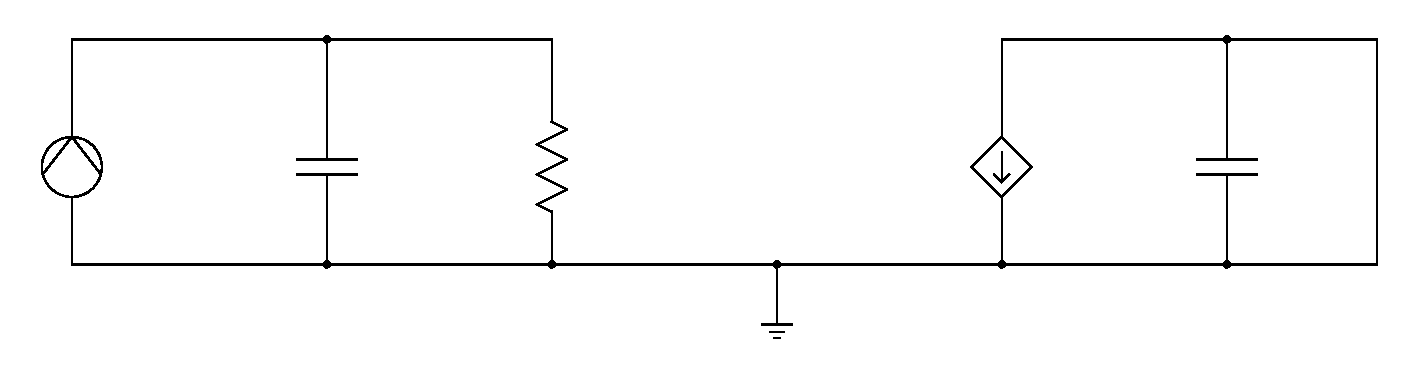
\includegraphics[scale=0.90]{transistorShortCircuitGainCommonBase}
\caption{مشترکہ بیس  قصر دور برقی رو افزائش}
\label{شکل_تعددی_ردعمل_مشترکہ_قابو_کسر_دور_افزائش}
\end{figure}
%
\begin{align*}
\eval{A_i}_{v_{cb} \to 0} &=\frac{i_L}{i_i}=\left(\frac{i_L}{i_c} \right) \left(\frac{i_c}{i_e} \right) \left(\frac{i_e}{i_i} \right)\\
&=\left(-1 \right) \left(\alpha \right) \left(\frac{-\frac{1}{j \omega C_{b'e}}}{r_e+\frac{1}{j \omega C_{b'e}}} \right)\\
&=\frac{\alpha}{j \omega C_{b'e} r_e +1}
\end{align*}
جہاں پہلی قوسین میں منفی کی علامت اس لئے استعمال کئے گئے کہ اس قوسین کے برقی رو \عددی{i_L} اور \عددی{i_c} آپس میں الٹ سمت رکھتے ہیں۔اسی طرح تیسری قوسین میں \عددی{i_e} اور \عددی{i_i} آپس میں الٹ سمت رکھتے ہیں۔مندرجہ بالا مساوات میں
\begin{align*}
C_{b'e} r_e &= \frac{C_{b'e} r_{b'e}}{\beta} =\frac{1}{\beta \omega_{\beta}}=\frac{1}{\omega_T}
\end{align*}
لیتے ہوئے اسے یوں لکھ سکتے ہیں۔
\begin{align}
\eval{A_i}_{v_{cb} \to 0}=\frac{ \alpha}{j\frac{\omega}{\omega_T}+1}
\end{align}
اس مساوات کے مطابق مشترکہ بیس  طرز کے ایمپلیفائر کی \اصطلاح{بلند انقطاعی تعدد}، جسے \عددی{\omega_{\alpha}} پکارا جاتا ہے، ٹرانزسٹر کے \عددی{\omega_T} کے برابر ہوتا ہے یعنی
\begin{align} \label{مساوات_تعددی_ردعمل_مشترکہ_قابو_بلند_انقطاعی_نکتہ}
\omega_{\alpha}=\beta \omega_{\beta}=\omega_T
\end{align}
آپ دیکھ سکتے ہیں کہ مشترکہ بیس  طرز کے ایمپلیفائر انتہائی بلند انقطاعی تعدد رکھتے ہیں۔حقیقت میں \عددی{\omega_T} کے تعدد پر یہاں استعمال کیا گیا ٹرانزسٹر کا بلند تعددی ٹی ریاضی نمونہ درست ثابت نہیں ہوتا لہٰذا مندرجہ بالا مساوات حقیقت میں درست نہیں۔دیکھا یہ گیا ہے کہ
\begin{align}
\omega_{\alpha}=\left(1+\lambda \right) \omega_T
\end{align}
کے برابر ہوتا ہے جہاں \عددی{\lambda} کی قیمت \عددی{\num{0.2}} تا \عددی{\num{1}} ہوتی ہے۔\عددی{\lambda} کی عمومی قیمت \عددی{\num{0.4}} ہے۔
 
\جزوحصہ{\عددی{f_T} کا تجرباتی تخمینہ}
\عددی{f_T} نہایت بلند تعدد ہے جسے ناپنا قدر مشکل ہوتا ہے۔مساوات \حوالہ{مساوات_تعددی_ردعمل_کسر_دور_حتمی_افزائش} کو استعمال کرتے ہوئے \عددی{f_T} کو کم تعدد پر ناپا جا سکتا ہے۔اس مساوات کے مطابق اگر \عددی{A_i} کو تعدد \عددی{f_1} پر ناپا جائے جہاں (\عددی{f_1 \gg f_{\beta}}) ہو مثلاً \عددی{f_1} کی قیمت \عددی{f_{\beta}} کے پانچ یا چھ گنّا ہو تب اسے یوں لکھا جا سکتا ہے۔
\begin{align} \label{مساوات_تعددی_ردعمل_کسر_دور_انقطاعی_تعدد_تخمینہ}
\abs{A_i}_{v_{ce}=0}& \approx \frac{\beta f_{\beta}}{f_1}=\frac{f_T}{f_1}
\end{align}
لہٰذا \عددی{f_1} تعدد پر \عددی{\abs{A_i}} ناپ کر \عددی{f_T} کی قیمت کا تخمینہ لگایا جاتا ہے۔\عددی{f_T} کو استعمال کرتے ہوئے مساوات \حوالہ{مساوات_تعددی_ردعمل_کپیسٹر_کا_تخمینہ} سے \عددی{C_{b'e}}  کی قیمت حاصل کی جاتی ہے۔

\ابتدا{مثال}
ایک ٹرانزسٹر جس کا \عددیء{\beta=200}،\عددی{I_{CQ}=\SI{0.75}{mA}} اور \عددی{f_{\beta}=\SI{1.3}{\mega \hertz}} ہے کا \عددی{\SI{6.5}{\mega \hertz}} کے تعدد  پر \عددی{\abs{A_i}_{v_{ce}=0}} ناپتے ہوئے \عددی{\SI[per=frac,fraction=nice]{41.5}{\ampere \per \ampere}}حاصل ہوتا ہے۔اس کی \عددی{f_T} کا تخمینہ لگاتے ہوئے \عددی{C_{b'e}} حاصل کریں۔

حل: مساوات \حوالہ{مساوات_تعددی_ردعمل_کسر_دور_انقطاعی_تعدد_تخمینہ} کی مدد سے
\begin{align*}
f_T=41.5 \times \SI{6.5}{\mega \hertz} \approx \SI{270}{\mega \hertz}
\end{align*}
حاصل ہوتا ہے۔\عددی{I_{CQ}} سے
\begin{align*}
g_m =\frac{I_{CQ}}{V_T}=\frac{\SI{0.75}{\mA}}{\SI{25}{mV}}=\SI{0.03}{\siemens}
\end{align*}
حاصل ہوتا ہے جسے مساوات \حوالہ{مساوات_تعددی_ردعمل_کپیسٹر_کا_تخمینہ} میں استعمال کرتے ہوئے
\begin{align*}
C_{b'e}=\frac{g_m}{2 \pi f_T}=\frac{0.03}{2 \pi \times 270 \times 10^6} \approx \SI{18}{\pico \farad}
\end{align*}
حاصل ہوتا ہے۔
\انتہا{مثال}
%======
\جزوحصہ{برقی بوجھ کے موجودگی میں بلند تعددی رد عمل}\شناخت{حصہ_تعددی_ردعمل_برقی_بار_موجود_مشترک_مخارج}
شکل \حوالہ{شکل_تعددی_ردعمل_ایمپلیفائر_بلند_تعدد_مساوی_دور} میں مشترکہ ایمٹر    ایمپلیفائر اور اس کا بلند تعدد مساوی دور دکھایا گیا ہے۔یہ بلند تعدد پر استعمال ہونے والے مشترکہ ایمٹر    ایمپلیفائر کی عمومی شکل ہے۔ آئیں پہلے مساوی دور کی سادہ شکل حاصل کریں تا کہ توجہ \اصطلاح{ملر کپیسٹر} پر رکھنی آسان ہو۔پہلے مساوی دور کے داخلی جانب نقطہ دار دائرے میں بند حصے کا مساوی \اصطلاح{تھونن} دور حاصل کرتے ہیں۔شکل \حوالہ{شکل_تعددی_ردعمل_بلند_تعددی_سادہ_دور} الف میں اس حصے کو پیش کیا گیا ہے جہاں تھونن برقی دباو \عددی{v_{th}} اور تھونن مزاحمت \عددی{R_{th}} کی نشاندہی بھی کی گئی ہے۔شکل \حوالہ{شکل_تعددی_ردعمل_بلند_تعددی_سادہ_دور} ب میں مساوی تھونن دور  دکھایا گیا ہے۔متوازی جڑے \عددی{R_1} اور \عددی{R_2} کی کل مزاحمت کو \عددی{R_B} یعنی
\begin{align} \label{مساوات_تعددی_ردعمل_بیس_مزاحمت}
R_B=\frac{R_1 R_2}{R_1+R_2}
\end{align}
لکھتے ہوئے
\begin{align} \label{مساوات_تعددی_ردعمل_تھونن_اجزاء}
v_{th}&=\left(\frac{R_B}{R_S+R_B} \right) v_s \\
R_{th}&=\frac{R_S R_B}{R_S+R_B}
\end{align}
حاصل ہوتے ہیں۔شکل \حوالہ{شکل_تعددی_ردعمل_ایمپلیفائر_بلند_تعدد_مساوی_دور} ب میں \عددی{R_C} اور \عددی{R_L'} متوازی جڑے ہیں۔ان کے کل مزاحمت کو \عددی{R_L} لکھتے ہیں یعنی
\begin{align} \label{مساوات_تعددی_ردعمل_اصل_بار}
R_L=\frac{R_C R_L'}{R_C+R_L'}
\end{align}
\عددی{C_{b'c}} پر نظر ڈالنے سے ہم دیکھتے ہیں کہ اس کے ایک جانب \عددی{v_{b'e}} اور دوسری جانب \عددی{v_o} برقی دباو ہے۔یوں \عددی{C_{b'c}} کے ملر کپیسٹر حاصل کئے جا سکتے ہیں۔ان تبدیلیوں کی مدد سے شکل \حوالہ{شکل_تعددی_ردعمل_بلند_تعددی_سادہ_دور} پ کا سادہ دور حاصل ہوتا ہے جہاں \عددی{C_{b'c}} کو مسئلہ ملر کی مدد سے \عددی{C_M} اور \عددی{C_M'} جڑوا کپیسٹروں میں تبدیل کر دیا گیا ہے۔
\begin{figure}
\centering
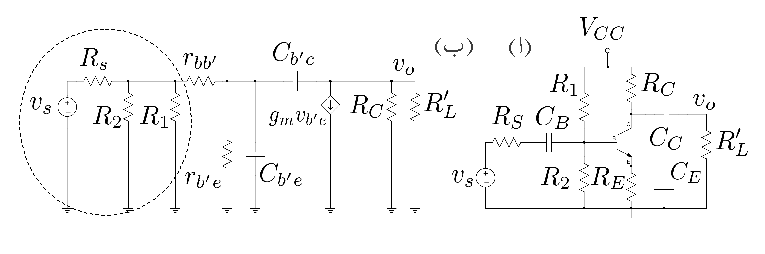
\includegraphics[scale=0.90]{highFreqResponseIncludingMillerCapacitorA}
\caption{ایمپلیفائر اور اس کا بلند تعدد مساوی دور}
\label{شکل_تعددی_ردعمل_ایمپلیفائر_بلند_تعدد_مساوی_دور}
\end{figure}
%
\begin{figure}
\centering
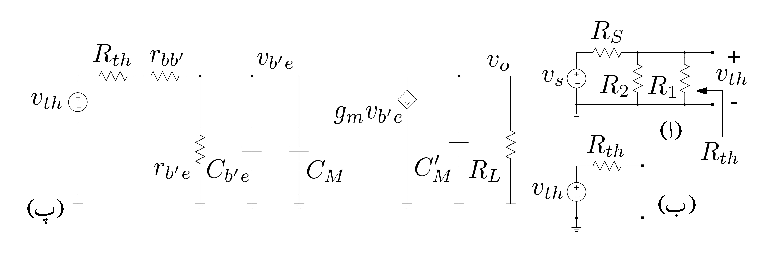
\includegraphics[scale=0.90]{highFreqResponseIncludingMillerCapacitorB}
\caption{بلند تعددی سادہ دور}
\label{شکل_تعددی_ردعمل_بلند_تعددی_سادہ_دور}
\end{figure}
شکل \حوالہ{شکل_تعددی_ردعمل_ایمپلیفائر_بلند_تعدد_مساوی_دور} پ کے طرز پر ادوار میں عموماً \عددی{C_M'} کی برقی رکاوٹ متوازی جڑے مزاحمت \عددی{R_L} سے بہت زیادہ ہوتی ہے یعنی
\begin{align}
\frac{1}{\omega C_M'} \gg R_L
\end{align}
لہٰذا \عددی{C_M'}  کو نظر انداز کیا جاتا ہے۔ایسا کرنے سے شکل \حوالہ{شکل_تعددی_ردعمل_بلند_تعددی_سادہ_دور_الف} حاصل ہوتا ہے۔آئیں دیکھیں کہ مندرجہ بالا مساوات کیوں درست ثابت ہوتا ہے۔

کسی بھی ایمپلیفائر کو بلند اور پست انقطاعی تعدد کے مابین درمیانی تعدد کے خطے میں استعمال کیا جاتا ہے جہاں یہ داخلی اشارے کا حیطہ بڑھانے کی صلاحیت رکھتا ہے۔اس خطے میں ٹرانزسٹر کا پست تعددی ریاضی نمونہ استعمال کیا جاتا ہے۔اگر شکل \حوالہ{شکل_تعددی_ردعمل_بلند_تعددی_سادہ_دور} پ میں پست تعددی ریاضی نمونہ استعمال کیا جائے تو ملر کپیسٹر کے حصول میں درکار \عددی{A_V} کی قیمت
\begin{align}
A_V&=\frac{v_o}{v_{be}}=-g_m R_L
\end{align}
ہو گی جہاں \عددی{v_{b'e}} کی جگہ \عددی{v_{be}} کا استعمال کیا گیا ہے۔اس قیمت کو استعمال کرتے ہوئے مساوات \حوالہ{مساوات_تعددی_ردعمل_ملر_کپیسٹر} اور \حوالہ{مساوات_تعددی_ردعمل_ملر_کپیسٹر_الف} سے
\begin{align} \label{مساوات_تعددی_ردعمل_ملر_کپیسٹر_قیمت}
C_M&=C_{b'c}\left(1+g_m R_L \right)\\
C_M'&=C_{b'c} \left(1+\frac{1}{g_m R_L} \right) 
\end{align}
حاصل ہوتے ہیں۔درمیانی تعدد کے خطے میں ایمپلیفائر کی افزائش کی حتمی قیمت  \عددی{\abs{A_V}} ایک (\عددی{1}) سے کئی گنّا زیادہ ہوتی ہے (یعنی  \عددی{{g_m R_L} \gg 1} ) لہٰذا
\begin{align}
C_M' \approx C_{b'c}
\end{align}
ہو گا۔\عددی{C_{b'c}} کی قیمت انتہائی کم ہوتی ہے۔یوں اس کے برقی رکاوٹ کی حتمی قیمت برقی بوجھ سے بہت زیادہ ہو گی یعنی 
\begin{align}
\abs{\frac{1}{j \omega C_{b'c}}} \gg R_L
\end{align}
لہٰذا \عددی{C_{b'c}} کو نظر انداز کیا جا سکتا ہے۔بلند تعدد ایمپلیفائر  حل کرتے وقت \عددی{C_M} کو استعمال جبکہ \عددی{C_M'} کو استعمال نہیں کیا جاتا۔یہاں اس بات کو ذہن نشین کر لیں کہ ایمپلیفائر کی افزائش بڑھانے سے \عددی{C_M} کی قیمت بھی بڑھتی ہے۔
\begin{figure}
\centering
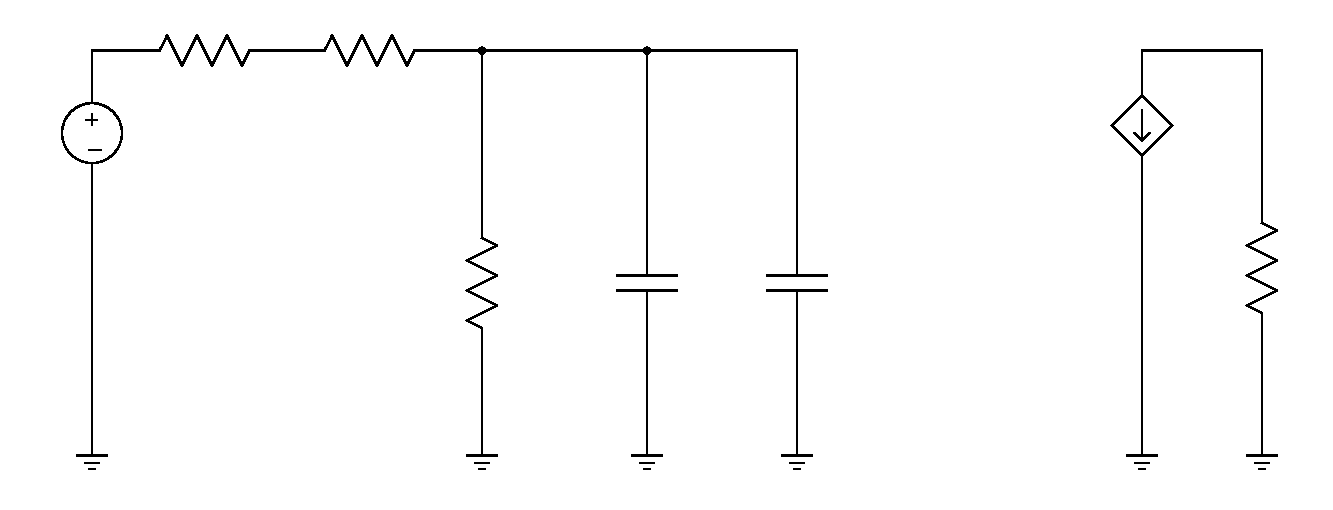
\includegraphics[scale=0.90]{highFreqResponseIncludingMillerCapacitorC}
\caption{ملر کپیسٹر کے اثرات}
\label{شکل_تعددی_ردعمل_بلند_تعددی_سادہ_دور_الف}
\end{figure}

آئیں شکل \حوالہ{شکل_تعددی_ردعمل_بلند_تعددی_سادہ_دور_الف} کو \اصطلاح{کرخوف کے قوانین} استعمال کرتے ہوئے حل کرتے ہیں۔شکل میں \عددیء{r_{b'e}}، \عددی{C_{b'e}} اور \عددی{C_M} متوازی جڑے ہیں۔ان کی کل برقی رکاوٹ کو \عددی{Z} سے ظاہر کرتے ہیں۔یوں
\begin{align*}
\frac{1}{Z}&=s\left(C_{b'e}+C_M \right)+\frac{1}{r_{b'e}}
\end{align*}
سے
\begin{align}
Z=\frac{r_{b'e}}{s \left(C_{b'e}+C_M \right) r_{b'e}+1}
\end{align}
حاصل ہوتا ہے۔زنجیری ضرب سے
\begin{align*}
A_v'&=\frac{v_o}{v_{th}}=\left(\frac{v_o}{i_c}\right) \left(\frac{i_c}{v_{b'e}}\right) \left(\frac{v_{b'e}}{v_{th}}\right)\\
&=\left(-R_L \right) \left(g_m \right) \left(\frac{Z}{R_{th}+r_{bb'}+Z} \right)
\end{align*}
حاصل ہوتا ہے۔اس میں \عددی{Z} کی قیمت استعمال کرتے ہوئے حل کرتے ہیں۔
\begin{align*}
A_v'&=-R_L g_m \left(\frac{\frac{r_{b'e}}{s \left(C_{b'e}+C_M \right) r_{b'e}+1}}{R_{th}+r_{bb'}+\frac{r_{b'e}}{s \left(C_{b'e}+C_M \right) r_{b'e}+1}} \right)\\
&=\frac{-R_L g_m r_{b'e}}{\left[s \left(C_{b'e}+C_M \right) r_{b'e}+1 \right] \left(R_{th}+r_{bb'} \right) +r_{b'e}}\\
&=\frac{-R_L g_m r_{b'e}}{s \left(C_{b'e}+C_M \right) r_{b'e} \left(R_{th}+r_{bb'} \right) +R_{th}+r_{bb'}+r_{b'e}}\\
&=\frac{-R_L g_m r_{b'e}}{\left(C_{b'e}+C_M \right) r_{b'e} \left(R_{th}+r_{bb'} \right) \left[s+\frac{R_{th}+r_{bb'}+r_{b'e}}{\left(C_{b'e}+C_M \right) r_{b'e} \left(R_{th}+r_{bb'} \right)} \right]}
\end{align*}
جسے
\begin{align}  \label{مساوات_تعددی_ردعمل_بلند_تعددی_تھونن}
A_v'&=-\left[\frac{g_m R_L}{\left(C_{b'e}+C_M \right) \left(R_{th}+r_{bb'} \right)}\right] \left(\frac{1}{s+\omega_H} \right)
\end{align}
لکھا جا سکتا ہے جہاں
\begin{gather}
\begin{aligned}\label{مساوات_تعددی_ردعمل_بلند_انقطاعی_تعدد_ٹھیک_ٹھیک}
\omega_H&=\frac{R_{th}+r_{bb'}+r_{b'e}}{\left(C_{b'e}+C_M \right) r_{b'e} \left(R_{th}+r_{bb'} \right)}\\
&=\frac{1}{\left[r_{b'e} \mathbin{\|} \left(R_{th}+r_{bb'} \right) \right] \left(C_{b'e}+C_M \right)}\\
&\frac{1}{R_m \left(C_{b'e}+C_{M} \right)}
\end{aligned}
\end{gather}
ہے۔\عددی{\omega_H} کی مساوات جانی پہچانی شکل یعنی \عددی{\frac{1}{R_m C}} ہے جہاں \عددی{C} متوازی جڑے کپیسٹر \عددی{C_{b'e}} اور \عددی{C_M} کی کل کپیسٹنس \عددی{\left(C_{b'e}+C_M \right)} ہے جبکہ \عددی{R_m} اس کپیسٹر کے ساتھ کل متوازی جڑی مزاحمت ہے۔شکل \حوالہ{شکل_تعددی_ردعمل_بلند_تعددی_سادہ_دور_الف} میں \عددی{v_s} کو قصر دور کرتے ہوئے \عددی{r_{b'e}} کے ساتھ متوازی جڑے \عددی{\left(R_{th}+r_{bb'} \right)}  کی کل مزاحمت \عددی{R_m} ہے یعنی
\begin{align*}
\frac{1}{R_m}&=\frac{1}{r_{b'e}}+\frac{1}{R_{th}+r_{bb'}} \\
R_m&=\frac{ r_{b'e} \left(R_{th}+r_{bb'} \right)}{R_{th}+r_{bb'}+r_{b'e}}
\end{align*}
جسے یوں بھی لکھا جا سکتا ہے۔
\begin{align*}
R_m&= r_{b'e} \mathbin{\|}\left(R_{th}+r_{bb'} \right)
\end{align*}
چونکہ  \عددی{R_{th}} کی قیمت \عددی{r_{b'e}} اور \عددی{r_{bb'}} سے بہت زیادہ ہوتی ہے یعنی
\begin{align*}
R_{th} & \gg r_{bb'}\\
R_{th} & \gg r_{b'e}
\end{align*}
لہٰذا
\begin{align*}
R_m \approx r_{b'e}
\end{align*}
کے برابر ہو گا اور یوں
\begin{gather}
\begin{aligned} \label{مساوات_تعددی_ردعمل_بلند_انقطاعی_تعدد}
\omega_H &= \frac{1}{\left(C_{b'e}+C_M \right) r_{b'e}} \\
f_H& = \frac{1}{2 \pi \left(C_{b'e}+C_M \right) r_{b'e}} 
\end{aligned}
\end{gather}
ہو گا۔\عددی{\omega_H} کا مساوات \حوالہ{مساوات_تعددی_ردعمل_کسر_دور_انقطاعی_تعدد} میں دئے \عددی{\omega_{\beta}} سے موازنہ کرتے ہیں۔
\begin{align} \label{مساوات_تعددی_ردعمل_بلند_تعدد_شرح}
\frac{\omega_{\beta}}{\omega_H}=\frac{\left(\frac{1}{C_{b'e} r_{b'e}} \right)}{\left [\frac{1}{\left(C_{b'e}+C_M \right) r_{b'e}} \right]}=\frac{C_{b'e}+C_M}{C_{b'e}}=1+\frac{C_M}{C_{b'e}}
\end{align}
آپ دیکھ سکتے ہیں کہ مشترکہ ایمٹر       ایمپلیفائر کا بلند انقطاعی تعدد \عددی{\omega_H}  ہے  لہٰذا ایمپلیفائر کی افزائش  \عددی{\omega_{\beta}} تعدد پر نہایت کم ہو گی۔

\عددی{A_v=\frac{v_o}{v_s}} کو مساوات \حوالہ{مساوات_تعددی_ردعمل_بلند_تعددی_تھونن} اور مساوات \حوالہ{مساوات_تعددی_ردعمل_تھونن_اجزاء} کی مدد سے یوں حاصل کر سکتے ہیں۔
\begin{align*}
A_v&=\frac{v_o}{v_s}=\left (\frac{v_o}{v_{th}} \right)  \left(\frac{v_{th}}{v_s} \right)\\
&=-\left[\frac{g_m R_L}{\left(C_{b'e}+C_M \right) \left(R_{th}+r_{bb'} \right)}\right] \left(\frac{R_B}{R_S+R_B} \right)\left(\frac{1}{s+\omega_H} \right) \\
&=-\left[\frac{g_m R_L}{\omega_H \left(C_{b'e}+C_M \right) \left(R_{th}+r_{bb'} \right)}\right] \left(\frac{R_B}{R_S+R_B} \right)\left(\frac{1}{1+\frac{s}{\omega_H}} \right)\\
&=-\left(\frac{g_m R_m R_L}{R_{th}+r_{bb'}}\right) \left(\frac{R_B}{R_S+R_B} \right)\left(\frac{1}{1+\frac{s}{\omega_H}} \right)
\end{align*}
جہاں دوسرے قدم پر مساوات \حوالہ{مساوات_تعددی_ردعمل_بلند_انقطاعی_تعدد_ٹھیک_ٹھیک} کا استعمال کیا گیا۔\عددی{R_m \approx r_{b'e}} کی صورت میں اسے یوں لکھا جا سکتا ہے۔
\begin{align*}
A_v \approx -\left(\frac{g_m r_{b'e} R_L}{R_{th}+r_{bb'}}\right) \left(\frac{R_B}{R_S+R_B} \right)\left(\frac{1}{1+\frac{s}{\omega_H}} \right)
\end{align*}
\عددی{g_m r_{b'e}=\beta} لکھتے ہوئے
\begin{align}  \label{مساوات_تعددی_ردعمل_مکمل_افزائش_مساوات}
A_v \approx -\left(\frac{\beta R_L}{R_{th}+r_{bb'}}\right) \left(\frac{R_B}{R_S+R_B} \right)\left(\frac{1}{1+\frac{s}{\omega_H}} \right)
\end{align}
حاصل ہوتا ہے۔اس مساوات سے درمیانی تعدد پر \عددی{\abs{A_{vD}}_{\omega \ll \omega_H}} حاصل کرتے ہیں۔
\begin{align} \label{مساوات_تعددی_ردعمل_درمیانی_تعدد_حتمی_افزائش}
\abs{A_{vD}}_{\omega \ll \omega_H}&=-\left(\frac{\beta R_L}{R_{th}+r_{bb'}}\right) \left(\frac{R_B}{R_S+R_B} \right)
\end{align}
%=============================

\ابتدا{مثال}
شکل \حوالہ{شکل_تعددی_ردعمل_ایمپلیفائر_بلند_تعدد_مساوی_دور} میں
\begin{align*}
V_{CC}=\SI{15}{V} \hspace{1cm} R_1=\SI{7}{\kilo \ohm} \hspace{1cm} R_2=\SI{2.8}{\kilo \ohm}\\
R_C=\SI{650}{\ohm} \hspace{1cm} R_L'=\SI{100}{\ohm}  \hspace{1cm} R_E=\SI{260}{\ohm} \\
C_{b'c}=\SI{2}{\pico \farad} \hspace{1cm} C_{b'e}=\SI{220}{\pico \farad} \hspace{1cm} r_{bb'}=\SI{20}{\ohm}\\
\beta=\num{75} \hspace{1cm} R_S=\SI{1.2}{\kilo \ohm}
\end{align*}
لیتے ہوئے \عددیء{I_{CQ}\approx \SI{12.5}{\milli \ampere}}، \عددی{g_m =\SI{0.5}{\siemens}} اور \عددی{r_{b'e}=\SI{150}{\ohm}} حاصل ہوتے ہیں۔اس ایمپلیفائر کی درمیانی تعدد پر افزائش \عددی{A_v} اور بلند انقطاعی تعدد \عددی{f_H} حاصل کریں۔

حل:حصہ \حوالہ{حصہ_تعددی_ردعمل_برقی_بار_موجود_مشترک_مخارج} میں اسی کو کرخوف کے قوانین کی مدد سے حل کیا گیا۔اس مثال کو مسئلہ نارٹن اور مسئلہ تھونن کے بار بار استعمال سے حل کرتے ہیں۔

\عددی{R_C \mathbin{\|} R_L'} کو \عددی{R_L} لکھتے ہوئے
\begin{align*}
R_L=\frac{650 \times 100}{650+100}=\SI{87}{\ohm}
\end{align*}
حاصل ہوتا ہے۔شکل \حوالہ{شکل_تعددی_ردعمل_ایمپلیفائر_بلند_تعدد_مساوی_دور} ب سے مسئلہ ملر کی مدد سے شکل \حوالہ{شکل_تعددی_ردعمل_ماسفیٹ_مشترکہ_مخارج_نارٹن_تھونن_بار_بار} الف حاصل ہوتا ہے جہاں
\begin{align*}
C&=C_{b'e}+C_M\\
&=C_{b'e}+\left(1+g_mR_L \right) C_{b'c}\\
&=220 \times 10^{-12}+\left(1+0.5 \times 87 \right) \times 2 \times 10^{-12}\\
&=\SI{220}{\pico \farad}+\SI{89}{\pico \farad}\\
&=\SI{309}{\pico \farad}
\end{align*}
کے برابر ہے اور  \عددی{R_1 \mathbin{\|}R_2} کو \عددی{R_B} کہا گیا ہے یعنی
\begin{align*}
R_B=\frac{R_1 R_2}{R_1+R_2}=\frac{7000 \times 2800}{7000+2800}=\SI{2}{\kilo \ohm}
\end{align*}
%
\begin{figure}
\centering
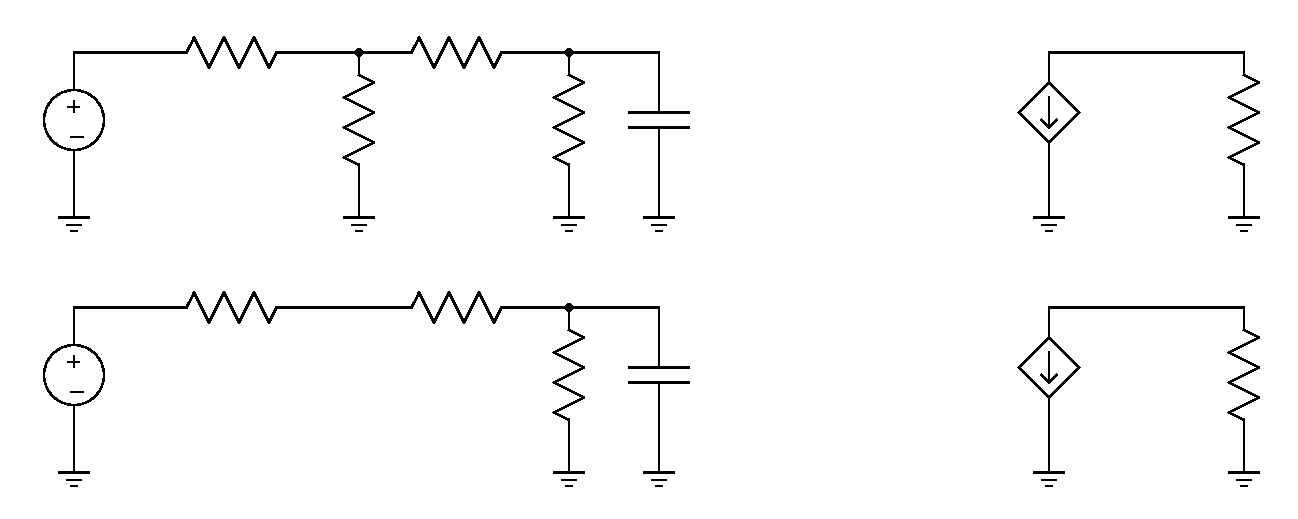
\includegraphics[scale=0.90]{highFreqResponseIncludingMillerCapacitorNortonTheveninUsage}
\caption{مسئلہ نارٹن اور مسئلہ تھونن کے بار بار استعمال سے دور کا حل}
\label{شکل_تعددی_ردعمل_ماسفیٹ_مشترکہ_مخارج_نارٹن_تھونن_بار_بار}
\end{figure}
اس شکل میں نقطہ دار لکیر کے بائیں جانب کا مساوی تھونن دور لیتے ہوئے شکل \حوالہ{شکل_تعددی_ردعمل_ماسفیٹ_مشترکہ_مخارج_نارٹن_تھونن_بار_بار} ب حاصل ہوتا ہے جہاں تھونن مساوی مقدار
\begin{align*}
\left(\frac{R_B}{R_S+R_B}\right) v_s &=0.625 v_s \hspace{5mm} \text{\RL{تھونن دباو}}\\
R_S \mathbin{\|} R_B &= \SI{750}{\ohm} \hspace{5mm}\text{\RL{تھونن مزاحمت}}
\end{align*}
ہیں۔شکل \حوالہ{شکل_تعددی_ردعمل_ماسفیٹ_مشترکہ_مخارج_نارٹن_تھونن_بار_بار} ب کے نقطہ دار لکیر سے بائیں جانب حصے کا اب مساوی نارٹن دور لیتے ہیں جسے شکل \حوالہ{شکل_تعددی_ردعمل_ماسفیٹ_مشترکہ_مخارج_نارٹن_تھونن_بار_بار_الف} الف میں دکھایا گیا ہے جہاں نارٹن مساوی برقی رو 
\begin{align*}
\frac{0.625 v_s}{R_B'}=\frac{0.625}{770}v_s
\end{align*}
کے برابر ہے۔
\begin{figure}
\centering
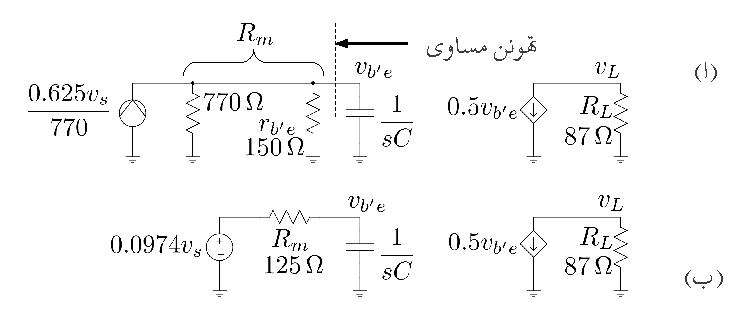
\includegraphics[scale=0.90]{highFreqResponseIncludingMillerCapacitorNortonTheveninUsageA}
\caption{مسئلہ نارٹن اور مسئلہ تھونن کے بار بار استعمال سے دور کا حل}
\label{شکل_تعددی_ردعمل_ماسفیٹ_مشترکہ_مخارج_نارٹن_تھونن_بار_بار_الف}
\end{figure}
شکل \حوالہ{شکل_تعددی_ردعمل_ماسفیٹ_مشترکہ_مخارج_نارٹن_تھونن_بار_بار_الف} الف میں نقطہ دار لکیر کے بائیں جانب حصے کا تھونن مساوی دور لیتے ہوئے شکل  ب حاصل ہوتا ہے۔شکل \حوالہ{شکل_تعددی_ردعمل_ماسفیٹ_مشترکہ_مخارج_نارٹن_تھونن_بار_بار_الف} ب کو دیکھ کر \عددی{v_{b'e}} کی مساوات لکھی جا سکتی ہے۔
\begin{align*}
v_{b'e}&=0.101 v_s \left(\frac{\frac{1}{sC}}{125+\frac{1}{sC}}\right)=0.101 v_s \left(\frac{1}{125 \times s C+1}\right)\\
&=\frac{0.101 v_s }{1+\frac{j \omega}{26 \times 10^6}}=\frac{0.101 v_s }{1+\frac{j f}{4 \times 10^6}}
\end{align*}
زنجیری ضرب سے
\begin{align*}
A_v=\frac{v_L}{v_s}&=\frac{v_L}{i_c} \times \frac{i_c}{v_{b'e}} \times \frac{v_{b'e}}{v_s}\\
&=-87 \times 0.5 \times \left(\frac{0.101}{1+\frac{j f}{4 \times 10^6}}\right)\\
&=\frac{-4.4}{1+\frac{j f}{4 \times 10^6}}
\end{align*}
لکھا جا سکتا ہے۔بلند انقطاعی تعدد تقریباً \عددی{f_H=\SI{4}{\mega \hertz}} جبکہ درمیانی تعدد کی افزائش \عددی{A_{vD}=\SI{-4.4}{\volt \per \volt}} ہے۔ 
\انتہا{مثال}
%==================
\جزوحصہ{مشترکہ سورس ماسفیٹ ایمپلیفائر کا بلند تعددی ردِ عمل}
شکل \حوالہ{شکل_تعددی_ردعمل_ماسفیٹ_مشترکہ_مخارج} الف میں ماسفیٹ ایمپلیفائر اور شکل  ب میں اسی کا مساوی بلند تعددی دور دکھایا گیا ہے جس میں ماسفیٹ کا بلند تعددی ریاضی نمونہ استعمال کیا گیا ہے۔ماسفیٹ کا بلند تعددی ریاضی نمونہ ماسفیٹ کے پست تعددی ریاضی نمونے میں \عددی{C_{gs}} اور \عددی{C_{gd}} اندرونی کپیسٹر کی شمولیت سے حاصل کیا گیا ہے۔شکل \حوالہ{شکل_تعددی_ردعمل_ماسفیٹ_مشترکہ_مخارج} ب اور شکل \حوالہ{شکل_تعددی_ردعمل_ایمپلیفائر_بلند_تعدد_مساوی_دور} ب  تقریباً یکساں صورت رکھتے ہیں۔ماسفیٹ کے ریاضی نمونے میں  \عددی{C_{gs} \gg  C_{gd}} ہوتا ہے۔پست تعددی ماسفیٹ کے \عددی{C_{gs}} کی قیمت \عددی{\SI{50}{\pico \farad}} جبکہ بلند تعددی ماسفیٹ کی \عددی{\SI{5}{\pico \farad}} سے بھی کم ہوتی ہے۔پست تعددی ماسفیٹ کے \عددی{C_{gd}} کی قیمت \عددی{\SI{5}{\pico \farad}} جبکہ بلند تعددی ماسفیٹ کی \عددی{\SI{0.5}{\pico \farad}} سے بھی کم ہوتی ہے۔
\begin{align*}
R_L&=\frac{R_L' R_D}{R_L'+R_D}\\
R_G&=\frac{R_1 R_2}{R_1+R_2}
\end{align*}
لیتے ہوئے نقطہ دار دائرے میں بند حصے کا تھونن مساوی دور حاصل کرتے ہیں۔
\begin{align*}
R_{th}&=\frac{R_i  R_G}{R_i+R_G}\\
v_{th}&=\left(\frac{R_G}{R_i+R_G} \right) v_i
\end{align*}
%
\begin{figure}
\centering
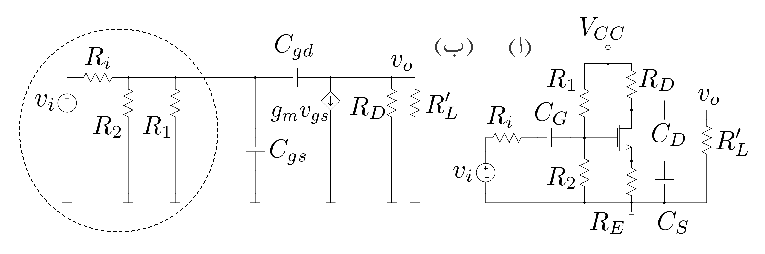
\includegraphics[scale=0.90]{highFreqResponseMosfetAmplifier}
\caption{ماسفیٹ ایمپلیفائر اور اس کا بلند تعددی مساوی دور}
\label{شکل_تعددی_ردعمل_ماسفیٹ_مشترکہ_مخارج}
\end{figure}
\عددی{C_{gd}} کا ملر کپیسٹر استعمال کرتے ہوئے شکل \حوالہ{شکل_تعددی_ردعمل_ماسفیٹ_مشترکہ_مخارج_ملر} حاصل ہوتا ہے۔آئیں اس مرتبہ \عددی{C_M'} کو نظر انداز نہ کرتے ہوئے دور کو حل کریں۔متوازی جڑے \عددی{R_L} اور \عددی{C_M'} کی برقی رکاوٹ کو \عددی{Z_L} لکھتے ہوئے
\begin{align*}
\frac{1}{Z_L}&=j \omega C_M' +\frac{1}{R_L}\\
Z_L&=\frac{R_L}{j \omega C_M' R_L+1}
\end{align*}
حاصل ہوتا ہے۔یوں
\begin{align*}
\frac{v_o}{v_{th}}&=\left(\frac{v_o}{i_d} \right) \left(\frac{i_d}{v_{gs}} \right) \left(\frac{v_{gs}}{v_{th}} \right)\\
&=\left(- Z_L \right) \left(g_m \right) \left(\frac{\frac{1}{j \omega (C_{gs}+C_M)}}{R_{th}+\frac{1}{j \omega (C_{gs}+C_M)}} \right)\\
&=-\left(\frac{g_m R_L}{j \omega C_M' R_L+1} \right) \left(\frac{1}{j \omega (C_{gs}+C_M) R_{th}+1} \right)
\end{align*}
%
\begin{figure}
\centering
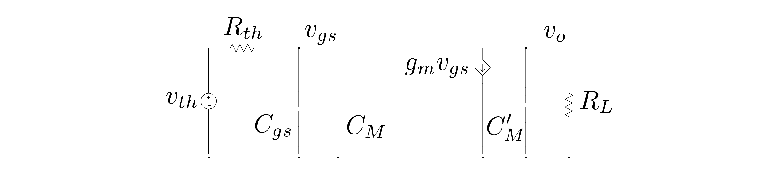
\includegraphics[scale=0.90]{highFreqResponseMosfetAmplifierA}
\caption{ماسفیٹ ایمپلیفائر میں ملر کپیسٹر کا اثر}
\label{شکل_تعددی_ردعمل_ماسفیٹ_مشترکہ_مخارج_ملر}
\end{figure}
اس میں
\begin{align}
\omega_H'&=\frac{1}{C_M' R_L}\\
\omega_H&=\frac{1}{\left(C_{gs}+C_M\right) R_{th}}
\end{align}
لیتے ہوئے
\begin{align}
\frac{v_o}{v_{th}}&=-\left(\frac{g_m R_L}{j \frac{\omega}{\omega_H'}+1} \right) \left(\frac{1}{j \frac{\omega}{\omega_H} +1} \right)
\end{align}
لکھا جا سکتا ہے۔

آپ دیکھ سکتے ہیں کہ \عددی{C_M'} سے \عددی{\omega_H'} حاصل ہوتا ہے جسے گزشتہ حصے میں نظر انداز کیا گیا تھا۔حقیقت میں \عددی{\omega_H' \gg \omega_H} ہوتا ہے لہٰذا ماسفیٹ      ایمپلیفائر میں بھی \عددی{C_M'} کی موجودگی کو نظر انداز کیا جاتا ہے۔یوں \عددی{\omega \ll \omega_H'} تعدد پر چلتے ہوئے کل افزائش یوں لکھی جائے گی۔
\begin{align}
A_v&=\left(\frac{v_o}{v_{th}} \right) \left( \frac{v_{th}}{v_i}\right)=-\left(\frac{g_m R_L}{j \frac{\omega}{\omega_H} +1} \right) \left(\frac{R_G}{R_G+R_i} \right)
\end{align}
اس مساوات کے مطابق بلند انقطاعی تعدد کا دارومدار \عددی{R_{th}} پر ہے۔آئیں دیکھیں کہ ماسفیٹ کی بلند ترین انقطاعی تعدد کس صورت حاصل ہو گی۔ایسا کرنے کی خاطر شکل \حوالہ{شکل_تعددی_ردعمل_ماسفیٹ_مشترکہ_مخارج} میں \عددی{R_i=\SI{0}{\ohm}} لیتے  ہوئے اس کا مساوی دور حاصل کرتے ہیں جسے شکل \حوالہ{شکل_تعددی_ردعمل_ماسفیٹ_بلند_ترین_انقطاعی} میں دکھایا گیا ہے جہاں \عددی{r_o} کو بھی شامل کیا گیا ہے۔اس شکل میں چونکہ \عددیء{R_1}، \عددی{R_2} اور \عددی{C_{gs}} تینوں داخلی اشارہ \عددی{v_i} کے متوازی جڑے ہیں لہٰذا گیٹ پر \عددی{v_i} ہی پایا جائے۔یوں \عددی{v_{gs}=v_i} کے برابر ہو گا۔ \عددی{v_o} جوڑ پر کرخوف کے قانون برائے برقی رو کے مدد سے ہم لکھ سکتے ہیں
\begin{figure}
\centering
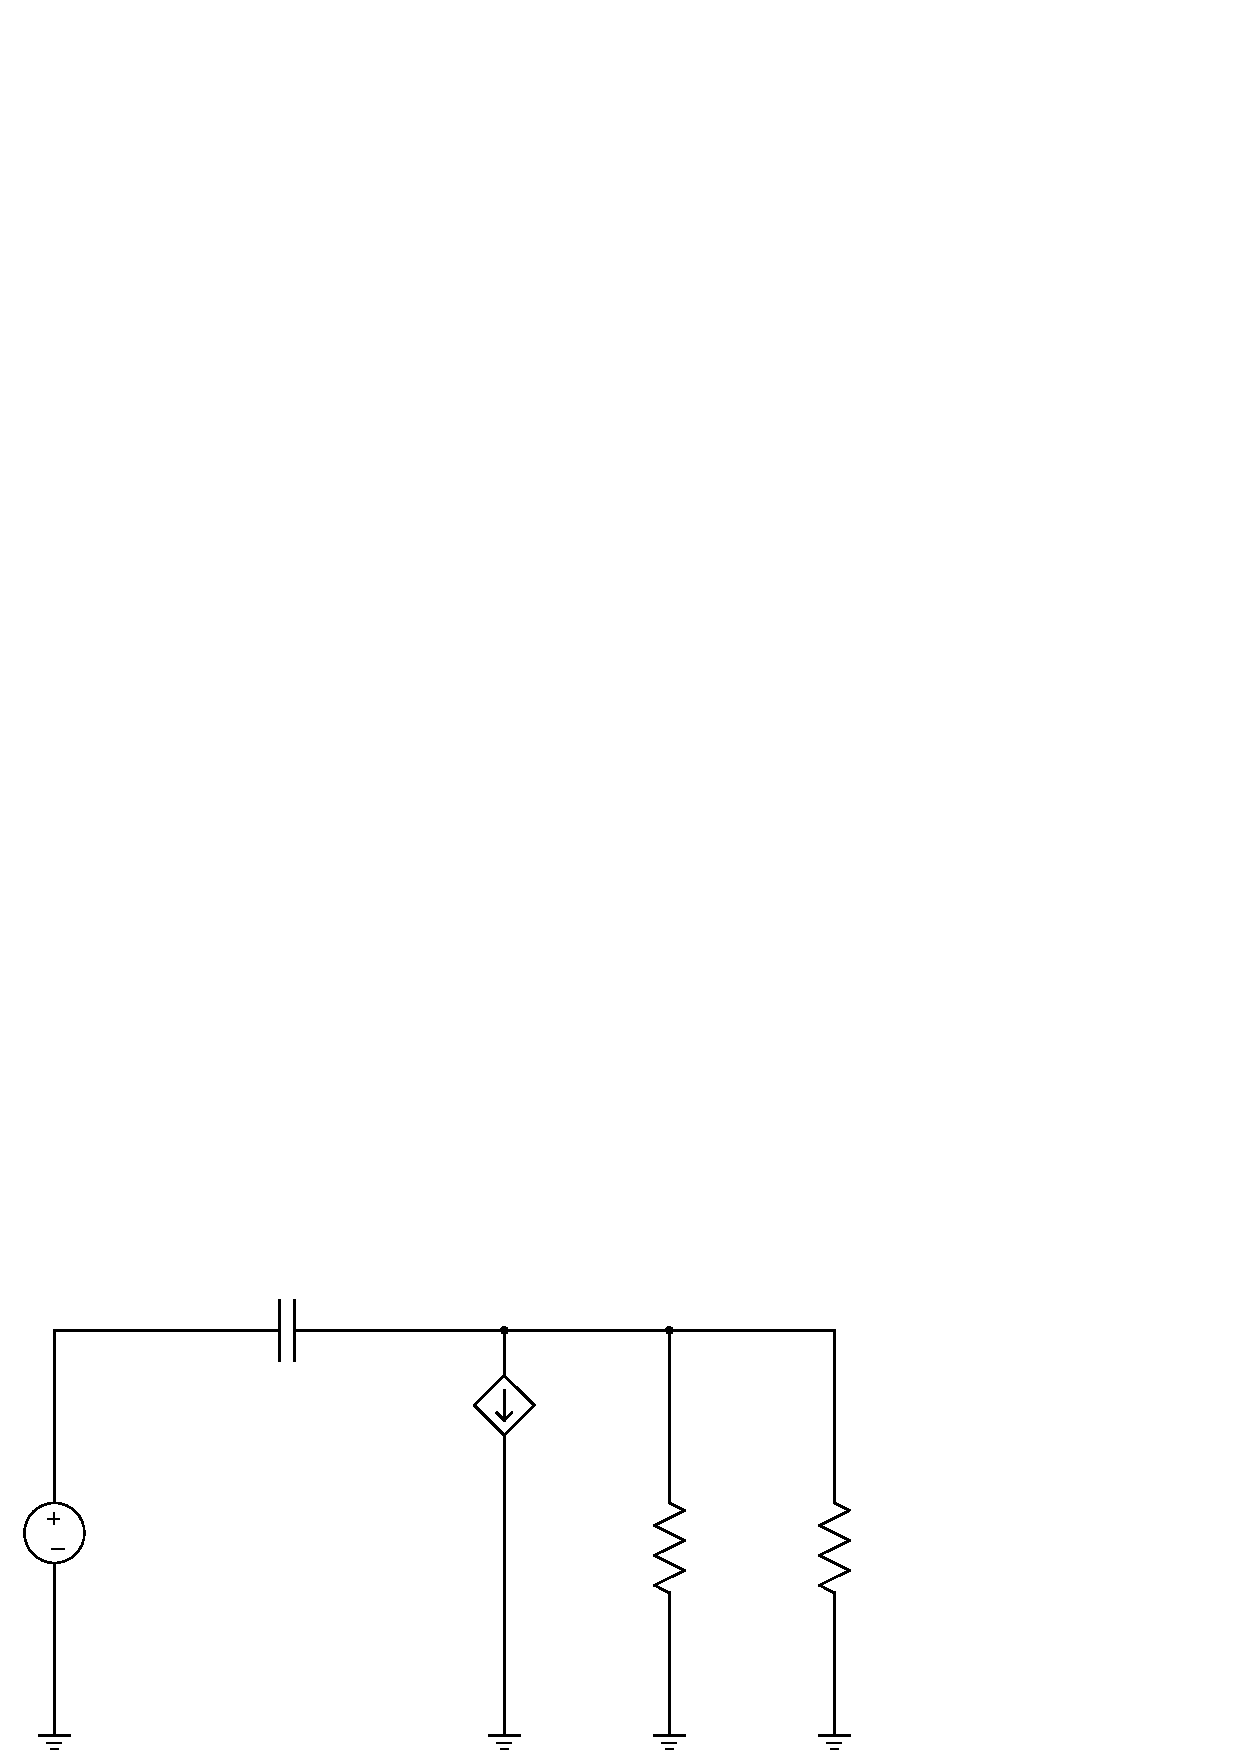
\includegraphics[scale=0.90]{highFreqResponseMosfetAmplifierB}
\caption{بلند ترین ممکنہ انقطاعی تعدد کا حصول}
\label{شکل_تعددی_ردعمل_ماسفیٹ_بلند_ترین_انقطاعی}
\end{figure}
%
\begin{align*}
\frac{v_o-v_i}{\frac{1}{j \omega C_{gd}}}+g_m v_i+\frac{v_o}{\frac{R_L r_o}{R_L+r_o}}=0\\
\frac{v_o}{v_i}=\left(\frac{R_L r_o}{r_L+r_o} \right)\left[\frac{j \omega C_{gd}-g_m}{1+\omega C_{gd} \left(\frac{R_L r_o}{R_L+r_o} \right)} \right]
\end{align*}
یعنی
\begin{align}
A_v=\frac{v_o}{v_i}=\left(\frac{g_m R_L r_o}{r_L+r_o} \right)\left[-1+\frac{j \frac{\omega C_{gd}}{g_m}}{1+j\omega C_{gd} \left(\frac{R_L r_o}{R_L+r_o} \right)} \right]
\end{align}
جس میں
\begin{align}
\omega_s&=\frac{g_m}{C_{gd}}\\
\omega_H&=\frac{1}{C_{gd} \left(\frac{R_L r_o}{R_L+r_o} \right)}
\end{align}
لیتے ہوئے
\begin{align} \label{مساوات_تعددی_ردعمل_مشترکہ_مخارج_ماسفیٹ_ایمپلیفائر_افزائش}
A_v=\left(\frac{g_m R_L r_o}{r_L+r_o} \right)\left[\frac{-1+j \frac{\omega}{\omega_s}}{1+j \frac{\omega}{\omega_H}} \right]
\end{align}
حاصل ہوتا ہے۔اس مساوات میں \عددی{\omega_s \gg \omega_H} ہوتا ہے یعنی
\begin{align*}
\frac{g_m}{C_{gd}} \gg \frac{1}{C_{gd} \left(\frac{R_L r_o}{R_L+r_o} \right)}
\end{align*}
جسے
\begin{align}
g_m \left(\frac{R_L r_o}{R_L+r_o} \right) \gg 1
\end{align}
لکھا جا سکتا ہے۔مساوات \حوالہ{مساوات_تعددی_ردعمل_مشترکہ_مخارج_ماسفیٹ_ایمپلیفائر_افزائش} کا بوڈا خط شکل \حوالہ{شکل_تعددی_ردعمل_ماسفیٹ_بوڈا_خط} میں دکھایا گیا ہے۔\عددی{\omega_H} کی قیمت \عددی{R_L} سے وابسطہ ہے۔اگر \عددی{R_L \to \infty} کر دیا جائے تو بلند ترین انقطاعی تعدد
\begin{align}
\eval{\omega_H}_{R_L \to \infty}=\frac{1}{C_{gd} r_o}
\end{align}
حاصل ہو گی جو ماسفیٹ      ریاضی نمونے کے اجزاء \عددی{C_{gd}} اور \عددی{r_o} پر منحصر ہے۔
\begin{figure}
\centering
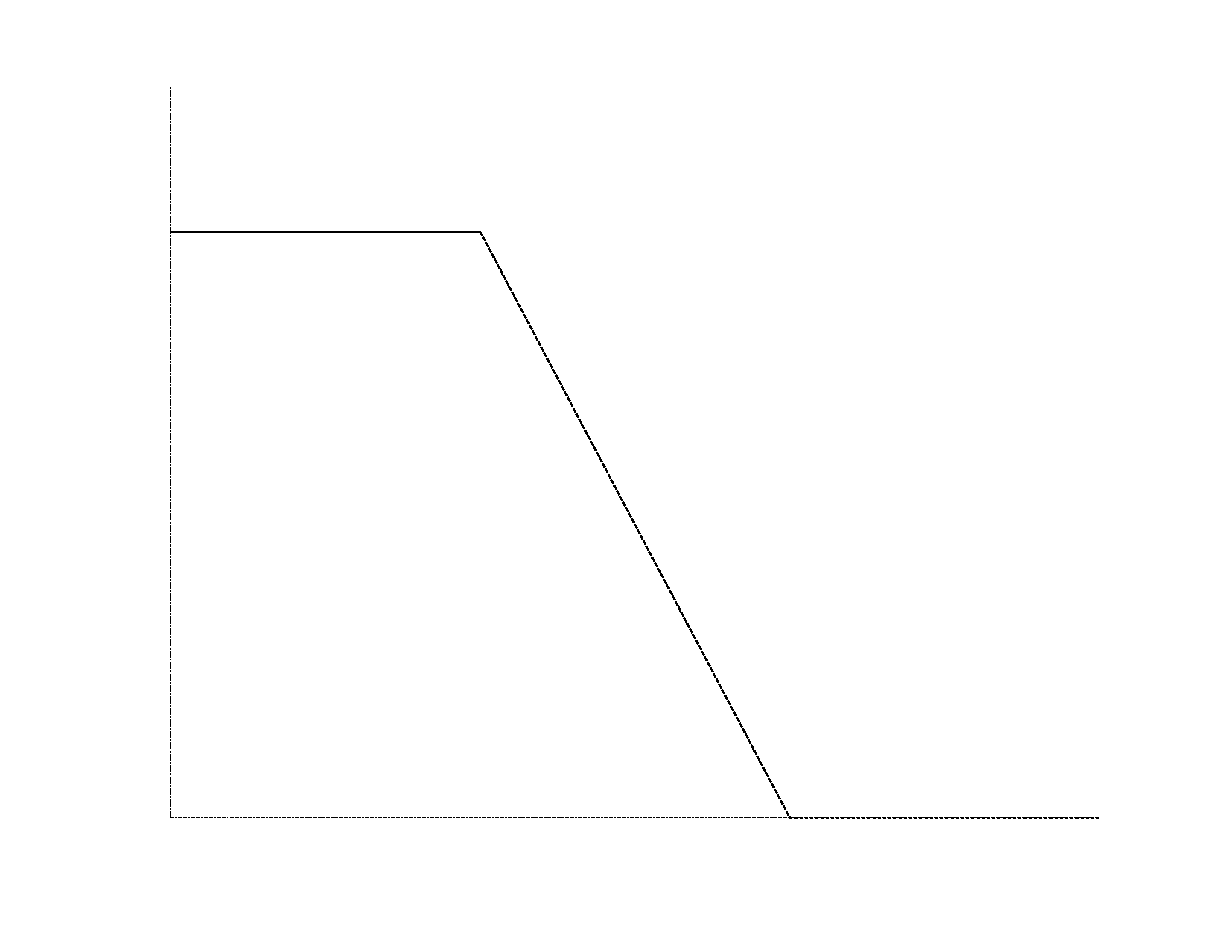
\includegraphics[scale=0.90]{highFreqResponseMosfetAmplifierBbodePlot}
\caption{ماسفیٹ ایمپلیفائر کا بوڈا خط}
\label{شکل_تعددی_ردعمل_ماسفیٹ_بوڈا_خط}
\end{figure}
%===============

\حصہ{مشترکہ کلکٹر  ایمپلیفائر کا بلند تعددی ردعمل}
شکل \حوالہ{شکل_تعددی_ردعمل_محاصل_مشترک} الف میں کلکٹر  مشترک ایمپلیفائر دکھایا گیا ہے جس کا مساوی باریک اشاراتی بلند تعددی دور شکل  ب میں دکھایا گیا ہے۔بلند تعدد پر بیرونی نسب کپیسٹر \عددی{C_b} قصر دور کردار ادا کرتا ہے۔شکل  ب سے واضح ہے کہ صرف \عددی{r_{b'e}} سے گزرتی برقی رو \عددی{i_b} کو ٹرانزسٹر \عددی{\beta} گنا بڑھاتا ہے۔اس شکل میں کپیسٹر \عددی{C_{b'e}} کا بائیں جانب کا مساوی تھونن دور حاصل کرتے ہیں
\begin{align*}
V_{th}&=\left(\frac{R_1 \mathbin{\|} R_2}{r_i+R_1 \mathbin{\|} R_2}\right) v_i =v_s\\
R_{th}&=r_i \mathbin{\|} R_1 \mathbin{\|} R_2 +r_{bb'}=r_s
\end{align*}
جہاں تھونن برقی دباو کو \عددی{v_s} اور تھونن برقی مزاحمت کو \عددی{r_s} لکھا گیا ہے۔شکل  ب میں \عددی{C_{b'c}} کا ایک سرا برقی زمین سے جڑا ہے۔یوں شکل  ب کو شکل \حوالہ{شکل_تعددی_ردعمل_محاصل_مشترک_سادہ_مساوی} کے طرز پر بنایا جا سکتا ہے۔
%  
\begin{figure}
\centering
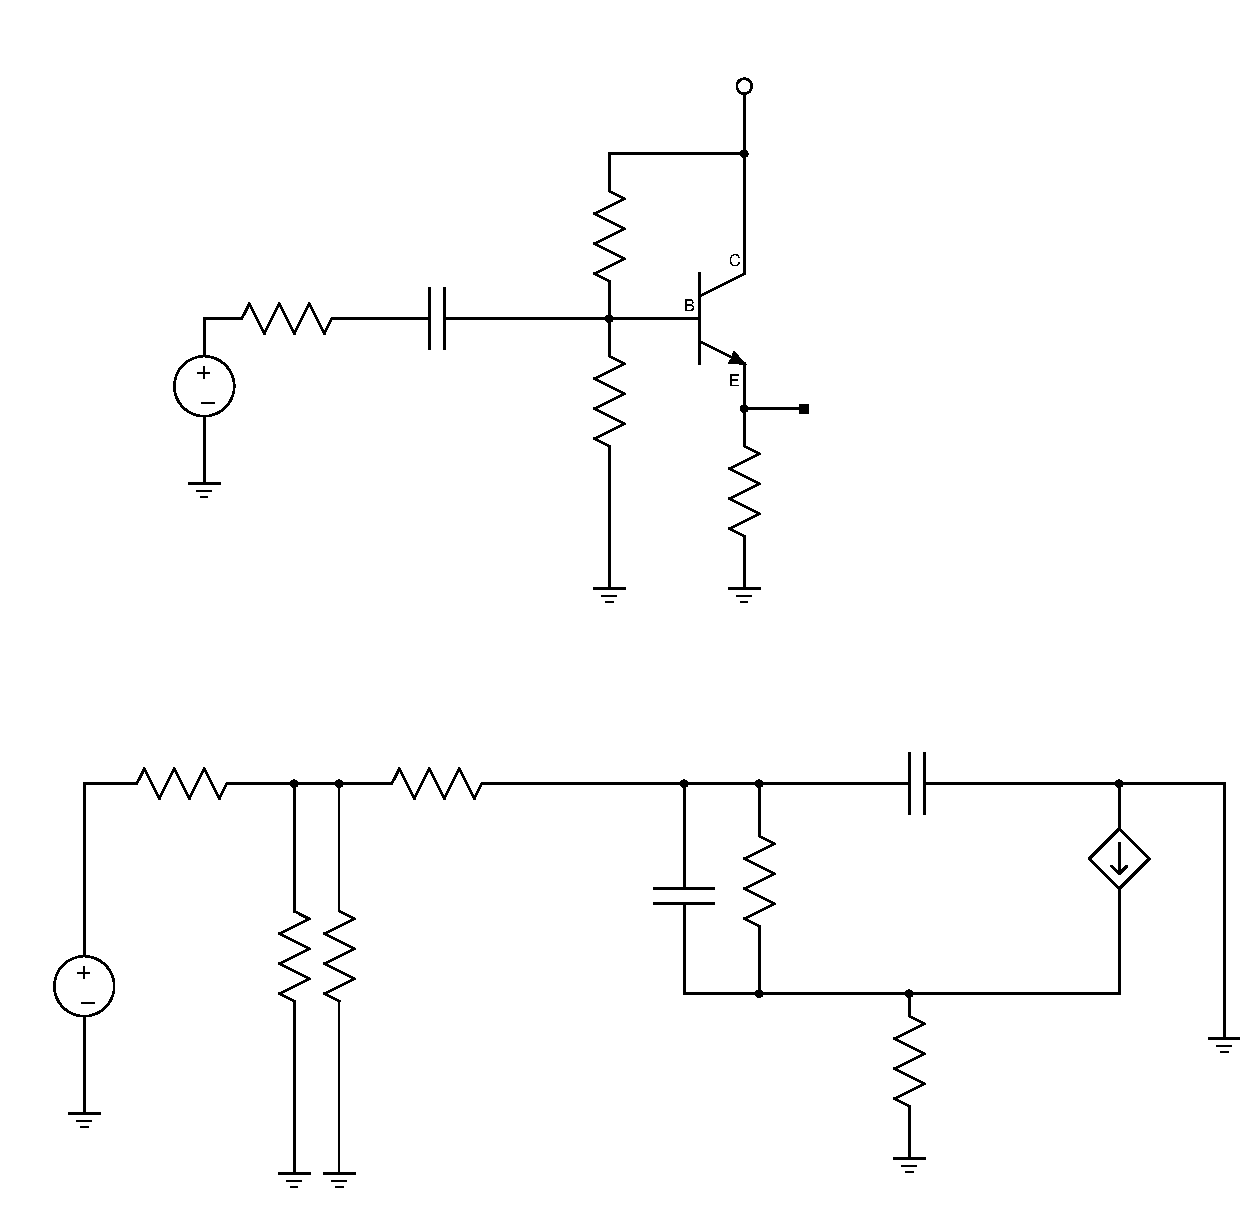
\includegraphics[scale=0.90]{commonCollectorHighFrequency}
\caption{کلکٹر  مشترک بلند تعددی رد عمل}
\label{شکل_تعددی_ردعمل_محاصل_مشترک}
\end{figure}
%
\begin{figure}
\centering
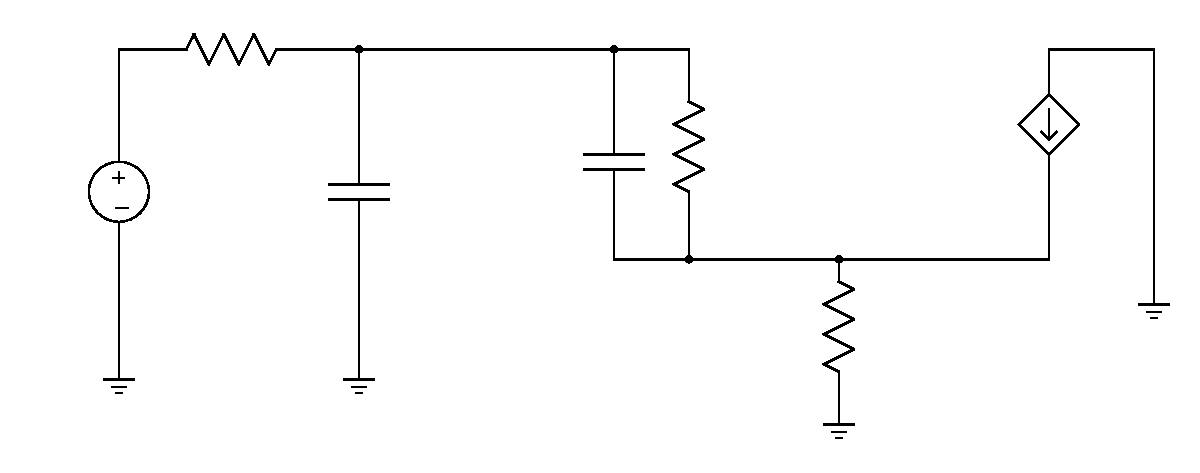
\includegraphics[scale=0.90]{commonCollectorHighFrequencyEquivalent}
\caption{کلکٹر  مشترک بلند تعددی سادہ مساوی دور}
\label{شکل_تعددی_ردعمل_محاصل_مشترک_سادہ_مساوی}
\end{figure}
اس شکل کو دیکھتے ہوئے کرخوف کے قانون برائے برقی رو کے استعمال سے ایمٹر        پر ہم لکھ سکتے ہیں
\begin{align*}
\left(v_e-v_1 \right)s C_{b'e} +\frac{v_e-v_1}{r_{b'e}} +\frac{v_e}{R_e}=\beta i_b=\beta \frac{v_1 -v_e}{r_{b'e}}
\end{align*}
یعنی
\begin{gather}
\begin{aligned}\label{مساوات_تعددی_ردعمل_مشترکہ_محاصل_سادہ_الف}
v_1&=\left[\frac{sC_{b'e}+\frac{\beta+1}{r_{b'e}}+\frac{1}{R_e}}{sC_{b'e}+\frac{\beta+1}{r_{b'e}}}\right] v_e\\
&=\left[\frac{\left(sC_{b'e}+\frac{\beta+1}{r_{b'e}}\right)+\frac{1}{R_e}}{sC_{b'e}+\frac{\beta+1}{r_{b'e}}}\right] v_e\\
&=\left[\frac{\left(sC_{b'e}+\frac{\beta+1}{r_{b'e}}\right)}{sC_{b'e}+\frac{\beta+1}{r_{b'e}}}+\frac{\frac{1}{R_e}}{sC_{b'e}+\frac{\beta+1}{r_{b'e}}}\right] v_e\\
&=\left[1+\frac{1}{R_e \left(sC_{b'e}+\frac{\beta+1}{r_{b'e}}\right)}\right] v_e
\end{aligned}
\end{gather}
اسی طرح جوڑ \عددی{v_1} پر کرخوف کے قانون برائے برقی رو کے استعمال سے ہم لکھ سکتے ہیں
\begin{align*}
\frac{v_1-v_s}{r_s}+v_1 sC_{b'c} +\left(v_1-v_e\right) sC_{b'e}+\frac{v_1-v_e}{r_{b'e}}=0
\end{align*}
یعنی
\begin{align*}
&\left(\frac{1}{r_s}+sC_{b'c}+sC_{b'e}+\frac{1}{r_{b'e}} \right) v_1=\frac{v_s}{r_s}+v_e \left(sC_{b'e}+\frac{1}{r_{b'e}} \right)\\
&\left(\frac{1}{r_s}+sC_{b'c}+sC_{b'e}+\frac{1}{r_{b'e}} \right) \left[1+\frac{1}{R_e \left(sC_{b'e}+\frac{\beta+1}{r_{b'e}}\right)}\right] v_e\\
&\hspace{6cm}\qquad{}=\frac{v_s}{r_s}+v_e \left(sC_{b'e}+\frac{1}{r_{b'e}} \right)
\end{align*}
جہاں دوسرے قدم پر مساوات \حوالہ{مساوات_تعددی_ردعمل_مشترکہ_محاصل_سادہ_الف} کا استعمال کیا گیا۔بائیں ہاتھ کے قوسین کو کھولتے ہیں
\begin{align*}
\left(\frac{1}{r_s}+sC_{b'c}+sC_{b'e}+\frac{1}{r_{b'e}} \right) v_e +\left[\frac{\frac{1}{r_s}+sC_{b'c}+sC_{b'e}+\frac{1}{r_{b'e}}}{R_e \left(sC_{b'e}+\frac{\beta+1}{r_{b'e}} \right)}\right] v_e\\
\hspace{6cm} =\frac{v_s}{r_s}+v_e \left(sC_{b'e}+\frac{1}{r_{b'e}} \right)
\end{align*}
اور یکساں اجزاء اکٹھے کرتے ہیں۔
\begin{align*}
\left[\frac{1}{r_s}+sC_{b'c}+\frac{\frac{1}{r_s}+sC_{b'c}+sC_{b'e}+\frac{1}{r_{b'e}}}{R_e \left(sC_{b'e}+\frac{\beta+1}{r_{b'e}} \right)}\right] v_e=\frac{v_s}{r_s}
\end{align*}
اس مساوات کو
\begin{align*}
\left[\frac{1}{r_s}\left(1+s r_s C_{b'c}\right)+\frac{\frac{1}{r_s}\left(1+s r_s C_{b'c}\right)+\frac{1}{r_{b'e}}\left(s r_{b'e}C_{b'e}+1\right)}{\frac{R_e\left(\beta+1 \right)}{r_{b'e}} \left(s \frac{r_{b'e}C_{b'e}}{\beta+1}+1 \right)}\right] v_e=\frac{v_s}{r_s}
\end{align*}
لکھ کر دونوں جانب کو \عددی{r_s} سے ضرب دیتے اور 
\begin{align}
\omega_1&=\frac{1}{r_s C_{b'c}}\\
\omega_{\beta}&=\frac{1}{r_{b'e} C_{b'e}}\\
\omega_T&=\frac{\beta+1}{r_{b'e}C_{b'e}}
\end{align}
لکھتے ہوئے یوں
\begin{align*}
\left[\left(1+\frac{j \omega}{\omega_1}\right)+\frac{\left(1+\frac{j \omega}{\omega_1}\right)+\frac{r_s}{r_{b'e}}\left(\frac{j \omega}{\omega_{\beta}}+1\right)}{\frac{R_e\left(\beta+1 \right)}{r_{b'e}} \left(\frac{j \omega}{\omega_T}+1 \right)}\right] v_e=v_s
\end{align*}
یا
\begin{align*}
\left[\frac{\frac{R_e\left(\beta+1 \right)}{r_{b'e}} \left(\frac{j \omega}{\omega_T}+1 \right)\left(1+\frac{j \omega}{\omega_1}\right)+\left(1+\frac{j \omega}{\omega_1}\right)+\frac{r_s}{r_{b'e}}\left(\frac{j \omega}{\omega_{\beta}}+1\right)}{\frac{R_e\left(\beta+1 \right)}{r_{b'e}} \left(\frac{j \omega}{\omega_T}+1 \right)}\right] v_e=v_s
\end{align*}
لکھا جا سکتا ہے۔کسر کے بالائی حصے میں تمام قوسین کھولتے ہوئے اس مساوات کو یوں لکھا جا سکتا ہے
\begin{align*}
\frac{A+j \omega B +\left(j \omega \right)^2  C}{\frac{R_e\left(\beta+1 \right)}{r_{b'e}} \left(\frac{j \omega}{\omega_T}+1 \right)}=\frac{v_s}{v_e}
\end{align*}
جہاں
\begin{align*}
A&=\frac{R_e\left(\beta+1 \right)}{r_{b'e}}+1+\frac{r_s}{r_{b'e}}\\
B&=\frac{R_e\left(\beta+1 \right)}{r_{b'e} \omega_T} +\frac{R_e\left(\beta+1 \right)}{r_{b'e}\omega_1}+\frac{1}{\omega_1}+\frac{r_s}{r_{b'e}\omega_{\beta}}\\
C&=\frac{R_e\left(\beta+1 \right)}{r_{b'e} \omega_T \omega_1}
\end{align*}
کے برابر ہیں۔اس سے
\begin{align}
\frac{v_e}{v_s}=\frac{\frac{R_e\left(\beta+1 \right)}{r_{b'e}} \left(\frac{j \omega}{\omega_T}+1 \right)}{A+j \omega B +\left(j \omega \right)^2  C}
\end{align}
حاصل ہوتا ہے۔اگر \عددی{\left( \beta +1\right) R_e \gg r_s +r_{b'e}}  ہو تب اس مساوات کو اس طرح لکھا جا سکتا ہے
\begin{align}
\frac{v_e}{v_s}=\frac{1+\frac{j \omega}{\omega_T}}{1+j \omega \left(\frac{1}{\omega_1}+\frac{1+\frac{r_s}{R_e}}{\omega_T} \right)+\frac{j \omega}{\omega_T}\frac{j \omega}{\omega_1}}
\end{align}
%=============
\حصہ{مشترک بیس  ایمپلیفائر کا بلند انقطاعی تعدد}
شکل \حوالہ{شکل_تعددی_ردعمل_قابو_مشترک_ایمپلیفائر_بلند_تعدد_پر} میں بیس  مشترک ایمپلیفائر دکھایا گیا ہے۔صفحہ \حوالہصفحہ{شکل_ٹی_ماڈل} پر ٹرانزسٹر کا \اصطلاح{ٹی ریاضی نمونہ} دکھایا گیا ہے جسے \اصطلاح{پائے ریاضی نمونہ} کی شکل میں بناتے ہوئے شکل \حوالہ{شکل_تعددی_ردعمل_قابو_مشترک_ایمپلیفائر_بلند_تعدد_پر} کا بلند تعددی مساوی دور شکل \حوالہ{شکل_تعددی_ردعمل_قابو_مشترک_ایمپلیفائر_بلند_تعدد_پر_مساوی} میں دکھایا گیا ہے۔باریک اشاراتی دور میں \عددی{R_1} اور \عددی{R_2} دونوں کے دونوں سرے برقی زمین پر ہیں لہٰذا انہیں نہیں دکھایا گیا۔چونکہ ٹرانزسٹر کا بیس  سرا برقی زمین پر ہے لہٰذا \عددی{C_{b'c}} کا ایک سرا برقی زمین پر ہو گا اور یوں اسے کلکٹر  اور برقی زمین کے مابین دکھایا گیا ہے۔ 

\begin{figure}
\centering
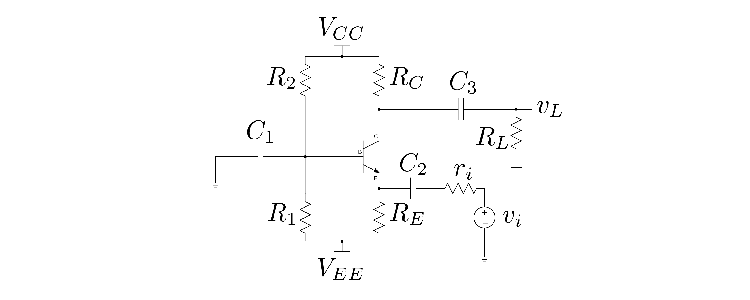
\includegraphics[scale=0.90]{commonBaseFrequencyResponseAtHighFrequency}
\caption{بیس  مشترک ایمپلیفائر}
\label{شکل_تعددی_ردعمل_قابو_مشترک_ایمپلیفائر_بلند_تعدد_پر}
\end{figure}
%
\begin{figure}
\centering
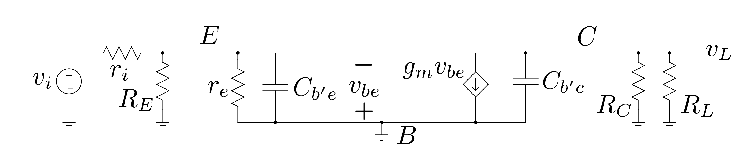
\includegraphics[scale=0.90]{commonBaseFrequencyResponseAtHighFrequencyEquivalent}
\caption{بیس  مشترک ایمپلیفائر کا مساوی دور}
\label{شکل_تعددی_ردعمل_قابو_مشترک_ایمپلیفائر_بلند_تعدد_پر_مساوی}
\end{figure}

مساوی دور سے دو انقطاعی تعدد حاصل ہوتے ہیں یعنی 
%
\begin{gather}
\begin{aligned}\label{مساوات_تعددی_ردعمل_مشترک_قابو_بلند_کونے_کے_تعدد}
\omega_{H1}&=\frac{1}{\left(r_e \mathbin{\|} R_E \mathbin{\|} r_i \right) C_{b'e} }\\
\omega_{H2}&=\frac{1}{\left(R_C \mathbin{\|} R_L \right) C_{b'c}}
\end{aligned}
\end{gather}
درمیانی تعدد پر افزائش حاصل کرتے وقت \عددی{C_{b'c}} اور \عددی{C_{b'e}} کو کھلے دور تصور کیا جاتا ہے۔یوں
\begin{align*}
A_v=\frac{v_L}{v_i}&=\frac{v_L}{ i_c} \times \frac{i_c}{v_{b'e}} \times \frac{v_{b'e}}{v_i}\\
&=-\left(R_C \mathbin{\|} R_L\right) g_m \left(-\frac{R_E \mathbin{\|} r_e}{R_E \mathbin{\|} r_e+r_i} \right)\\
&=\left(R_C \mathbin{\|} R_L\right) g_m \left(\frac{R_E \mathbin{\|} r_e}{R_E \mathbin{\|} r_e+r_i} \right)
\end{align*}
لکھا جا سکتا ہے جہاں پہلی اور تیسری قوسین  میں موجود منفی ایک آپس میں ضرب ہو کر ختم ہو جاتے ہیں۔
%=============
\ابتدا{مثال}
شکل \حوالہ{شکل_تعددی_ردعمل_قابو_مشترک_ایمپلیفائر_بلند_تعدد_پر} میں
\begin{align*}
V_{CC}&=\SI{5}{\volt}, \hspace{5mm} V_{EE}=\SI{-5}{\volt}, \hspace{5mm} R_{E}=\SI{600}{\ohm}\\
R_1&=\SI{6}{\kilo \ohm} \hspace{5mm} R_2=\SI{38}{\kilo \ohm}, \hspace{5mm} R_C=\SI{5}{\kilo \ohm}\\
R_L&=\SI{10}{\kilo \ohm}, \hspace{5mm} r_i=\SI{100}{\ohm}
\end{align*}
ہیں۔ٹرانزسٹر کا \عددی{\beta=149}، \عددی{C_{b'e}=\SI{35}{\pico \farad}} اور \عددی{C_{b'c}=\SI{4}{\pico \farad}} ہیں۔بلند کونے کے تعدد حاصل کریں۔

حل:پہلے یک سمتی  حل درکار ہے۔تھونن مساوی اجزاء حاصل  کرتے ہیں۔
\begin{align*}
V_{BB}&=\frac{5+5}{6000+38000} \times 6000-5=\SI{-3.64}{\volt}\\
R_B&=\frac{6000 \times 38000}{6000 +38000}=\SI{5.182}{\kilo \ohm}
\end{align*}
یوں
\begin{align*}
I_E=\frac{-3.64-0.7+5}{\frac{5182}{149+1}+600}=\SI{1.04}{\milli \ampere}
\end{align*}
یوں
\begin{align*}
g_m&=\frac{1.04 \times 10^{-3}}{25 \times 10^{-3}}=\SI{0.0416}{\siemens}\\
r_e&=\SI{24}{\ohm}\\
r_{b'e}&=24 \times 150=\SI{3.6}{\kilo \ohm}
\end{align*}
حاصل ہوتے ہیں۔

\عددی{C_{b'e}} کے متوازی کل مزاحمت \عددی{R_{b'e}}
\begin{align*}
\frac{1}{R_{be'}}&=\frac{1}{24}+\frac{1}{600}+\frac{1}{100}\\
R_{b'e}&=\SI{18.75}{\ohm}
\end{align*}
جبکہ \عددی{C_{b'c}} کے متوازی کل مزاحمت
\begin{align*}
R_{b'c}=\frac{5000 \times 10000}{5000+10000}=\SI{3.333}{\kilo \ohm}
\end{align*}
ہیں۔یوں مساوات \حوالہ{مساوات_تعددی_ردعمل_مشترک_قابو_بلند_کونے_کے_تعدد} کی مدد سے
\begin{align*}
f_{H1}&=\frac{1}{2 \times \pi \times 18.75 \times 35 \times 10^{-12}}=\SI{242}{\mega \hertz}\\
f_{H2}&=\frac{1}{2 \times \pi \times 3333 \times 4 \times 10^{-12}}=\SI{11.93}{\mega \hertz}
\end{align*}
حاصل ہوتے ہیں لہٰذا اس ایمپلیفائر کا بلند انقطاعی تعدد \عددی{\SI{11.93}{\mega \hertz}} ہے۔اس مثال میں بلند انقطاعی تعدد کا دارومدار \عددی{C_{b'c}}  پر ہے نا کہ \عددی{C_{b'e}} پر۔
\begin{align*}
A_v&=\left(\frac{5000 \times 10000}{5000+1000}\right) 0.0416 \left(\frac{\frac{24 \times 600}{24+600}}{\frac{24 \times 600}{24+600} +100} \right)\\
&=\SI{26}{\volt \per \volt}
\end{align*}
\انتہا{مثال}
%==================
\ابتدا{مثال}
گزشتہ مثال کے دور میں اگر داخلی اشارہ بیس  پر مہیا کیا جائے تو ایمٹر        مشترک ایمپلیفائر حاصل ہوتا ہے جسے شکل \حوالہ{شکل_تعددی_ردعمل_مخارج_مشترک_ایمپلیفائر_اور_قابو_مشترک_موازنہ} میں دکھایا گیا ہے۔بقایا تمام متغیرات وہی رکھتے ہوئے دیکھتے ہیں کہ اس صورت میں بلند انقطاعی تعدد کیا حاصل ہوتا ہے۔

\begin{figure}
\centering
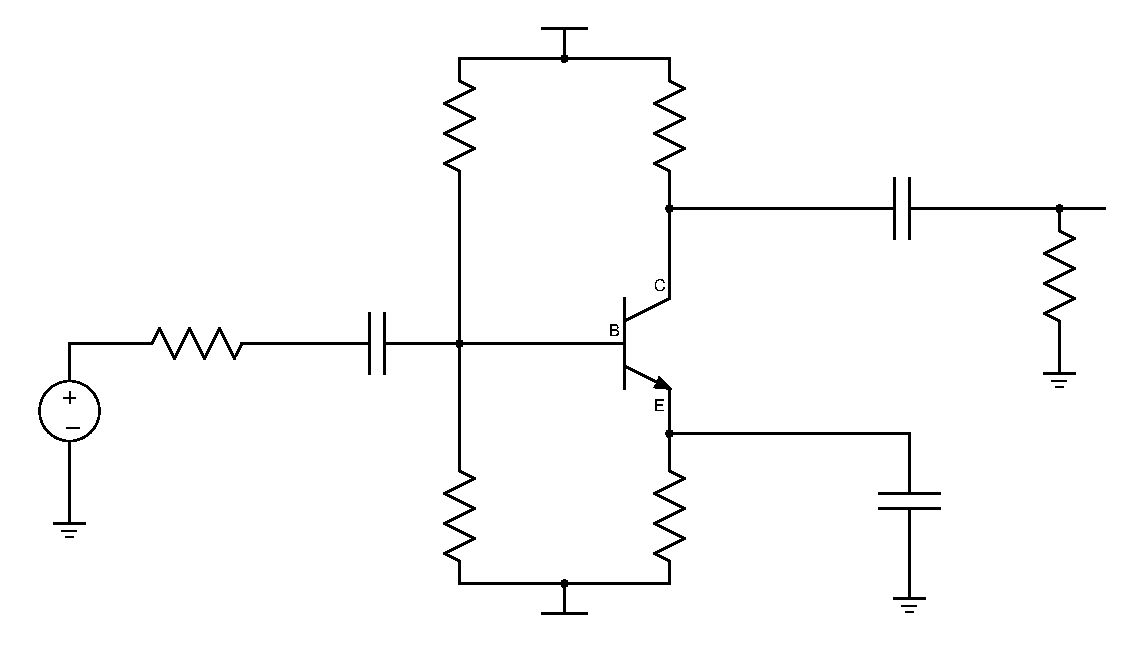
\includegraphics[scale=0.90]{commonEmitterFrequencyResponseAtHighFrequencyComparingToCommonBase}
\caption{ایمٹر        مشترک ایمپلیفائر}
\label{شکل_تعددی_ردعمل_مخارج_مشترک_ایمپلیفائر_اور_قابو_مشترک_موازنہ}
\end{figure}

حل:مساوی دور شکل \حوالہ{شکل_تعددی_ردعمل_مخارج_مشترک_ایمپلیفائر_اور_قابو_مشترک_موازنہ_مساوی} میں دکھایا گیا ہے۔گزشتہ مثال کی معلومات استعمال کرتے ہوئے
\begin{align*}
&C_M=\left(1+0.0416 \times  3333\right) \times 4 \times 10^{-12}=\SI{559}{\pico \farad}\\
&C_{b'e}+C_M=\SI{594}{\pico \farad}
\end{align*}
اور اس کے متوازی کل مزاحمت \عددی{R_m}
\begin{align*}
\frac{1}{R_m}&=\frac{1}{100}+\frac{1}{5182}+\frac{1}{3600}\\
R_m&=\SI{95.5}{\ohm}
\end{align*}
حاصل ہوتا ہے۔یوں بلند انقطاعی تعدد
\begin{align*}
f_H=\frac{1}{2 \pi \times 95.5 \times 594 \times 10^{-12}}=\SI{2.8}{\mega \hertz}
\end{align*}
اور درمیانی تعدد پر افزائش
\begin{align*}
A_v=\frac{v_L}{v_i}&=-3333 \times 0.0416 \times \frac{\frac{3600 \times 5182}{3600+5182}}{\frac{3600 \times 5182}{3600+5182}+100} 
=\SI{-132}{\volt \per \volt}
\end{align*}
%
\begin{figure}
\centering
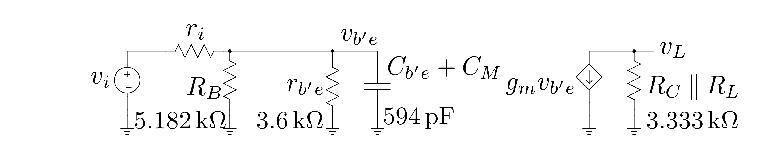
\includegraphics[scale=0.90]{commonEmitterFrequencyResponseAtHighFrequencyComparingToCommonBaseEquivalent}
\caption{ایمٹر        مشترک ایمپلیفائر کے انقطاعی تعدد حاصل کرنے کے لئے درکار مساوی دور}
\label{شکل_تعددی_ردعمل_مخارج_مشترک_ایمپلیفائر_اور_قابو_مشترک_موازنہ_مساوی}
\end{figure}
%

مندرجہ بالا دو مساوات سے آپ دیکھ سکتے ہیں کہ بیس  مشترک ایمپلیفائر کی بلند انقطاعی تعدد ایمٹر        مشترک ایمپلیفائر کے بلند انقطاعی تعدد سے تقریباً سوا چار گنا زیادہ ہے۔
\انتہا{مثال}
%==========
\حصہ{کیسکوڈ ایمپلیفائر}
ایمپلیفائر کے \اصطلاح{بلند تعددی} رد عمل پر غور کے دوران یہ حقیقت سامنے آئی کہ اگرچہ \عددی{C_{b'c}} کی قیمت نہایت کم لیکن \اصطلاح{ملر کپیسٹر}\فرہنگ{ملر کپیسٹر}\فرہنگ{Miller capacitor}\حاشیہب{Miller capacitor} کی وجہ سے بلند انقطاعی نقطہ تعین کرنے میں اس کا کردار نہایت اہم ہے۔ٹرانزسٹر ایمپلیفائر بلند انقطاعی نقطے سے کم تعدد کے اشارات کو بڑھاتا ہے۔یوں ہم چاہیں گے کہ یہ نقطہ بلند سے بلند تر تعدد پر پایا جائے۔اس حصے میں \اصطلاح{کیسکوڈ ایمپلیفائر}\فرہنگ{کیسکوڈ}\فرہنگ{cascode amplifier}\حاشیہد{فریڈرک ونٹن ہنٹ نے اس ایمپلیفائر کو دریافت کیا اور اس کا نام کیسکوڈ ایمپلیفائر رکھا۔} پر غور کیا جائے گا جس میں ملر کپیسٹر کی قیمت کم سے کم ہونے کی بنا پر زیادہ سے زیادہ تعدد پر بلند تر انقطاعی نقطہ حاصل ہوتا ہے۔\حاشیہب{cascode amplifier}

شکل \حوالہ{شکل_تعددی_ردعمل_کیسکوڈ_ایمپلیفائر} الف میں کیسکوڈ ایمپلیفائر دکھایا گیا ہے۔\عددی{Q_1} اور اس کے ساتھ منسلک \عددیء{R_1}، \عددیء{R_2}، \عددی{R_E} اور  \عددی{C_E}  مل کر مشترکہ ایمٹر        طرز کا ایمپلیفائر بناتے ہیں جسے کپیسٹر \عددی{C_{B1}} کے ذریعہ داخلی اشارہ \عددی{v_i} فراہم کیا گیا ہے۔\عددی{R_i} داخلی اشارہ فراہم کرنے والے کی مزاحمت ہے۔عام صورت میں \عددی{Q_1} کے کلکٹر  پر برقی بوجھ \عددی{R_L} لادا جاتا ہے لیکن کیسکوڈ میں ایسا نہیں کیا جاتا۔کیسکوڈ میں \عددی{Q_2} بطور برقی بوجھ کردار ادا کرتا ہے۔ \عددی{Q_2} کے بیس  پر بیرونی کپیسٹر \عددی{C_{B2}} کا کردار نہایت اہم ہے۔درکار تعدد پر  \عددی{C_{B2}} بطور قصر دور کام کرتے ہوئے \عددی{Q_2} کے بیس  کو برقی زمین پر رکھتا ہے۔\عددی{Q_2} اور اس کے ساتھ منسلک \عددیء{R_1'}، \عددی{R_2'} اور \عددی{C_{B2}} مل کر مشترکہ بیس  طرز کا ایمپلیفائر بناتے ہیں۔

کیسکوڈ کی بلند انقطاعی تعدد اس میں پائے جانے والے \عددی{Q_1}  پر مبنی مشترکہ ایمٹر طرز کے ایمپلیفائر اور \عددی{Q_2} پر مبنی مشترکہ بیس  طرز کے ایمپلیفائر  کی بلند انقطاعی تعدد پر منحصر ہو گی۔مساوات \حوالہ{مساوات_تعددی_ردعمل_بلند_انقطاعی_بیٹا_تعدد} اور مساوات \حوالہ{مساوات_تعددی_ردعمل_مشترکہ_قابو_بلند_انقطاعی_نکتہ} ان ایمپلیفائر کی قصر دور بلند تر انقطاعی تعدد \عددی{\omega_{\beta}} اور \عددی{\omega_{\alpha}} دیتے ہیں جن کے تحت \عددی{\omega_{\alpha}=\beta \omega_{\beta}=\omega_T} کے برابر ہے جہاں \عددی{\omega_{\beta}} مشترکہ ایمٹر  طرز کے ایمپلیفائر کی قصر دور بلند انقطاعی تعدد جبکہ \عددی{\omega_{\alpha}} مشترکہ بیس  طرز کے ایمپلیفائر کی قصر دور بلند انقطاعی تعدد ہے۔چونکہ \عددی{\omega_{\alpha}=\omega_T} کے برابر ہے لہٰذا مشترکہ بیس  طرز کا ایمپلیفائر ٹرانزسٹر کے \عددی{\omega_T} تعدد تک قابل استعمال ہوتا ہے۔اس کے برعکس مشترکہ ایمٹر طرز کے ایمپلیفائر کی بلند انقطاعی تعدد \عددی{C_M} پر منحصر ہوتی ہے جو از خود اس پر لدے برقی بوجھ \عددی{R_L} پر منحصر ہوتا ہے۔یوں کیسکوڈ ایمپلیفائر کی بلند تعددی انقطاعی تعدد اس میں پائے جانے والے مشترکہ ایمٹر ایمپلیفائر کی بلند انقطاعی تعدد پر منحصر ہو گا۔آئیں اب اس پر غور کریں۔
\begin{figure}
\centering
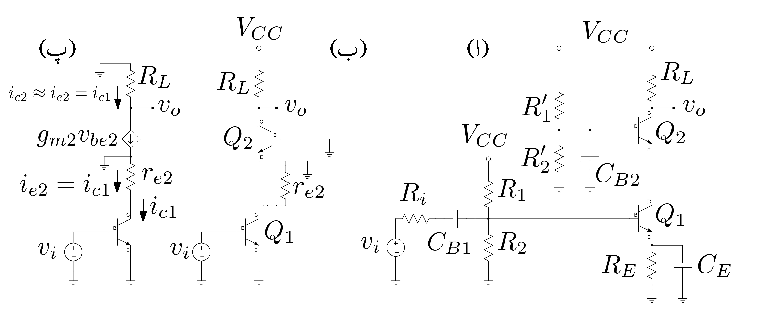
\includegraphics[scale=0.90]{cascodeAmplifierA}
\caption{کیسکوڈ ایمپلیفائر}
\label{شکل_تعددی_ردعمل_کیسکوڈ_ایمپلیفائر}
\end{figure}

شکل \حوالہ{شکل_تعددی_ردعمل_کیسکوڈ_ایمپلیفائر} ب میں کیسکوڈ ایمپلیفائر کا مساوی باریک اشاراتی دور دکھایا گیا ہے جس میں ٹرانزسٹر مائل کرنے والے اجزاء  نہیں دکھائے گئے تا کہ کیسکوڈ ایمپلیفائر کی بنیادی کارکردگی پر توجہ رہے۔اس شکل میں \عددی{Q_2} کا مزاحمت \عددی{r_{e2}} بطور \عددی{Q_1} کے برقی بوجھ  کردار ادا کرتا ہے۔\عددی{r_{e2}} کو \عددی{Q_2} کے باہر دکھاتے ہوئے اسے \عددی{Q_1} کے کلکٹر  اور برقی زمین کے مابین دکھایا گیا ہے۔شکل  پ میں \عددی{Q_2} کا \عددیء{T} ریاضی نمومے\حاشیہد{\عددی{T} ریاضی نمونے پر حصہ \حوالہ{حصہ_ٹرانزسٹر_ٹی_ماڈل} میں تبصرہ کیا گیا ہے} استعمال کرتے ہوئے اس بات کی وضاحت کی گئی ہے کہ \عددی{Q_1} کے کلکٹر  اور برقی زمین کے درمیان \عددی{r_{e2}} نسب ہے۔

\عددی{Q_1} کا برقی بوجھ \عددی{r_{e2}} لیتے ہوئے
\begin{align}
C_M=\left(1+g_{m1} r_{e2} \right) C_{b'c}
\end{align}
حاصل ہوتا ہے۔چونکہ \عددی{Q_1} اور \عددی{Q_2} میں برابر یک سمتی برقی رو \عددی{I_{CQ}} گزرتا ہے لہٰذا \عددی{g_{m1}=g_{m2}=g_m=\frac{I_{CQ}}{V_T}} اور \عددی{r_{e1}=r_{e2}=\frac{1}{g_m}=r_e} ہوں گے۔آپ یہ بھی دیکھ سکتے ہیں کہ باریک اشاراتی برقی رو \عددی{i_{c1}=i_{e2} \approx i_{c2}} ہو گا۔یوں  \عددی{g_{m1} r_{e2} =1} لیتے ہوئے
\begin{align}
C_M=\left(1+1 \right) C_{b'c}=2 C_{b'c}
\end{align}
حاصل ہوتا ہے جو کہ کم ترین ممکنہ ملر کپیسٹر ہے۔\عددی{C_M} کی قیمت کم سے کم ہونے کی بنا پر مشترکہ ایمٹر        طرز کے ایمپلیفائر کی  بلند انقطاعی تعدد زیادہ سے زیادہ تعدد پر حاصل ہوتی ہے۔

شکل \حوالہ{شکل_تعددی_ردعمل_کیسکوڈ_ایمپلیفائر_باریک_اشاراتی_تجزیہ} میں \عددی{Q_1} کا بلند تعددی ریاضی نمونہ استعمال کرتے  ہوئے باریک اشاراتی مساوی دور دکھایا گیا ہے جس میں \عددی{r_{e2}} کو بطور برقی بوجھ دکھایا گیا ہے۔متوازی جڑے \عددی{R_1} اور \عددی{R_2} کے کل مزاحمت کو \عددی{R_B} لکھتے  ہیں یعنی
\begin{align*}
\frac{1}{R_B}=\frac{1}{R_1}+\frac{1}{R_2}
\end{align*}
یوں متوازی جڑے مزاحمت \عددیء{R_1}، \عددی{R_2} اور \عددی{r_{be}} کی کل مقدار \عددی{R_m} یوں لکھی جا سکتی ہے۔
\begin{align*}
\frac{1}{R_m}&=\frac{1}{R_1}+\frac{1}{R_2}+\frac{1}{r_{be}}\\
&=\frac{1}{R_B}+\frac{1}{r_{be}}
\end{align*}
یعنی
\begin{align*}
R_m=\frac{R_B r_{be}}{R_B+r_{be}}
\end{align*}
اسی طرح متوازی جڑے \عددی{R_m} اور دو کپیسٹروں کی برقی رکاوٹ \عددی{Z} کو یوں لکھ سکتے ہیں۔
\begin{align*}
\frac{1}{Z}&=j \omega \left( C_{b'e}+2 C_{b'c} \right)+\frac{1}{R_m}
\end{align*}
 ایمپلیفائر کی موصل نما افزائش \عددی{G_M=\frac{i_c}{v_i}} یوں حاصل ہوتی ہے۔
\begin{align*}
G_m&=\frac{i_{c1}}{v_i}=\left(\frac{i_c}{v_{be}} \right) \left(\frac{v_{be}}{v_i} \right)\\
&=g_m \left(\frac{Z}{R_i+Z} \right)\\
&=g_m \left[\frac{Z}{Z\left( \frac{R_i}{Z}+1\right)} \right]\\
&=\frac{g_m}{ \frac{R_i}{Z}+1}
\end{align*}
اس میں \عددی{\frac{1}{Z}} استعمال کرتے 
\begin{align*}
G_m &= \frac{g_m}{ R_i \left[j \omega \left( C_{b'e}+2 C_{b'c} \right) +\frac{1}{R_m} \right]+1}\\
&=\frac{g_m}{ j \omega \left( C_{b'e}+2 C_{b'c} \right) R_i+\frac{R_i}{R_m} +1}
\end{align*}
حاصل ہوتا ہے۔اس کے نچلے  حصے سے \عددی{\left(\frac{R_i}{R_m}+1 \right)} باہر لیتے ہوئے
\begin{align*}
G_m &=\frac{g_m}{ \left(\frac{R_i}{R_m}+1 \right) \left[j \omega \frac{\left( C_{b'e}+2 C_{b'c} \right)  R_i}{\frac{R_i}{R_m}+1}+1 \right]}
\end{align*}
حاصل ہوتا ہے جس میں
\begin{align}
\omega_H= \frac{\frac{R_i}{R_m}+1}{\left( C_{b'e}+2 C_{b'c} \right)  R_i}
\end{align}
لکھتے ہوئے
\begin{align}
G_m &=\left(\frac{g_m}{\frac{R_i}{R_m}+1} \right) \left(\frac{1}{j \frac{\omega}{\omega_H} +1}\right)
\end{align}
حاصل ہوتا ہے۔
\begin{figure}
\centering
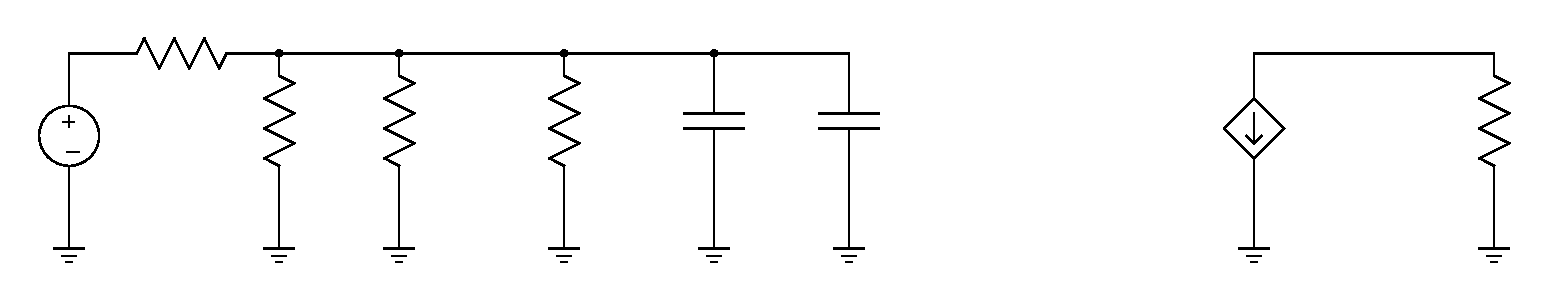
\includegraphics[scale=0.90]{cascodeAmplifierB}
\caption{کیسکوڈ ایمپلیفائر باریک اشاراتی تجزیہ}
\label{شکل_تعددی_ردعمل_کیسکوڈ_ایمپلیفائر_باریک_اشاراتی_تجزیہ}
\end{figure}

شکل \حوالہ{شکل_تعددی_ردعمل_کیسکوڈ_ایمپلیفائر} پ میں اس بات کی وضاحت کی گئی ہے کہ \عددی{Q_2} میں وہی برقی رو گزرتی ہے جو \عددی{Q_1} میں گزرتی ہے اور یوں \عددی{i_{c2} = i_{c1}} ہوتا ہے۔اس حقیقت کو مدِ نظر رکھتے ہوئے کیسکوڈ ایمپلیفائر کے برقی دباو کی افزائش 
\begin{align*}
A_v&=\frac{v_o}{v_i}=\left( \frac{v_o}{i_{c2}} \right) \left(\frac{i_{c2}}{i_{c1}} \right) \left(\frac{i_{c1}}{v_i} \right)\\
&=\left( \frac{v_o}{i_{c2}} \right) \left(\frac{i_{c2}}{i_{c1}} \right) \left(G_m \right)\\
&=\left(-R_L \right) \left(1 \right) \left(G_m \right)
\end{align*}
یعنی
\begin{gather}
\begin{aligned}
A_v&=-\left(\frac{g_m R_L}{\frac{R_i}{R_m}+1} \right) \left(\frac{1}{j \frac{\omega}{\omega_H} +1}\right)\\
&=A_{vD} \left(\frac{1}{j \frac{\omega}{\omega_H} +1}\right)
\end{aligned}
\end{gather}
حاصل ہوتی ہے جہاں \عددی{A_{vD}} درمیانی تعدد پر افزائش ہے جو
\begin{align}\label{مساوات_تعددی_ردعمل_کیسکوڈ_درمیانی_تعدد_کی_افزائش}
A_{vD}=-\left(\frac{g_m R_L}{\frac{R_i}{R_m}+1} \right) =-\left(\frac{g_m R_L R_m}{R_i+R_m}\right)
\end{align}
کے برابر ہے۔اس طرح کیسکوڈ ایمپلیفائر پوری برقی دباو کی افزائش دیتے ہوئے بلند انقطاعی تعدد کو بلند تر تعدد تک لی جاتا ہے۔\عددی{\omega_H} کو مزید
\begin{gather}
\begin{aligned}\label{مساوات_تعددی_ردعمل_کیسکوڈ_بلند_انقطاعی_تعدد}
\omega_H&= \frac{R_i+R_m}{\left( C_{b'e}+2 C_{b'c} \right)  R_i R_m}\\
&=\frac{1}{\left( C_{b'e}+2 C_{b'c} \right)  \frac{R_i R_m}{R_i+R_m}}
\end{aligned}
\end{gather}
لکھا جا سکتا ہے جہاں کپیسٹر \عددی{C_{b'e}+2C_{b'c}} کے متوازی کل مزاحمت \عددی{R_i \mathbin{\|} R_m}  دراصل متوازی جڑے \عددیء{R_i}، \عددیء{R_1}، \عددیء{R_2} اور \عددیء{r_{be}} کی کل مزاحمت ہے۔آپ دیکھ سکتے ہیں کہ کیسکوڈ ایمپلیفائر کی بلند انقطاعی تعدد کو بھی \عددی{\omega_H=\frac{1}{R C}} کی شکل میں لکھا جا سکتا ہے جہاں \عددی{C} کل کپیسٹر اور \عددی{R} اس کے ساتھ متوازی جڑی کل مزاحمت ہے۔

شکل \حوالہ{شکل_تعددی_ردعمل_کیسکوڈ_ایمپلیفائر} الف میں\عددی{Q_1} مشترک ایمٹر ایمپلیفائر ہے۔اگر \عددی{Q_2} کو دور سے نکال کر \عددی{R_L} کو \عددی{Q_1} کے کلکٹر کے ساتھ جوڑا جائے تو شکل \حوالہ{شکل_تعددی_ردعمل_کیسکوڈ_ایمپلیفائر_مشترک_مخارج_حصہ} میں دکھایا گیا مشترک ایمٹر ایمپلیفائر حاصل ہو گا جس کا درمیانی تعدد پر مساوی دور بھی اسی شکل میں دکھایا گیا ہے۔آئیں زنجیری ضرب کی مدد سے شکل \حوالہ{شکل_تعددی_ردعمل_کیسکوڈ_ایمپلیفائر_مشترک_مخارج_حصہ} کا \عددی{A_v=\tfrac{v_L}{v_i}} حاصل کریں۔
\begin{figure}
\centering
\includegraphics[scale=0.90]{cascodeCommonEmitterSection}
\caption{کیسکوڈ ایمپلیفائر کا مشترک ایمٹر حصہ}
\label{شکل_تعددی_ردعمل_کیسکوڈ_ایمپلیفائر_مشترک_مخارج_حصہ}
\end{figure}

\begin{gather}
\begin{aligned}
A_v=\frac{v_L}{v_i}&=\frac{v_L}{i_c} \times \frac{i_c}{v_{be1}} \times \frac{v_{be1}}{v_i}\\
&=-R_L g_{m} \left(\frac{R_m}{R_i+R_m}\right)\\
&=\frac{-g_m R_L R_i}{R_i +R_m}
\end{aligned}
\end{gather}
اس مساوات کا مساوات \حوالہ{مساوات_تعددی_ردعمل_کیسکوڈ_درمیانی_تعدد_کی_افزائش} کے ساتھ موازنہ کرنے سے ثابت ہوتا ہے کہ کیسکوڈ ایمپلیفائر کی درمیانی تعدد پر افزائش وہی ہے جو مشترک ایمٹر ایمپلیفائر کی ہے۔کیسکوڈ ایمپلیفائر کی افادیت اس حقیقت میں ہے کہ اس کا بلند انقطاعی تعدد کافی زیادہ تعدد پر پایا جاتا ہے۔
%=====================
\ابتدا{مثال}\شناخت{مثال_تعددی_ردعمل_کیسکوڈ_افزائش_انقطاعی_تعدد}
شکل \حوالہ{شکل_تعددی_ردعمل_کیسکوڈ_ایمپلیفائر} الف میں
\begin{align*}
R_1&=\SI{120}{\kilo \ohm}, \hspace{5mm} R_2=\SI{24}{\kilo \ohm}, \hspace{5mm} R_E=\SI{2}{\kilo \ohm}\\
R_1'&=\SI{55}{\kilo \ohm}, \hspace{5mm} R_2'=\SI{31}{\kilo \ohm}, \hspace{5mm} R_i=\SI{0.1}{\kilo \ohm}\\
C_{b'e}&=\SI{30}{\pico \farad}, \hspace{5mm} C_{b'c}=\SI{3}{\pico \farad}, \hspace{5mm} R_L=\SI{7}{\kilo \ohm} \\
\beta&=99, \hspace{5mm} V_{CC}=\SI{20}{\volt}, \hspace{5mm} V_A=\infty 
\end{align*}
ہیں۔کیسکوڈ ایمپلیفائر کے تمام یکمستی متغیرات ٹھیک ٹھیک حاصل کریں۔

حل:شکل \حوالہ{شکل_تعددی_ردعمل_کیسکوڈ_ایمپلیفائر_یکسمتی_متغیرات} میں اس کا یک سمتی  دور دکھایا گیا ہے جہاں \عددی{Q_1} اور \عددی{Q_2} کے بیس  جانب مسئلہ تھونن  سے حاصل مساوی ادوار نسب کر دئے گئے ہیں۔
\begin{figure}
\centering
\includegraphics[scale=0.90]{cascodeAmplifierDCanalysis}
\caption{کیسکوڈ ایمپلیفائر کے یک سمتی  متغیرات}
\label{شکل_تعددی_ردعمل_کیسکوڈ_ایمپلیفائر_یکسمتی_متغیرات}
\end{figure}

\عددی{Q_1} کا برقی رو سیدھا سیدھا یوں حاصل ہو جاتا ہے
\begin{align}\label{مساوات_تعددی_ردعمل_کیسکوڈ_پہلی_برقی_رو}
I_{E1}=\frac{3.333-0.7}{\frac{20000}{99+1}+2000}=\SI{1.197}{\milli \ampere}
\end{align}
جس سے
\begin{align*}
I_{C1}&=\left(\frac{99}{99+1}\right) \times \SI{1.197}{\milli \ampere}=\SI{1.185}{\milli \ampere}\\
I_{B1}&=\frac{\SI{1.197}{\milli \ampere}}{99+1}=\SI{11.97}{\micro \ampere}
\end{align*}
حاصل ہوتے ہیں۔یہ معلومات شکل پر دکھائی گئی ہیں۔

\عددی{Q_2} کا برقی رو مساوات \حوالہ{مساوات_تعددی_ردعمل_کیسکوڈ_پہلی_برقی_رو} کے طرز پر تب حاصل کیا جا سکتا ہے جب اس کے ایمٹر پر نسب مزاحمت معلوم ہو۔یہاں ایسا کوئی مزاحمت نظر نہیں آ رہا۔یہاں طریقہ سوچ کچھ یوں ہے۔چونکہ \عددی{Q_1} کے کلکٹر  پر \عددی{\SI{1.185}{\milli \ampere}} پایا جاتا ہے لہٰذا \عددی{Q_2} کا \عددی{I_{E2}} یہی ہو گا۔اگر ایسا ہو تب
\begin{align*}
I_{C2}&=\left(\frac{99}{99+1}\right) \times \SI{1.185}{\milli \ampere}\\
I_{B2}&=\frac{\SI{1.185}{\milli \ampere}}{99+1}=\SI{11.85}{\micro \ampere}
\end{align*} 
ہوں گے۔

آئیں اب حاصل کردہ برقی رو کو استعمال کرتے ہوئے مختلف مقامات پر برقی دباو حاصل کریں۔\عددی{Q_1} کے ایمٹر پر
\begin{align*}
V_{E1}=I_{E1} R_E=1.197 \times 10^{-3} \times 2000=\SI{2.39}{\volt}
\end{align*}
پایا جائے گا۔یوں
\begin{align*}
V_{B1}=V_{E1}+V_{BE1}=2.39+0.7=\SI{3.09}{\volt}
\end{align*}
پایا جائے گا۔ یہی برقی دباو یوں بھی حاصل کیا جا سکتا ہے کہ بیس  جانب \عددی{\SI{20}{\kilo \ohm}} مزاحمت میں \عددی{\SI{11.97}{\micro \ampere}} گزرنے سے،   قانون اوہم  کے تحت، مزاحمت پر \عددی{\SI{0.24}{\volt}} برقی دباو پیدا ہو گا یوں
\begin{align*}
V_{B1}=3.33-I_{B1} \times 20000=\SI{3.09}{\volt}
\end{align*}
اسی طریقے سے \عددی{Q_2}  کے بیس  پر
\begin{align*}
V_{B2}=7.21 -11.85 \times 10^{-6} \times 19800=\SI{6.975}{\volt} 
\end{align*}
حاصل ہوتا ہے جس کو استعمال کرتے ہوئے
\begin{align*}
V_{E2}=V_{B2}-V_{BE2}=6.975-0.7=\SI{6.275}{\volt}
\end{align*}
حاصل ہوتا ہے۔\عددی{Q_2} کے کلکٹر  پر
\begin{align*}
V_{C2}=20 -1.173 \times 10^{-3} \times 7000=\SI{11.79}{\volt}
\end{align*}
حاصل ہوتے ہیں۔ان تمام معلومات سے
\begin{align*}
V_{CE1}&=V_{C1}-V_{E1}=6.275-2.39=\SI{3.885}{\volt}\\
V_{CE2}&=V_{C2}-V_{E2}=11.79-6.275=\SI{5.55}{\volt}
\end{align*}
حاصل ہوتے ہیں۔چونکہ دونوں \عددی{V_{CE}} کے قیمتیں \عددی{\SI{0.2}{\volt}} سے زیادہ ہے لہٰذا دونوں ٹرانزسٹر افزائندہ ہیں۔

یہ تمام معلومات حاصل کرتے وقت ہم تصور کر رہے تھے کہ دونوں ٹرانزسٹر افزائندہ ہیں۔فرض کریں کہ \عددی{R_1'} اور \عددی{R_2'} کے قیمتیں یوں چنی جائیں کہ \عددی{V_{E2}} کی قیمت اتنی گر جائے کہ \عددی{Q_1} افزائندہ نہ رہ سکے تب یہ تمام حساب کتاب غلط ہو گا اور کیسکوڈ ایمپلیفائر صحیح کام نہیں کرے گا۔تخلیق دیتے وقت اس بات کا خیال رکھا جاتا ہے کہ دونوں ٹرانزسٹر یک سمتی  برقی رو گزارتے ہوئے افزائندہ رہیں۔
\انتہا{مثال}
%=============
\ابتدا{مثال}
مثال \حوالہ{مثال_تعددی_ردعمل_کیسکوڈ_افزائش_انقطاعی_تعدد} میں دئے معلومات کو استعمال کرتے ہوئے کیسکوڈ ایمپلیفائر کی درمیانی تعدد پر افزائش \عددی{A_v} اور بلند انقطاعی تعدد \عددی{f_H} حاصل کریں۔

حل:\عددی{Q_1} کا یک سمتی  برقی رو \عددی{I_{C1}}
\begin{align*}
V_{BB}&=\frac{24000 \times 20}{24000+120000}=\SI{3.333}{\volt}\\
R_B&=\frac{24000 \times 120000}{24000+120000}=\SI{20}{\kilo \ohm}\\
I_{C1} &\approx I_{E1}=\frac{3.333-0.7}{\frac{20000}{99+1}+2000}=\SI{1.197}{\milli \ampere}
\end{align*}
حاصل ہوتا ہے۔یہی یک سمتی  برقی رو \عددی{Q_2} میں سے بھی گزرے گا۔یوں
\begin{align*}
g_{m1}&=g_{m2}=g_m=\frac{1.197 \times 10^{-3}}{25 \times 10^{-3}}=\SI{47.88}{\milli \siemens}\\
r_{be1}& =r_{be2}=r_{be} \approx \frac{99}{0.04788}=\SI{2067}{\ohm}
\end{align*}
حاصل ہوتے ہیں۔درمیانی تعدد پر افزائش مساوات \حوالہ{مساوات_تعددی_ردعمل_کیسکوڈ_درمیانی_تعدد_کی_افزائش} کی مدد سے حاصل کرتے ہیں جس میں \عددی{R_m} درکار ہو گا یعنی
\begin{align*}
\frac{1}{R_m}&=\frac{1}{120000}+\frac{1}{24000}+\frac{1}{2067}\\
R_m&=\SI{1873}{\ohm}
\end{align*}
جسے استعمال کرتے ہوئے
\begin{align*}
A_{vD}&=\frac{-0.04788 \times 7000 \times 1873}{100+1873}=\SI{-318}{\volt \per \volt}
\end{align*}
اور مساوات \حوالہ{مساوات_تعددی_ردعمل_کیسکوڈ_بلند_انقطاعی_تعدد} کی مدد سے
\begin{align*}
\omega_H&=\frac{1}{\left(30 \times 10^{-12}+2 \times 3 \times 10^{-12} \right) \left(\frac{100 \times 1873}{100+1873} \right)}=\SI{293}{\mega \rad \per \second}\\
f_H&=\frac{293000000}{2 \pi}=\SI{46.6}{\mega \hertz}
\end{align*}
حاصل ہوتا ہے۔
\انتہا{مثال}
%===============
اب تک اس باب میں ہم پست انقطاعی تعدد، بلند انقطاعی تعدد اور درمیانی تعدد پر افزائش کی مثالیں دیکھتے رہے ہیں۔آئیں ان تینوں کو یکجا کرتے ہوئے اس کا بوڈا خط حاصل کریں۔
%===============
 
\ابتدا{مثال}
شکل \حوالہ{شکل_تعددی_ردعمل_مشترک_مخارج_مکمل_تعددی_ردعمل} میں ٹرانزسٹر کا \عددی{f_t=\SI{200}{\mega \hertz}} اور \عددی{C_{b'c}=\SI{2}{\pico \farad}} ہے۔اس ایمپلیفائر کی پست اور بلند انقطاعی تعدد حاصل کریں۔درمیانی تعدد پر افزائش حاصل کرتے ہوئے افزائش کے حتمی قیمت کا مکمل بوڈا خط کھینچیں۔
\begin{figure}
\centering
\includegraphics[scale=0.90]{commonEmitterCompleteFreqResponse}
\caption{مشترک ایمٹر کا مکمل تعددی رد عمل}
\label{شکل_تعددی_ردعمل_مشترک_مخارج_مکمل_تعددی_ردعمل}
\end{figure}

حل:یک سمتی  تجزیہ سے \عددی{V_{BB}=\SI{3}{\volt}} اور \عددی{R_B=\SI{26.666}{\ohm}} حاصل ہوتے ہیں جس سے \عددی{I_C=\SI{0.507}{\milli \ampere}} حاصل ہوتا ہے۔یوں \عددی{g_m=\SI{0.02}{\siemens}}، \عددی{r_e=\SI{50}{\ohm}} اور \عددی{r_{b'e}=\SI{2500}{\ohm}} ہیں۔

مساوات \حوالہ{مساوات_تعددی_ردعمل_کپیسٹر_کا_تخمینہ} کی مدد سے \عددی{f_T} کو استعمال کرتے ہوئے \عددی{C_{b'e}} یوں حاصل ہوتا ہے
\begin{align*}
C_{b'e} = \frac{g_m}{2 \pi  f_T}-C_{b'c}=\frac{0.02}{2 \pi  \times 200 \times 10^6}-2 \times 10^{-12}=\SI{14}{\pico \farad}
\end{align*}
%
\begin{figure}
\centering
\includegraphics[scale=0.90]{commonEmitterCompleteFreqResponseEquivalentLowFreq}
\caption{مشترک ایمٹر کا کم تعدد پر مساوی دور}
\label{شکل_تعددی_ردعمل_مشترک_مخارج_مکمل_تعددی_ردعمل_کم_تعددی_مساوی}
\end{figure}

شکل \حوالہ{شکل_تعددی_ردعمل_مشترک_مخارج_مکمل_تعددی_ردعمل_کم_تعددی_مساوی} میں کم تعدد پر مساوی دور دکھایا گیا ہے جہاں \عددی{\left(\beta+1 \right) R_E=\SI{200}{\kilo \ohm}} اور \عددی{\tfrac{C_E}{\beta+1}=\SI{4}{\micro \farad}} استعمال کئے گئے۔ٹرانزسٹر کے اندرونی کپیسٹروں کو کھلے دور تصور کیا گیا ہے۔ہم تصور کرتے ہیں کہ پست انقطاعی تعدد \عددی{C_E} سے حاصل کیا گیا ہے  اور اس تعدد پر \عددی{\SI{40}{\micro \farad}} کے کپیسٹر کو قصر    دور تصور کرتے ہیں۔یوں پست انقطاعی تعدد \عددی{f_L} کو \عددی{\SI{4}{\micro \farad}}  اور اس کے متوازی کل مزاحمت \عددی{R} سے حاصل کرتے ہیں۔اگر \عددی{\SI{2464}{\ohm}} کو نظر انداز کیا جائے تو
\begin{align*}
\frac{1}{R}&=\frac{1}{50000}+\frac{1}{26666}+\frac{1}{200000}\\
R&=\SI{16}{\kilo \ohm}
\end{align*}
حاصل ہوتا ہے اور یوں
\begin{align*}
f_L=\frac{1}{2 \pi R C}=\frac{1}{2 \pi \times 16000 \times 4 \times 10^{-6}}=\SI{2.5}{\hertz}
\end{align*}
حاصل ہوتا ہے۔

شکل \حوالہ{شکل_تعددی_ردعمل_مشترک_مخارج_مکمل_تعددی_ردعمل_زیادہ_تعددی_مساوی} میں زیادہ تعدد پر مساوی دور دکھایا گیا ہے جس میں بیرونی کپیسٹروں کو قصر    دور تصور کیا گیا ہے۔شکل میں
\begin{align*}
C_M=\left(1+0.02 \times 8000 \right)  2 \times 10^{-12}=\SI{322}{\pico \farad}
\end{align*}
لیتے ہوئے کل کپیسٹر \عددی{C_{b'e}+C_M=\SI{336}{\pico \farad}} استعمال کیا گیا ہے۔کپیسٹر کے متوازی کل مزاحمت کو \عددی{R} کہتے ہوئے
\begin{align*}
\frac{1}{R}&=\frac{1}{50000}+\frac{1}{26666}+\frac{1}{2464}\\
R&=\SI{2158}{\ohm}
\end{align*}
حاصل ہوتا ہے۔یوں بلند انقطاعی تعدد \عددی{f_H}
\begin{align*}
f_H=\frac{1}{2 \pi R C}=\frac{1}{2 \pi \times 2158 \times 336 \times 10^{-12}}=\SI{219}{\kilo \hertz}
\end{align*}
حاصل ہوتا ہے۔
\begin{figure}
\centering
\includegraphics[scale=0.90]{commonEmitterCompleteFreqResponseEquivalentHighFreq}
\caption{مشترک ایمٹر کا زیادہ تعدد پر مساوی دور}
\label{شکل_تعددی_ردعمل_مشترک_مخارج_مکمل_تعددی_ردعمل_زیادہ_تعددی_مساوی}
\end{figure}

درمیانی تعدد پر شکل \حوالہ{شکل_تعددی_ردعمل_مشترک_مخارج_مکمل_تعددی_ردعمل_درمیانی_تعددی_مساوی} حاصل ہوتا ہے جس میں متوازی جڑے \عددی{\SI{26.666}{\kilo \ohm}} اور \عددی{\SI{2.464}{\kilo \ohm}} کی کل مزاحمت کو \عددی{\SI{2.255}{\kilo \ohm}} لیتے ہوئے
\begin{figure}
\centering
\includegraphics[scale=0.90]{commonEmitterCompleteFreqResponseEquivalentMidFreq}
\caption{مشترک ایمٹر کا درمیانی تعدد پر مساوی دور}
\label{شکل_تعددی_ردعمل_مشترک_مخارج_مکمل_تعددی_ردعمل_درمیانی_تعددی_مساوی}
\end{figure}
\begin{align*}
A_v=\frac{v_L}{v_i}=-8000 \times 0.02 \times \frac{2255}{2255+50000}=\SI{-6.9}{\volt \per \volt}
\end{align*}
حاصل ہوتا ہے۔ان تمام معلومات کو شکل \حوالہ{شکل_تعددی_ردعمل_مشترک_مخارج_مکمل_تعددی_ردعمل_مکمل_بوڈا_خط} کے بوڈا خط میں دکھایا گیا ہے۔ 
\begin{figure}
\centering
\includegraphics[scale=0.90]{commonEmitterCompleteFreqResponseBodePlot}
\caption{مشترک ایمٹر کا مکمل بوڈا خط}
\label{شکل_تعددی_ردعمل_مشترک_مخارج_مکمل_تعددی_ردعمل_مکمل_بوڈا_خط}
\end{figure}
\انتہا{مثال}
%======================
\حصہ{فلٹر یا چھلنی}
ایسا دور جو کسی خاص حدود کے درمیان تعدد رکھنے والے اشارات کو گزرنے دے کو \اصطلاح{پٹی گزار فلٹر}\فرہنگ{فلٹر!پٹی گزار}\حاشیہب{band pass filter}\فرہنگ{filter!band pass} یا  \اصطلاح{پٹی گزار چھلنی}\فرہنگ{چھلنی!پٹی گزار} کہتے ہیں۔اس کے برعکس ایک ایسا دور جو کسی خاص حدود کے درمیان تعدد رکھنے والے اشارات کو روک دے اور انہیں گزرنے نہ دے کو \اصطلاح{پٹی روک فلٹر}\فرہنگ{فلٹر!پٹی روک}\حاشیہب{band stop filter}\فرہنگ{filter!band stop} یا  \اصطلاح{پٹی روک چھلنی}\فرہنگ{چھلنی!پٹی روک} کہتے ہیں۔شکل \حوالہ{شکل_تعددی_ردعمل_فلٹر_اقسام} الف میں پٹی گزار فلٹر، شکل  ب میں پٹی روک فلٹر، شکل  پ میں پست گزار فلٹر جبکہ شکل  ت میں بلند گزار فلٹر  کی افزائش بالمقابل تعدد  کے خط دکھائے گئے ہیں۔حقیقت میں ایسے کامل فلٹر نہیں پائے جاتے اور حقیقی  پست گزار فلٹر \عددیء{\omega_H} سے قدر بلند تعدد کے اشارات کو بھی گزارتا ہے۔فلٹر ایسے قلیوں سے حاصل کیا جاتا ہے جس کا خط شکل \حوالہ{شکل_تعددی_ردعمل_فلٹر_اقسام} کے قریب قریب ہو۔

حسابی ایمپلیفائر استعمال کرتے ہوئے ہر قسم کے فلٹر تخلیق دئے جاتے ہیں۔ایسے فلٹروں میں \اصطلاح{بٹر ورت فلٹر} کا اپنا ایک مقام ہے۔آئیں اس پر غور کرتے ہیں۔ 
\begin{figure}
\centering
\includegraphics[scale=0.90]{filterDefinition}
\caption{فلٹر یا چھلنی کے اقسام}
\label{شکل_تعددی_ردعمل_فلٹر_اقسام}
\end{figure}
%
\حصہ{بٹر ورت فلٹر (چھلنی)}
کسی بھی \عددیء{n} درجی تسلسل کو
\begin{align*}
s^n+c_{n-1} s^{n-1}+c_{n-2} s^{n-2}+\cdots+c_2 s^2+c_1 s+c_0
\end{align*}
کی صورت میں لکھا جا سکتا ہے جہاں \عددیء{s=\sigma +j \omega} مخلوط تعدد جبکہ \عددیء{c_1}، \عددیء{c_2}، \عددیء{c_3} وغیرہ، تسلسل کے ضربیہ مستقل ہیں۔جفت \عددیء{n} کی صورت میں یعنی \عددیء{n=2,4,6,\cdots} کی صورت میں  
 \عددیء{\left(s^2+2 \zeta_m \omega_m s+\omega_m^2 \right)} طرز کے \عددیء{\tfrac{n}{2}} دو درجی کلیات کو آپس میں ضرب دیتے ہوئے اسی تسلسل کو یوں لکھا جا سکتا ہے
\begin{align}\label{مساوات_تعددی_ردعمل_جفت_تسلسل}
\left(s^2+2 \zeta_1 \omega_1 s+\omega_1^2 \right)\left(s^2+2 \zeta_2 \omega_2 s+\omega_2^2 \right) \cdots
\end{align}
جہاں \عددیء{\zeta_m} اور \عددیء{\omega_m} دو درجی کلیات    کے مستقل ہیں۔\عددیء{\zeta_m} کو \اصطلاح{تقصیری مستقل}\فرہنگ{تقصیری مستقل}\حاشیہب{damping constant}\فرہنگ{damping constant} اور \عددیء{\omega_m} کو \اصطلاح{غیر تقصیری قدرتی تعدد}\فرہنگ{قدرتی تعدد!غیر تقصیری}\حاشیہب{undamped natural frequency}\فرہنگ{natural frequency!undamped} کہا جاتا ہے۔طاق \عددیء{n} یعنی \عددیء{n=1,3,5,\cdots} کی صورت میں
 \عددیء{\left(s^2+2 \zeta_m \omega_m s+\omega_m^2 \right)} طرز کے \عددیء{\tfrac{n-1}{2}} دو درجی کلیات اور ایک عدد \عددیء{\left(s+\omega_0 \right)} کو آپس میں ضرب دیتے ہوئے اسی تسلسل کو یوں لکھا جا سکتا ہے۔
\begin{align}\label{مساوات_تعددی_ردعمل_طاق_تسلسل}
\left(s+\omega_0 \right)\left(s^2+2 \zeta_1 \omega_1 s+\omega_1^2 \right)\left(s^2+2 \zeta_2 \omega_2 s+\omega_2^2 \right) \cdots
\end{align}

\اصطلاح{بٹر ورت تسلسل}\فرہنگ{بٹر ورت تسلسل}\حاشیہب{Butterworth}\فرہنگ{Butterworth} \عددیء{B_n(s)} میں مساوات \حوالہ{مساوات_تعددی_ردعمل_جفت_تسلسل} اور مساوات \حوالہ{مساوات_تعددی_ردعمل_جفت_تسلسل} میں تمام \عددیء{\omega_m} برابر ہوتے ہیں۔ایسی صورت میں تمام \عددیء{\omega_m} کو \عددیء{\omega_0} لکھتے ہوئے بٹر ورت تسلسل کو یوں لکھا جا سکتا ہے
\begin{gather}
\begin{aligned}\label{مساوات_تعددی_ردعمل_بٹرورت_تسلسل}
B_n(s)&=\left(s^2+2 \zeta_1 \omega_0 s+\omega_0^2 \right)\left(s^2+2 \zeta_2 \omega_0 s+\omega_0^2 \right) \cdots\\
B_n(s)&=\left(s+\omega_0 \right)\left(s^2+2 \zeta_1 \omega_0 s+\omega_0^2 \right)\left(s^2+2 \zeta_2 \omega_0 s+\omega_0^2 \right) \cdots
\end{aligned}
\end{gather}
جہاں پہلی تسلسل جفت \عددیء{n} اور دوسری تسلسل طاق \عددیء{n} کے لئے ہے۔

آئیں بٹر ورت تسلسل میں \عددیء{s} کی وہ قیمتیں حاصل کریں جن پر \عددیء{B_n(s)} کی قیمت صفر ہو جاتی  ہے۔\عددیء{s} کی یہ قیمتیں تسلسل کے \اصطلاح{صفر}\فرہنگ{صفر}\حاشیہب{zeros}\فرہنگ{zero} کہلاتے ہیں۔

\عددیء{s+\omega_0=0} سے \عددیء{s=-\omega_0} حاصل ہوتا ہے۔شکل \حوالہ{شکل_تعددی_ردعمل_بٹر_ورت_تسلسل_کے_صفر} الف میں \اصطلاح{مخلوط سطح}\فرہنگ{مخلوط سطح}\حاشیہب{complex plane}\فرہنگ{complex plane} پر اس نقطے کو دکھایا گیا ہے۔مخلوط سطح کے افقی محور پر حقیقی اعداد جبکہ اس کے عمودی محور پر خیالی اعداد پائے جاتے ہیں۔یوں \عددیء{s=\sigma+j \omega} لکھتے ہوئے \عددیء{\sigma} کو افقی جبکہ \عددیء{j \omega} کو عمودی محور پر رکھا جائے گا۔

دو درجی کلیات
\begin{align}\label{مساوات_تعددی_ردعمل_دو_درجی_عمومی_جزو}
s^2+2 \zeta_m \omega_0 s +\omega_0^2=0
\end{align}
سے
\begin{gather}
\begin{aligned}
s_1&=s_m =-\zeta_m \omega_0 + j \omega_0 \sqrt{1-\zeta_m^2}\\
s_2&=s_m^* =-\zeta_m \omega_0 - j \omega_0 \sqrt{1-\zeta_m^2}
\end{aligned}
\end{gather}
صفر حاصل ہوتے ہیں۔آپ دیکھ سکتے ہیں کہ کسی بھی دو درجی کلیہ سے دو صفر حاصل ہوتے ہیں جو \عددیء{-\alpha \mp j \beta} کے طرز کے ہوتے ہیں۔اسی لئے انہیں \عددیء{s_m} اور \عددیء{s_m^*} لکھا گیا ہے۔شکل \حوالہ{شکل_تعددی_ردعمل_بٹر_ورت_تسلسل_کے_صفر} ب میں ان صفروں کو دکھایا گیا ہے۔آپ دیکھ سکتے ہیں کہ دونوں صفر عمودی محور کے بائیں جانب پائے جاتے ہیں۔ایک صفر افقی محور کے اوپر جانب جبکہ دوسرا صفر محور کے نیچے   جانب پایا جاتا ہے۔دونوں افقی محور سے برابر فاصلے پر پائے جاتے ہیں۔یہ  عمومی نتائج ہیں۔

\عددیء{s_m} اور \عددیء{s_m^*} کی حتمی قیمت
\begin{align}
\abs{s_m}=\abs{s_m^*}=\omega_0
\end{align}
حاصل ہوتی ہے۔کسی بھی مخلوط عدد کو حقیقی اور خیالی اجزاء کی صورت میں لکھا جا سکتا ہے۔اسی مخلوط عدد کو حتمی قیمت اور زاویے کی شکل میں بھی لکھا جا سکتا ہے۔یوں \عددیء{s_m} مخلوط عدد کو مثال بناتے ہوئے اسے دونوں طرح لکھتے ہیں۔
\begin{align}
s_m=-\zeta_m \omega_0 +j \omega_0 \sqrt{1-\zeta_m^2}= \abs {s_m} \phase \theta
\end{align}
جہاں
\begin{align}\label{مساوات_تعددی_ردعمل_صفر_حتمی_فاصلہ}
\abs{s_m}&=\sqrt{\zeta_m^2 \omega_0^2 +\omega_0^2\left(1 -\zeta_m^2\right)}=\omega_0
\end{align}
کے برابر ہے۔شکل \حوالہ{شکل_تعددی_ردعمل_بٹر_ورت_تسلسل_کے_صفر} ب میں نقطہ  \عددیء{s_m} سے  نقطہ \عددیء{o} تک کا فاصلہ \عددیء{\abs{s_m}} یعنی اس کی حتمی قیمت دکھلاتا ہے۔اس شکل میں زاویہ \عددیء{\phase{\theta_m}} دکھایا گیا ہے۔شکل کو دیکھتے ہوئے
\begin{align}\label{مساوات_تعددی_ردعمل_دھیماپن_کا_حصول}
\cos \theta_m=\frac{\zeta_m \omega_0}{\omega_0}=\zeta_m
\end{align}
لکھا جا سکتا ہے۔

مساوات \حوالہ{مساوات_تعددی_ردعمل_صفر_حتمی_فاصلہ} کے تحت تمام صفروں کی حتمی قیمت \عددیء{\omega_0} کے برابر ہے۔یوں مخلوط سطح پر تمام صفر  \عددیء{\omega_0} رداس کے دائرے پر پائے جائیں گے۔اس حقیقت کو شکل \حوالہ{شکل_تعددی_ردعمل_بٹر_ورت_تسلسل_کے_صفر} پ میں دکھایا گیا ہے۔آپ دیکھ سکتے ہیں کہ \عددیء{s_1} اور \عددیء{s_1^*} آپس میں افقی محور کے الٹ جانب برابر فاصلے پر ہیں۔یہی کچھ \عددیء{s_2} اور \عددیء{s_2^*} کے لئے بھی درست ہے۔بٹر ورت تسلسل کے تمام صفر اسی دائرے پر عمودی محور کے بائیں جانب پائے جائیں گے۔ 
\begin{figure}
\centering
\includegraphics[scale=0.90]{butterworthCircleComplexPlane}
\caption{مخلوط سطح پر بٹر ورت  تسلسل کے صفر}
\label{شکل_تعددی_ردعمل_بٹر_ورت_تسلسل_کے_صفر}
\end{figure}

بٹر ورت تسلسل کے کسی بھی دو درجی جزو کو
\begin{align*}
s^2+s \zeta_m \omega_0 s+\omega_0^2=\omega_0^2 \left[\left(\frac{s}{\omega_0} \right)^2 +2 \zeta_m \left(\frac{s}{\omega_0} \right)+1\right]
\end{align*}
کی صورت میں لکھا جا سکتا ہے۔اگر  مساوات \حوالہ{مساوات_تعددی_ردعمل_دو_درجی_عمومی_جزو} میں \عددیء{\omega_0=1} رکھا جاتا تب شکل \حوالہ{شکل_تعددی_ردعمل_بٹر_ورت_تسلسل_کے_صفر} پ میں دائرے کا رداس ایک کے برابر ہوتا جبکہ مساوات \حوالہ{مساوات_تعددی_ردعمل_دھیماپن_کا_حصول} اب بھی  درست ثابت ہوتا۔اکائی رداس کے اس دائرے کو \اصطلاح{بٹر ورت دائرہ}\فرہنگ{بٹر ورت دائرہ}\حاشیہب{Butterworth circle}\فرہنگ{Butterworth circle}  کہا جائے گا۔

\اصطلاح{بٹر ورت فلٹر}\فرہنگ{فلٹر!بٹر ورت}\حاشیہب{Butterworth filter}\فرہنگ{filter!Butterworth} کا عمومی کلیہ
\begin{align}\label{مساوات_تعددی_ردعمل_بٹرورت_پست_گزار}
A(s)=\frac{A_0}{B_n(s)}
\end{align}
ہے۔اس مساوات کی حتمی قیمت نہایت سادہ شکل رکھتی ہے۔
\begin{align}\label{مساوات_تعددی_ردعمل_بٹرورت_حتمی}
\abs{A(s)}=\frac{\abs{A_0}}{\sqrt{1+\left(\frac{\omega}{\omega_0} \right)^{2n}}}
\end{align}
\عددیء{\abs{A_0}=1} لیتے ہوئے \عددیء{\abs{A(s)}} کے خط کو \عددیء{n} کی مختلف قیمتوں کے لئے شکل \حوالہ{شکل_تعددی_ردعمل_بٹر_ورت_پست_گزار} میں کھینچا گیا ہے۔آپ دیکھ سکتے ہیں کہ \عددیء{n} کی تمام قیمتوں کے لئے \عددیء{\abs{A}} کی قیمت \عددیء{\omega_0} تعدد پر \عددیء{\SI{3}{\deci \bel}} گھٹ جاتی ہے۔ساتھ ہی ساتھ یہ حقیقت بھی واضح ہے کہ \عددیء{n} کی  قیمت بڑھانے سے شکل \حوالہ{شکل_تعددی_ردعمل_بٹر_ورت_پست_گزار} کی صورت  شکل \حوالہ{شکل_تعددی_ردعمل_فلٹر_اقسام} پ کے قریب تر ہوتی جاتی ہے۔ 
\begin{figure}
\centering
\includegraphics[scale=0.90]{butterworthFilterLowPassResponse}
\caption{بٹر ورت پست گزار چھلنی}
\label{شکل_تعددی_ردعمل_بٹر_ورت_پست_گزار}
\end{figure}

\عددیء{\omega_0=1} کی صورت میں بٹر ورت کے تسلسل کو جدول \حوالہ{جدول_تعددی_ردعمل_بٹرورت_قلیات} میں پیش کیا گیا ہے۔طاق \عددیء{n} کی صورت میں بٹر ورت تسلسل میں \عددیء{\left(s+1 \right)} ضرور پایا جاتا ہے جبکہ جفت \عددیء{n} کی صورت میں صرف  دو درجی\حاشیہب{quadratic} اجزاء پائے جاتے ہیں۔
 
\begin{table}
\caption{بٹر ورت تسلسل}
\label{جدول_تعددی_ردعمل_بٹرورت_قلیات}
\centering
\begin{tabular}{l l}
\toprule
$B_n(s)$&$n$\\
\midrule
$\left(s+1 \right) $ &1\\
$ \left(s^2+1.414s+1 \right)$&2\\
$\left(s+1\right)\left(s^2+s+1 \right)$ &3\\
$\left(s^2+0.765s+1\right)\left(s^2+1.848s+1\right)$&4\\
$\left(s+1\right)\left(s^2+0.618s+1\right)\left(s^2+1.618s+1\right)$&5\\
$\left(s^2+0.518s+1 \right)\left(s^2+1.414s+1\right)\left(s^2+1.932s+1\right)$&6\\
\bottomrule
\end{tabular}
\end{table}
%
%==================
\ابتدا{مثال}\شناخت{مثال_تعددی_ردعمل_بٹرورت_حتمی_قیمت}
جدول \حوالہ{جدول_تعددی_ردعمل_بٹرورت_قلیات} میں \عددیء{n=2} کے لئے \عددیء{\abs{B_n(s)}} حاصل کرتے ہوئے مساوات \حوالہ{مساوات_تعددی_ردعمل_بٹرورت_حتمی} ثابت کریں۔

حل:جدول میں \عددیء{\omega_0=1} لیتے ہوئے \عددیء{n=2} کے لئے بٹر ورت تسلسل
\begin{align*}
B_2(s)=s^2+1.414s+1
\end{align*}
دیا گیا ہے۔\عددیء{s=j \omega} استعمال کرتے ہوئے
\begin{align*}
B_2(s)&=\left(j \omega \right)^2 +1.414 j \omega +1\\
&=-\omega^2+1.414 j \omega +1\\
&=1-\omega^2+j 1.414 \omega
\end{align*}
حاصل ہوتا ہے جس سے
\begin{align*}
\abs{B_2(s)}&=\sqrt{\left(1-\omega^2 \right)^2+\left(1.414 \omega \right)^2}\\
&=\sqrt{1+\omega^4-2 \omega^2+2\omega^2}\\
&\sqrt{1+\omega^4}
\end{align*}
حاصل ہوتا ہے۔
\انتہا{مثال}
%==========================
بٹر ورت تسلسل میں \عددیء{\omega_0=1} لیتے ہوئے دو درجی اجزاء کو \عددیء{\left(s^2+2 \zeta s +1 \right)} لکھا جا سکتا ہے جہاں \عددیء{\zeta} کو بٹر ورت دائرے  سے حاصل کیا جا سکتا ہے۔شکل \حوالہ{شکل_تعددی_ردعمل_بٹر_ورت_دائرہ_جفت} میں بٹر ورت دائرے سے جفت \عددیء{n} کی صورت میں \عددیء{\zeta} کا حصول دکھایا گیا ہے۔بٹر ورت دائرے کا رداس\حاشیہب{radius} ایک کے برابر ہے۔جفت \عددیء{n} کی صورت میں اس دائرے پر زاویہ \عددیء{\phase{aoa'}} کھینچا  جاتا ہے جہاں یہ زاویہ  \عددیء{\tfrac{\pi}{n}} کے برابر ہوتا ہے۔یوں \عددیء{n=2} کی صورت میں اس دائرے پر \عددیء{\tfrac{\pi}{2}} یعنی \عددیء{\SI{90}{\degree}} کا زاویہ کھینچا جائے گا۔اس زاویے کو یوں کھینچا جاتا ہے کہ \عددیء{\phase{aoo'}=\phase{a'oo'}} ہوں۔شکل \حوالہ{شکل_تعددی_ردعمل_بٹر_ورت_دائرہ_جفت} الف میں ایسا کیا گیا ہے۔\عددیء{\phase{aoo'}} کو \عددیء{\theta} لکھتے ہوئے \عددیء{\zeta} کو
\begin{align}
\zeta=\cos \theta
\end{align}
سے حاصل کیا جاتا ہے۔یوں \عددیء{n=2} کی صورت میں
\begin{align*}
\zeta=\cos 45=0.7071
\end{align*}
حاصل ہوتا ہے اور بٹر ورت کلیہ
\begin{align*}
s^2+2 \zeta s+1=s^2+1.4142s+1
\end{align*}
صورت اختیار کر لیگا جو جدول \حوالہ{جدول_تعددی_ردعمل_بٹرورت_قلیات} کے عین مطابق ہے۔
\begin{figure}
\centering
\includegraphics[scale=0.90]{butterworthCircle}
\caption{جفت بٹر ورت دائرہ}
\label{شکل_تعددی_ردعمل_بٹر_ورت_دائرہ_جفت}
\end{figure}

شکل \حوالہ{شکل_تعددی_ردعمل_بٹر_ورت_دائرہ_جفت} ب میں \عددیء{n=4} ہے۔
یوں \عددیء{\phase{aoa'}=\tfrac{\pi}{4}=\SI{45}{\degree}} ہو گا جہاں \عددیء{\phase{aoo'}=\phase{a'oo'}} ہی رکھے گئے ہیں۔\عددیء{n=4} کی  صورت میں بٹر ورت کلیے میں دو درجی اجزاء دو مرتبہ پائے جاتے ہیں۔یوں ایک اضافی زاویہ \عددیء{\phase{aob}=\SI{45}{\degree}} بھی کھینچا جاتا ہے۔یوں
\begin{align*}
\theta_1&=\phase{aoo'}=\SI{22.5}{\degree}\\
\theta_2&=\phase{boo'}=\SI{67.5}{\degree}
\end{align*}
ہوں گے جن سے
\begin{align*}
\zeta_1&=\cos 22.5=0.9239\\
\zeta_2&=\cos 67.5=0.3827
\end{align*}
حاصل ہوتے ہیں لہٰذا بٹر ورت کلیہ     
\begin{align*}
\left(s^2+2 \times 0.9239 \times s +1\right) \left(s^2+2 \times 0.3827s+1 \right)
\end{align*}
یعنی
\begin{align*}
\left(s^2+1.848s +1\right) \left(s^2+0.765s+1 \right)
\end{align*}
ہو گا۔
%
\begin{figure}
\centering
\includegraphics[scale=0.90]{butterworthCircleOdd}
\caption{طاق بٹر ورت دائرہ}
\label{شکل_تعددی_ردعمل_بٹر_ورت_دائرہ_طاق}
\end{figure}
شکل \حوالہ{شکل_تعددی_ردعمل_بٹر_ورت_دائرہ_طاق} میں طاق \عددیء{n} کی صورت میں \عددیء{\theta} کا حصول دکھایا گیا ہے۔شکل  الف میں \عددیء{n=3} کے لئے حل کیا گیا ہے جہاں \عددیء{\phase{aoo'}} کا زاویہ \عددیء{\tfrac{\pi}{n}} یعنی \عددیء{\SI{60}{\degree}} کا کھینچا گیا ہے۔\عددیء{\theta=\phase{aoo'}} لیتے ہوئے
\begin{align*}
\zeta=\cos 60=0.5
\end{align*}
حاصل ہوتا ہے۔طاق بٹر ورت کلیے      میں \عددیء{\left(s+1 \right)} کا اضافی جزو پایا جاتا ہے لہٰذا \عددیء{n=3} کی صورت میں بٹر ورت کلیہ     
\begin{align*}
\left(s+1 \right)\left(s^2+2 \times 0.5 \times s+ 1\right)
\end{align*}
یعنی
\begin{align*}
\left(s+1 \right)\left(s^2+ s+1 \right)
\end{align*}
ہو گا۔\عددی{n=5} کی صورت میں \عددیء{\phase{aoo'}=\tfrac{\pi}{5}} یعنی \عددیء{\SI{36}{\degree}} کھینچنے کے بعد \عددیء{\phase{boa}} بھی \عددیء{\SI{36}{\degree}} کھینچیں۔یوں
\begin{align*}
\theta_1&=\phase{aoo'}\\
\theta_2&=\phase{boo'}
\end{align*}
ہوں گے۔

جدول \حوالہ{جدول_تعددی_ردعمل_بٹرورت_قلیات} میں \عددیء{\omega_0 \ne 1} لیتے ہوئے رتبہ اول  بٹر ورت فلٹر کے کلیہ      کو
\begin{align}\label{مساوات_تعددی_بٹرورت_پہلا_درجہ}
\frac{A(s)}{A_0}=\frac{1}{\left(\frac{s}{\omega_0}\right)+1}
\end{align}
جبکہ دو رتبی بٹر ورت فلٹر کے کلیہ      کو
\begin{align}\label{مساوات_تعددی_بٹرورت_دوسرا_درجہ}
\frac{A(s)}{A_0}=\frac{1}{\left(\frac{s}{\omega_0} \right)^2+2 \zeta \left(\frac{s}{\omega_0} \right)+1}
\end{align}
لکھا جا سکتا ہے۔

\جزوحصہ{بٹر ورت فلٹر کا دور}
شکل \حوالہ{شکل_تعددی_ردعمل_بٹر_ورت_فلٹر_دور} الف میں رتبہ اول پست گزار بٹر ورت فلٹر دکھایا گیا ہے۔اس کو دیکھتے ہوئے
\begin{align*}
v_k&=\left(\frac{\frac{1}{sC}}{R+\frac{1}{sC}} \right) v_i=\frac{v_i}{sRC+1}\\
v_o&=\left(1+\frac{R_2}{R_1} \right)v_k
\end{align*}
لکھا جا سکتا ہے جس سے
\begin{align*}
A(s) =\frac{v_o}{v_i}&=\left(1+\frac{R_2}{R_1} \right)\left(\frac{1}{sRC+1}\right)
\end{align*}
حاصل ہوتا ہے۔اس میں
\begin{gather}
\begin{aligned}\label{مساوات_تعددی_ردعمل_بٹرورت_پہلا_درجہ}
\omega_0&=\frac{1}{RC}\\
A_0&=1+\frac{R_2}{R_1}
\end{aligned}
\end{gather}
لکھتے ہوئے
\begin{align*}
\frac{A(s)}{A_0}=\frac{1}{\left(\frac{s}{\omega_0}\right)+1}
\end{align*}
حاصل ہوتا ہے۔اس کا مساوات \حوالہ{مساوات_تعددی_بٹرورت_پہلا_درجہ} کے ساتھ سے موازنہ کریں جو یک رتبی بٹر ورت فلٹر کی مساوات ہے۔آپ دیکھ سکتے ہیں کہ شکل \حوالہ{شکل_تعددی_ردعمل_بٹر_ورت_فلٹر_دور} الف یک رتبی بٹر ورت فلٹر ہے۔\عددیء{R} اور \عددیء{C} کی جگہیں آپس میں تبدیل کرنے سے یک رتبی بلند گزار بٹر ورت فلٹر حاصل ہوتا ہے۔یک رتبی بٹر ورت فلٹر میں \عددیء{A_0} کی قیمت کچھ بھی رکھی جا سکتی ہے۔عموماً \عددیء{A_0} کو استعمال کرتے ہوئے اشارہ بڑھایا جاتا ہے۔
\begin{figure}
\centering
\includegraphics[scale=0.90]{butterworthImplementation}
\caption{بٹر ورت فلٹر}
\label{شکل_تعددی_ردعمل_بٹر_ورت_فلٹر_دور}
\end{figure}
%

آئیں شکل \حوالہ{شکل_تعددی_ردعمل_بٹر_ورت_فلٹر_دور} ب میں دئے دو رتبی بٹر ورت فلٹر کو حل کریں۔جوڑ \عددیء{v_1} پر کرخوف کے قانون برائے برقی رو کی مدد سے
\begin{align*}
\frac{v_1-v_i}{Z_1}+\frac{v_1}{Z_3+Z_4}+\frac{v_1-v_o}{Z_2}=0
\end{align*}
لکھا جا سکتا ہے جبکہ کرخوف کے قانون برائے برقی دباو کی مدد سے 
\begin{align*}
v_k= \left(\frac{Z_4}{Z_3+Z_4} \right) v_1
\end{align*}
لکھا جا سکتا ہے۔مثبت ایمپلیفائر کے لئے
\begin{align*}
v_o=\left(1+\frac{R_2}{R_1}\right) v_k=A_0 v_k
\end{align*}
لکھا جا سکتا ہے۔ان تینوں مساوات کو حل کرنے سے
\begin{align}\label{مساوات_تعددی_دو_درجی_بٹرورت_فلٹر_کی_افزائش}
A(s)=\frac{v_o}{v_i}=\frac{A_0 Z_2 Z_4}{Z_2 \left(Z_1+Z_3+Z_4 \right)+Z_1 Z_3+Z_1 Z_4 \left(1-A_0 \right)}
\end{align}
حاصل ہوتا ہے۔پست گزار فلٹر کی صورت میں \عددیء{Z_1} اور \عددیء{Z_3} مزاحمت جبکہ \عددیء{Z_2} اور \عددیء{Z_4} کپیسٹر ہوتے ہیں۔ایسا دور شکل \حوالہ{شکل_تعددی_ردعمل_بٹر_ورت_فلٹر_پست_بلند_گزار} الف میں دکھایا گیا ہے۔اس کے برعکس بلند گزار فلٹر میں \عددیء{Z_1} اور \عددیء{Z_3} کپیسٹر جبکہ \عددیء{Z_2} اور \عددیء{Z_4} مزاحمت ہوتے ہیں۔شکل \حوالہ{شکل_تعددی_ردعمل_بٹر_ورت_فلٹر_پست_بلند_گزار} ب میں بلند گزار فلٹر دکھایا گیا ہے۔  
\begin{figure}
\centering
\includegraphics[scale=0.90]{butterworthLowPassFilterImplementation}
\caption{بٹر ورت پست گزار اور بلند گزار فلٹر}
\label{شکل_تعددی_ردعمل_بٹر_ورت_فلٹر_پست_بلند_گزار}
\end{figure}

شکل \حوالہ{شکل_تعددی_ردعمل_بٹر_ورت_فلٹر_پست_بلند_گزار} الف کے لئے مساوات \حوالہ{مساوات_تعددی_دو_درجی_بٹرورت_فلٹر_کی_افزائش} درج ذیل دیتی ہے۔
\begin{align}\label{مساوات_تعددی_دو_درجی_بٹرورت_پست_گزار_فلٹر_کی_افزائش}
A(s)=\frac{A_0 \left(\frac{1}{RC} \right)^2}{s^2+\left(\frac{3-A_0}{RC} \right) s+ \left(\frac{1}{RC} \right)^2}
\end{align}
مساوات \حوالہ{مساوات_تعددی_دو_درجی_بٹرورت_پست_گزار_فلٹر_کی_افزائش} کا مساوات \حوالہ{مساوات_تعددی_بٹرورت_دوسرا_درجہ} کے ساتھ موازنہ  کرتے ہوئے
\begin{gather}
\begin{aligned}\label{مساوات_تعددی_ردعمل_بٹرورت_تخلیقی_مساوات}
\omega_0&=\frac{1}{RC}\\
A_0&=3-2 \zeta
\end{aligned}
\end{gather}
حاصل ہوتے ہیں۔

ان معلومات کے ساتھ اب ہم بٹر ورت فلٹر تخلیق دے سکتے ہیں۔\عددیء{RC} کو درکار \عددی{\tfrac{1}{\omega_0}} کے برابر رکھا جاتا ہے جہاں پست گزار فلٹر کی صورت میں یہ \عددیء{\omega_H} جبکہ بلند گزار فلٹر کی صورت میں \عددیء{\omega_0=\omega_L} کے برابر ہو گا۔جفت \عددیء{n} کی صورت میں شکل \حوالہ{شکل_تعددی_ردعمل_بٹر_ورت_فلٹر_پست_بلند_گزار} الف طرز کے \عددیء{\tfrac{n}{2}} کڑیاں استعمال کرتے ہوئے زنجیری ایمپلیفائر بنایا جاتا ہے۔جدول \حوالہ{جدول_تعددی_ردعمل_بٹرورت_قلیات} سے مطلوبہ دو درجی کلیات    کے \عددیء{\zeta} حاصل کئے جاتے ہیں۔ہر \عددیء{\zeta} کے لئے ایک کڑی تخلیق دی جاتی ہے۔طاق \عددیء{n} کی صورت میں شکل \حوالہ{شکل_تعددی_ردعمل_بٹر_ورت_فلٹر_پست_بلند_گزار} الف کے طرز پر \عددیء{\tfrac{n-1}{2}} کڑیوں کے علاوہ شکل \حوالہ{شکل_تعددی_ردعمل_بٹر_ورت_فلٹر_دور} الف کے طرز پر اضافی کڑی بھی استعمال کی جاتی ہے۔اگرچہ یہ ضروری نہیں کہ تمام کڑیوں میں بالکل یکساں قیمتوں کے مزاحمت اور کپیسٹر نسب کئے جائیں، حقیقت میں ایسا ہی کیا جاتا ہے اور یوں تمام کڑیاں بالکل یکساں دکھتی ہیں۔
%====================

\ابتدا{مثال}
ایک ایسا چار رتبی بلند گزار بٹر ورت فلٹر تخلیق دیں جس کی \عددیء{f_L=\SI{200}{\hertz}} ہو۔

\begin{figure}
\centering
\includegraphics[scale=0.90]{butterworthFourthOrderHighPassImplementation}
\caption{چار رتبی بلند گزار بٹر ورت فلٹر}
\label{شکل_تعددی_ردعمل_بٹر_ورت_فلٹر_بلند_گزار}
\end{figure}
حل:شکل \حوالہ{شکل_تعددی_ردعمل_بٹر_ورت_فلٹر_پست_بلند_گزار} طرز کے دو کڑیاں زنجیری شکل میں جوڑ کر چار رتبی بلند گزار فلٹر حاصل ہو گا۔ جدول \حوالہ{جدول_تعددی_ردعمل_بٹرورت_قلیات} سے چار رتبی فلٹر کے
\begin{align*}
\zeta_1&=\frac{0.765}{2}=0.3825\\
\zeta_2&=\frac{1.848}{2}=0.924
\end{align*} 
حاصل ہوتے ہیں۔اس طرح مساوات \حوالہ{مساوات_تعددی_ردعمل_بٹرورت_تخلیقی_مساوات} سے
\begin{align*}
A_{v1}&=3-0.765=2.235\\
A_{v2}&=3-1.848=1.152
\end{align*}
چونکہ مثبت ایمپلیفائر کی افزائش \عددیء{A_v=1+\tfrac{R_2}{R_1}} کے برابر ہے لہٰذا پہلی کڑی کے لئے \عددیء{\tfrac{R_2}{R_1}=1.235} رکھنا ہو گا۔اگر \عددیء{R_1=\SI{1}{\kilo \ohm}} رکھا جائے تب \عددیء{R_2=\SI{1.235}{\kilo \ohm}} ہو گا۔اسی طرح دوسری کڑی کے لئے  اگر پہلی مزاحمت \عددیء{\SI{1}{\kilo \ohm}} رکھی جائے تو دوسری مزاحمت \عددیء{\SI{152}{\ohm}} رکھنا ہو گا۔

اسی طرح \عددیء{f_L=\SI{200}{\hertz}} حاصل کرنے کی خاطر اگر \عددیء{C=\SI{0.1}{\micro \farad}} رکھا جائے تب مساوات \حوالہ{مساوات_تعددی_ردعمل_بٹرورت_تخلیقی_مساوات} سے  \عددیء{\SI{7957}{\ohm}} حاصل ہوتا ہے۔شکل \حوالہ{شکل_تعددی_ردعمل_بٹر_ورت_فلٹر_بلند_گزار} میں تخلیق کردہ فلٹر دکھایا گیا ہے۔  
حاصل ہوتے ہیں۔
\انتہا{مثال}
%======================
\newpage
\حصہء{سوالات}
تمام سوالات میں \عددی{\left(\beta \approx \beta+1 \right)} لیا جا سکتا ہے۔

\ابتدا{سوال}
شکل \حوالہ{شکل_تعددی_ردعمل_سوال_دائرہ_انقطاعی_نکتہ_الف} الف میں
\begin{itemize}
\item
\عددی{R_1} اور \عددی{R_2} کی ایسی قیمتیں حاصل کریں کہ \عددی{i_L} کا حیطہ زیادہ سے زیادہ ممکن ہو۔
\item
پست انقطاعی نقطہ \عددی{\SI{5}{\hertz}} پر رکھنے کے لئے درکار کپیسٹر \عددی{C_e} کی  قیمت حاصل کریں۔
\item
\عددی{A_i=\tfrac{i_L}{i_i}} حاصل کریں اور اس کے حتمی قیمت کا بوڈا خط کھینچیں۔
\end{itemize}
%
\begin{figure}
\centering
\includegraphics[scale=0.90]{commonEmitterMaxSwingLowCutoffFrequencyA}
\caption{}
\label{شکل_تعددی_ردعمل_سوال_دائرہ_انقطاعی_نکتہ_الف}
\end{figure}
%

جوابات:\عددیء{I_{CQ}=\SI{5.77}{\milli \ampere}}،\عددیء{R_B=\SI{2.2}{\kilo \ohm}}،\عددیء{V_{BB}=\SI{4.5}{\volt}}،\عددیء{R_1=\SI{3.26}{\kilo \ohm}}، \عددی{R_2=\SI{7.6}{\kilo \ohm}}،\عددی{r_{e}=\SI{4.3}{\ohm}}،\عددی{C_e=\SI{548}{\micro \farad}}
\begin{align*}
A_i=\left(\frac{\beta R_B }{R_B+r_{be}}\right) \frac{s+\frac{1}{R_E C_E}}{s+\frac{R_B+r_{be}+\beta R_E}{R_E C_E \left(R_B+r_{be} \right)}}=34.5 \left(\frac{s+3.04}{s+31.66} \right)
\end{align*}
\انتہا{سوال}
%================
\ابتدا{سوال}
شکل \حوالہ{شکل_تعددی_ردعمل_سوال_دائرہ_انقطاعی_نکتہ_الف} ب میں \عددیء{R_B=\SI{200}{\kilo \ohm}}،\عددیء{r_i=\SI{40}{\kilo \ohm}} اور \عددی{\beta=137} ہیں۔پست انقطاعی نقطہ \عددی{\SI{60}{\hertz}} پر حاصل کرنے کے لئے درکار \عددی{C_b} کی قیمت کیا ہو گی؟ \عددی{A_i=\tfrac{i_L}{i_i}} کی مساوات حاصل کرتے ہوئے اس کے حتمی قیمت کا بوڈا خط کھینچیں۔

جوابات:\عددی{R_e \gg r_e} کی بنا پر \عددی{r_e} کو نظر انداز کرتے ہوئے \عددیء{C_b=\SI{21.8}{\nano \farad}} حاصل ہوتا ہے۔\عددی{R_B \mathbin{\|} (r_{be}+(\beta +1)R_E)} کو \عددی{R_B'} لکھتے ہوئے
\begin{align*}
A_i=\frac{r_i \mathbin{\|} R_B'}{r_e+R_E} \left(\frac{s}{s+\frac{1}{\left(r_i+R_B' \right) C_b}} \right)
\end{align*}
\انتہا{سوال}
%===============
\ابتدا{سوال}
شکل \حوالہ{شکل_تعددی_ردعمل_سوال_قابو_کپیسٹر_منفی_منبع} الف میں \عددی{\beta=70} لیتے ہوئے \عددی{R_b} کی ایسی قیمت حاصل کریں کہ \عددی{I_{CQ}=\SI{2}{\milli \ampere}} حاصل ہو۔پست انقطاعی تعدد کو \عددی{\SI{10}{\hertz}} پر رکھنے کی خاطر درکار \عددی{C_b} حاصل کریں۔
\begin{figure}
\centering
\includegraphics[scale=0.90]{freqResponseBaseCapacitor}
\caption{}
\label{شکل_تعددی_ردعمل_سوال_قابو_کپیسٹر_منفی_منبع}
\end{figure}

جوابات:\عددی{I_{CQ}=\tfrac{0-V_{BE}+5}{\frac{R_b}{\beta+1}+R_e}} سے \عددی{R_b=\SI{10.65}{\kilo \ohm}} حاصل ہوتا ہے۔شکل  ب میں باریک اشاراتی مساوی دور دکھایا گیا ہے جہاں
 \عددی{R_e} کو \عددی{(\beta+1)} سے ضرب دیتے ہوئے ٹرانزسٹر کے بیس  جانب منتقل کر کے \عددی{R_e'} کہا گیا ہے۔اس شکل کو دیکھتے ہی  \عددی{\omega=\tfrac{1}{C_b \left(r_i +R_b \mathbin{\|} R_e' \right )}} لکھا جا سکتا ہے جس سے \عددی{C_b=\SI{1.529}{\micro \farad}} حاصل ہوتا ہے۔

\انتہا{سوال}
%==============
\ابتدا{سوال}
شکل \حوالہ{شکل_تعددی_ردعمل_سوال_دائرہ_انقطاعی_نکتہ_الف} ب میں \عددی{R_e}  کے متوازی \عددی{\SI{100}{\micro \farad}} کپیسٹر نسب کرتے ہوئے \عددی{\tfrac{i_L}{i_i}} کے حتمی قیمت کا بوڈا خط کھینچیں۔\عددیء{C_b=\SI{10}{\micro \farad}}، \عددیء{r_i=\SI{200}{\kilo \ohm}}، \عددیء{R_B=\SI{400}{\kilo \ohm}}، \عددی{\beta=99} اور \عددی{V_{CC}=\SI{10}{\volt}} لیں۔

جواب:
\begin{align*}
A_i=\frac{-158 s \left(1+\frac{s}{10} \right)}{\left(1+\frac{s}{0.355}\right) \left(1+\frac{s}{17.65} \right)}
\end{align*}
\انتہا{سوال}
%==============
\ابتدا{سوال}
شکل \حوالہ{شکل_تعددی_ردعمل_سوال_مخارج_اور_محاصل_کپیسٹر} میں
\begin{itemize}
\item
\عددی{A_i=\tfrac{i_L}{i_i}} کی مساوات حاصل کریں۔\عددی{r_{be}} کو نظر انداز نہ کریں۔
\item
دونوں کپیسٹروں کی وہ قیمتیں دریافت کریں جن پر \عددی{A_i} کے دونوں قطب \عددی{\SI{10}{rad/s}} پر پائے جائیں۔
\item
افزائش \عددی{A_i}  کے حتمی قیمت کا بوڈا خط کھینچیں۔
\end{itemize}
%
\begin{figure}
\centering
\includegraphics[scale=0.90]{questionEmitterAndCollectorCapacitors}
\caption{}
\label{شکل_تعددی_ردعمل_سوال_مخارج_اور_محاصل_کپیسٹر}
\end{figure}

جوابات:
\begin{itemize}
\item
%
\begin{align*}
A_i&=\frac{-R_c r_i \beta}{\left(R_c+R_L\right)\left(r_i+r_{be} \right)} \frac{s \left(s+w_s \right)}{\left(s+w_{q1} \right)\left(s+w_{q2} \right)}\\
w_s&=\frac{1}{R_e C_e}\\
w_{q1}&=\frac{1}{\left(R_c+R_L \right) C_c}\\
w_{q2}&=\frac{1}{\left[Re \mathbin \| \left(\frac{r_i+r_{be}}{\beta+1} \right)\right] C_e}\\
r_{be}&=\frac{\beta V_T}{I_{CQ}}
\end{align*}
%
\item
\عددیء{C_c=\SI{20}{\micro \farad}}، \عددی{C_e=\SI{636}{\micro \farad}}
\end{itemize}

\انتہا{سوال}
%==============
\ابتدا{سوال}
شکل \حوالہ{شکل_تعددی_ردعمل_سوال_قابو_مخارج_اور_محاصل_کپیسٹر} میں پست انقطاعی تعدد \عددی{\SI{200}{rad/s}} رکھنے کی خاطر درکار \عددی{C_e} کو مثال \حوالہ{مثال_تعددی_ردعمل_قباو_مخارج_محاصل_کپیسٹر_سادہ_حل} کے طرز پر حاصل کریں۔بقایا دونوں کپیسٹروں کے قطب \عددی{\SI{5}{rad/s}} پر رکھتے ہوئے ان کی بھی قیمتیں حاصل کریں۔درمیانی تعدد پر افزائش حاصل کریں۔ 
\begin{figure}
\centering
\includegraphics[scale=0.90]{questionEmitterBaseAndCollectorCapacitors}
\caption{}
\label{شکل_تعددی_ردعمل_سوال_قابو_مخارج_اور_محاصل_کپیسٹر}
\end{figure}

جوابات:\عددیء{\SI{155}{\micro \farad}}،\عددیء{\SI{66.6}{\micro \farad}}، \عددیء{\SI{7.1}{\micro \farad}}، \عددی{\SI[per=frac,fraction=nice]{-138}{\ampere \per \ampere}}
\انتہا{سوال}
%=========

\ابتدا{سوال}
شکل \حوالہ{شکل_تعددی_ردعمل_سوال_مخارج_کپیسٹر_ادھورا_متبادل} میں \عددی{A_v=\tfrac{v_L}{v_i}} حاصل کریں۔
\begin{figure}
\centering
\includegraphics[scale=0.90]{questionFreqResponsePartialEmitterBypassCapacitorA}
\caption{}
\label{شکل_تعددی_ردعمل_سوال_مخارج_کپیسٹر_ادھورا_متبادل}
\end{figure}

جواب:\عددی{A_v=\frac{-26.4 \left(s+5 \right)}{s+38.55}}
\انتہا{سوال}
%=========
\ابتدا{سوال}\شناخت{سوال_تعددی_ردعمل_ماسفیٹ_محاصل_کپیسٹر}
شکل \حوالہ{شکل_تعددی_ردعمل_سوال_محاصل_ماسفیٹ_کپیسٹر} میں \عددی{A_v=\tfrac{v_L}{v_i}} حاصل کرتے ہوئے پست انقطاعی تعدد \عددی{\omega_L} کی مساوات حاصل کریں۔\عددی{R_S=\SI{1}{\kilo \ohm}}، \عددی{R_D=\SI{4.7}{\kilo \ohm}}، \عددی{R_L=\SI{100}{\kilo \ohm}}، \عددی{r_{o}=\SI{10}{\kilo \ohm}} جبکہ \عددی{g_m=\SI{4}{\milli \siemens}} لیتے ہوئے ڈرین   کپیسٹر \عددی{C_d} کی وہ قیمت حاصل کریں جس پر \عددی{f_L=\SI{20}{\hertz}} حاصل ہو۔ 
\begin{figure}
\centering
\includegraphics[scale=0.90]{nMosfetDepletionDrainCapacitorResponse}
\caption{}
\label{شکل_تعددی_ردعمل_سوال_محاصل_ماسفیٹ_کپیسٹر}
\end{figure}

جوابات:\عددی{C_d=\SI{55}{\nano \farad}}
\begin{align*}
\omega_L=\frac{1}{C_d \left[R_L+\left(R_D \mathbin{\|} r_o+\left(\mu+1 \right)R_S \right) \right]}
\end{align*}
\انتہا{سوال}
%============
\ابتدا{سوال}
شکل \حوالہ{شکل_تعددی_ردعمل_سوال_محاصل_ماسفیٹ_کپیسٹر} میں \عددی{R_S} کے متوازی لامحدود کپیسٹر نسب کرتے ہوئے سوال \حوالہ{سوال_تعددی_ردعمل_ماسفیٹ_محاصل_کپیسٹر} کو دوبارہ حل  کریں۔

جوابات:\عددی{C_d=\SI{77}{\nano \farad}}
\begin{align*}
\omega_L=\frac{1}{C_d \left(R_L+R_D \mathbin{\|} r_o \right)}
\end{align*}
مندرجہ بالا دونوں سوالات کے نتائج کا مثال \حوالہ{مثال_تعددی_ردعمل_ماسفیٹ_مخارج_کپیسٹر} میں حاصل \عددی{C_s} کے ساتھ موازنہ کرتے ہوئے آپ دیکھ سکتے ہیں کہ کسی بھی پست انقطاعی تعدد کے حصول کے لئے درکار ٹرانزسٹر کی طرح ماسفیٹ کا بھی سورس کپیسٹر زیادہ قیمت رکھتا ہے۔
\انتہا{سوال}
%===========
\ابتدا{سوال}
شکل \حوالہ{شکل_تعددی_ردعمل_سوال_مشترک_مخارج_افزائش_دائرہ} میں \عددی{\tfrac{i_L}{i_i}=\SI{34}{\deci \bel}} اور بلند انقطاعی تعدد \عددی{\SI{1.2}{\mega \hertz}} ناپا جاتا ہے۔یک سمتی  برقی رو \عددی{I_{CQ}=\SI{2}{\milli \ampere}} ہے۔\عددیء{r_{bb'}} اور \عددی{C_{b'c}} کو صفر تصور کرتے ہوئے \عددیء{\beta}، \عددی{f_T}، \عددی{r_{b'e}} اور \عددی{C_{b'e}} حاصل کریں۔  
\begin{figure}
\centering
\includegraphics[scale=0.90]{npnGainBandwidthQuestionCommonEmitterA}
\caption{}
\label{شکل_تعددی_ردعمل_سوال_مشترک_مخارج_افزائش_دائرہ}
\end{figure}

جوابات:\عددیء{g_m=\SI{0.08}{\siemens}}، \عددیء{r_e=\SI{12.5}{\ohm}}،\عددیء{\beta=129}، \عددیء{f_T=\SI{155}{\mega \hertz}}، \عددیء{r_{b'e}=\SI{1625}{\ohm}}، \عددی{C_{b'e}=\SI{82}{\pico \farad}}
\انتہا{سوال}
%=============
\ابتدا{سوال}\شناخت{سوال_بلند_تعددی_ردعمل_مشترک_مخارج_بمع_بار}
صفحہ \حوالہصفحہ{شکل_تعددی_ردعمل_ایمپلیفائر_بلند_تعدد_مساوی_دور} پر شکل \حوالہ{شکل_تعددی_ردعمل_ایمپلیفائر_بلند_تعدد_مساوی_دور} میں \عددی{R_S=R_1=\SI{12}{\kilo \ohm}}، \عددی{R_2=R_L'=R_C=\SI{1.2}{\kilo \ohm}}، \عددی{R_E=\SI{100}{\ohm}}، تینوں کپیسٹر \عددی{\SI{10}{\micro \farad}} اور \عددی{I_{CQ}=\SI{10}{\milli \ampere}} ہے۔ٹرانزسٹر کی \عددی{f_T=\SI{200}{\mega \hertz}}، \عددی{\beta=100}، \عددی{C_{b'c}=\SI{5}{\pico \farad}} اور \عددی{r_{bb'}=0} ہیں۔درمیانی تعدد کی \عددی{A_{vD}=\tfrac{v_o}{v_s}} اور  بلند انقطاعی تعدد \عددی{f_H} حاصل کریں۔

جوابات:\عددیء{g_m=\SI{0.4}{\siemens}}،\عددیء{r_{b'e}=\SI{253}{\ohm}}، \عددیء{R_{th}=\SI{1}{\kilo \ohm}}،\عددیء{C_{b'e}=\SI{318}{\pico \farad}}،\عددیء{C_M=\SI{1200}{\pico \farad}}،\عددیء{f_H=\SI{414}{\kilo \hertz}}، \عددیء{A_{vD}=\SI{-5.9}{\volt \per \volt}}
\انتہا{سوال}
%========================
\ابتدا{سوال}
سوال \حوالہ{سوال_بلند_تعددی_ردعمل_مشترک_مخارج_بمع_بار} میں \عددی{C_{b'c}=\SI{2}{\pico \farad}}، \عددی{\beta=25} اور \عددی{I_{CQ}=\SI{1}{\milli \ampere}} تصور کرتے ہوئے  \عددی{f_H} اور \عددی{A_{vD}} دوبارہ حاصل کریں۔بقایا تمام معلوم جوں کے توں ہیں۔

جوابات:\عددیء{g_m=\SI{0.04}{\siemens}}،\عددیء{C_{b'e}=\SI{32}{\pico \farad}} اور \عددیء{C_M=\SI{50}{\pico \farad}} ہیں۔\عددی{r_{b'e}=\SI{650}{\ohm}} ہے جو کہ \عددی{R_{th}} سے بہت کم نہیں لہٰذا \عددی{f_H} کے لئے مساوات \حوالہ{مساوات_تعددی_ردعمل_بلند_انقطاعی_تعدد_ٹھیک_ٹھیک} استعمال کیا جائے گا۔یوں \عددی{f_H=\SI{4.9}{\mega \hertz}} حاصل ہوتا ہے۔\عددی{A_{vD}=\SI{-1.47}{\volt \per \volt}} 
\انتہا{سوال}
%=======================
\ابتدا{سوال}
ایک ماسفیٹ جس کا \عددیء{C_{gs}=\SI{0.25}{\pico \farad}}، \عددیء{C_{gd}=\SI{0.02}{\pico \farad}}،\عددی{V_t=\SI{1}{\volt}} اور \عددی{k_n=\SI{0.4}{\milli \ampere \per \volt \squared}} ہیں \عددی{I_{DS}=\SI{0.4}{\milli \ampere}} پر چلایا جا رہا ہے۔اس کی \عددی{f_T} حاصل کریں۔

جواب:\عددی{\SI{333}{\mega \hertz}}
\انتہا{سوال}
%================
\ابتدا{سوال}
شکل \حوالہ{شکل_تعددی_ردعمل_سوال_ایف_ٹی} میں \عددی{k_n=\SI{1}{\milli \ampere \per \volt \squared}}، \عددی{V_t=\SI{2}{\volt}}، \عددی{C_{gs}=\SI{1.2}{\pico \farad}} اور \عددی{C_{gd}=\SI{0.12}{\pico \farad}} ہیں۔ ملر کپیسٹر، \عددی{f_T} اور \عددی{A_v} کا \عددی{f_H}  حاصل کریں۔
\begin{figure}
\centering
\includegraphics[scale=0.90]{mosfetAmplifierQuestionFt}
\caption{}
\label{شکل_تعددی_ردعمل_سوال_ایف_ٹی}
\end{figure}

جوابات:\عددیء{I_{DS}=\SI{1.2}{\milli \ampere}}، \عددیء{g_m=\SI{1.55}{\milli \siemens}} اور\عددیء{C_M=\SI{0.895}{\pico \farad}} ہیں جبکہ \عددیء{f_T=\SI{118}{\mega \hertz}} اور \عددی{f_H=\SI{8.4}{\mega \hertz}} ہیں۔
\انتہا{سوال}
%====================
\ابتدا{سوال}
کیسکوڈ ایمپلیفائر کو شکل \حوالہ{شکل_تعددی_ردعمل_کیسکوڈ_ایمپلیفائر} میں دکھایا گیا ہے جس میں \عددی{V_{CC}=\SI{15}{\volt}} اور \عددی{\beta=149} ہیں۔\عددی{R_E=\SI{2.5}{\kilo \ohm}} رکھتے ہوئے \عددی{R_1} اور \عددی{R_2} یوں چنیں کہ \عددی{I_{C1}=\SI{0.5}{\milli \ampere}} ہو۔\عددی{R_1'} اور \عددی{R_2'} یوں چنیں کہ \عددی{V_{CE1}=\SI{2}{\volt}} ہو۔\عددی{R_{C2}} یوں چنیں کہ \عددی{V_{CE2}=\SI{5}{\volt}} حاصل ہو۔ان قیمتوں کو استعمال کرتے ہوئے درمیانی تعدد پر افزائش \عددی{A_v} حاصل کریں۔
\انتہا{سوال}
%=======================
\ابتدا{سوال}\شناخت{سوال_تعددی_ردعمل_مشترک_مخارج_تخلیق}
شکل \حوالہ{شکل_تعددی_ردعمل_سوال_مشترک_مخارج_داخلی_اشارہ_برقی_رو} میں داخلی اشارے کی مزاحمت \عددی{r_i=\SI{10}{\kilo \ohm}} جبکہ بوجھ کی مزاحمت \عددی{\SI{1}{\kilo \ohm}} ہے۔زیادہ سے زیادہ \عددی{A_i} حاصل کرنے کے لئے یہ ضروری ہے کہ \عددی{i_i} کا زیادہ سے زیادہ حصہ ٹرانزسٹر کے بیس  میں سے گزرے۔اسی طرح خارجی جانب زیادہ سے زیادہ \عددی{i_L} تب حاصل ہو گا جب \عددی{R_C \gg R_L} ہو۔\عددی{R_B =r_i}، \عددی{R_C=9R_E} اور \عددی{V_{CE}=\SI{9}{\volt}} رکھتے ہوئے  تمام مزاحمت حاصل کریں۔\عددی{C_c} اور \عددی{C_b} کو ایسا چنیں کہ دونوں سے حاصل کونے \عددی{\SI{2}{\hertz}} پر پائے جائیں جبکہ \عددی{C_e} کو \عددی{\SI{20}{\hertz}} کے کونے کے لئے چنیں۔درمیانی تعدد پر افزائش \عددی{A_i=\tfrac{i_L}{i_i}} حاصل کریں۔ 
\begin{figure}
\centering
\includegraphics[scale=0.90]{commonEmitterCurrentFedQuestion}
\caption{}
\label{شکل_تعددی_ردعمل_سوال_مشترک_مخارج_داخلی_اشارہ_برقی_رو}
\end{figure}

جوابات:\عددیء{R_B=\SI{10}{\kilo \ohm}}،\عددیء{R_E=\SI{556}{\ohm}}، \عددیء{R_C=\SI{5}{\kilo \ohm}}،\عددیء{I_{C}=\SI{1.62}{\milli \ampere}}،\عددیء{V_{BB}=\SI{1.69}{\volt}}، \عددیء{R_2=\SI{16.8}{\kilo \ohm}} اور \عددیء{R_1=\SI{24.7}{\kilo \ohm}} ہیں۔\عددیء{C_c=\SI{13.3}{\micro \farad}}، \عددیء{C_b=\SI{15.9}{\micro \farad}}، \عددیء{C_e=\SI{198}{\micro \farad}} ہیں۔\عددی{A_i=\SI{-96.4}{\ampere \per \ampere}} ہے۔
\انتہا{سوال}
%=====================
\ابتدا{سوال}
سوال \حوالہ{سوال_تعددی_ردعمل_مشترک_مخارج_تخلیق} میں استعمال شدہ ٹرانزسٹر کا \عددی{f_T=\SI{250}{\mega \hertz}} اور \عددی{C_{b'c}=\SI{5}{\pico \farad}} ہیں۔بلند انقطاعی تعدد حاصل کرتے ہوئے مکمل بوڈا خط کھینچیں اور اس پر پست انقطاعی تعدد، بلند انقطاعی تعدد اور درمیانی تعدد کی افزائش \عددی{A_i} واضح طور پر دکھائیں۔\عددی{A_r=\tfrac{v_L}{i_i}} حاصل کریں۔ایسا کرنے کی خاطر \عددی{\tfrac{v_L}{i_i}=\tfrac{v_L}{i_L} \times \tfrac{i_L}{i_i}} یعنی \عددی{A_i R_L} لکھ کر حاصل کریں۔

جوابات:\عددیء{C_{b'e}=\SI{631}{\pico \farad}}، \عددیء{f_H=\SI{11.57}{\mega \hertz}}، \عددی{A_r=\SI{-96.4}{\kilo \volt \per \ampere}}
\انتہا{سوال}
%============
\ابتدا{سوال}
شکل \حوالہ{شکل_تعددی_ردعمل_سوال_مشترک_قابو_داخلی_اشارہ_برقی_رو} میں درمیانی تعدد پر \عددی{A_i=\tfrac{i_L}{i_i}} حاصل کریں۔ٹرانزسٹر کا \عددی{C_{b'c}=\SI{5}{\pico \farad}} اور \عددی{f_T=\SI{250}{\mega \hertz}} ہیں۔بلند انقطاعی تعدد بھی حاصل کریں۔بیرونی کپیسٹروں کی قیمت لامحدود تصور کریں۔

\begin{figure}
\centering
\includegraphics[scale=0.90]{commonBaseFrequencyResponseQuestion}
\caption{}
\label{شکل_تعددی_ردعمل_سوال_مشترک_قابو_داخلی_اشارہ_برقی_رو}
\end{figure}
جوابات:\عددیء{A_i=\SI{0.833}{\ampere \per \ampere}}،\عددی{C_{b'c}=\SI{636}{\pico \farad}}، \عددی{f_{Hbe}=\SI{46.7}{\mega \hertz}}، \عددی{f_{Hbc}=\SI{32}{\mega \hertz}} ہیں ۔یہ دونوں جوابات بہت قریب قریب ہیں تا ہم  ہم \عددی{C_{b'c}}  سے پیدا \عددی{\SI{32}{\mega \hertz}} کو بلند انقطاعی تعدد لے سکتے ہیں۔ 
\انتہا{سوال}
%====================
\ابتدا{سوال}
شکل \حوالہ{شکل_تعددی_ردعمل_بٹر_ورت_دائرہ_جفت} کی مدد سے \عددیء{n=6} کی صورت میں تینوں \عددیء{k} حاصل کرتے ہوئے بٹر ورت کلیہ      لکھیں۔

جواب:جدول \حوالہ{جدول_تعددی_ردعمل_بٹرورت_قلیات} میں جوابات دئے گئے ہیں۔
\انتہا{سوال}
%================

\ابتدا{سوال}
شکل \حوالہ{شکل_تعددی_ردعمل_بٹر_ورت_دائرہ_طاق} کی مدد سے \عددیء{n=7} کی صورت میں تینوں \عددیء{k} حاصل کرتے ہوئے بٹر ورت کلیہ      لکھیں۔

جواب:جدول \حوالہ{جدول_تعددی_ردعمل_بٹرورت_قلیات} میں جوابات دئے گئے ہیں۔
\انتہا{سوال}
%==================
\ابتدا{سوال}
مساوات \حوالہ{مساوات_تعددی_دو_درجی_بٹرورت_فلٹر_کی_افزائش} حاصل کریں۔
\انتہا{سوال}
%============
\ابتدا{سوال}
مساوات \حوالہ{مساوات_تعددی_دو_درجی_بٹرورت_پست_گزار_فلٹر_کی_افزائش} حاصل کریں۔
\انتہا{سوال}
%=================
\ابتدا{سوال}
\عددیء{n=3} اور \عددیء{n=4} کے لئے مساوات \حوالہ{مساوات_تعددی_ردعمل_بٹرورت_حتمی} کو مثال \حوالہ{مثال_تعددی_ردعمل_بٹرورت_حتمی_قیمت} کے طرز پر ثابت کریں۔
\انتہا{سوال}
%=================
\ابتدا{سوال}
شکل \حوالہ{شکل_تعددی_ردعمل_سوال_تین_درجی_بٹر_ورت_فلٹر} میں بٹر ورت فلٹر دکھایا گیا ہے۔اس کی پہچان کرتے ہوئے اس کے مختلف متغیرات حاصل کریں۔
\begin{figure}
\centering
\includegraphics[scale=0.90]{butterworthThirdOrderLowPassImplementation}
\caption{بٹر ورت فلٹر کا سوال}
\label{شکل_تعددی_ردعمل_سوال_تین_درجی_بٹر_ورت_فلٹر}
\end{figure}
جوابات: یہ تین رتبی \عددیء{f_H=\SI{500}{\hertz}} کا پست گزار فلٹر ہے۔پہلی کڑی \عددیء{\SI{5.7}{\volt \per \volt}} کی افزائش بھی فراہم کرتی ہے۔
\انتہا{سوال}
%========================
